\documentclass[10pt,oneside]{article}

\usepackage{amsmath}
\usepackage{amssymb} % for \checkmark
\usepackage{bm}
\usepackage{mathpazo}
\usepackage{graphicx}
\usepackage{enumerate}
\usepackage[x11names, svgnames]{xcolor} % for \definecolor

\usepackage[letterpaper]{geometry}
\geometry{verbose,tmargin=0.25in,bmargin=0.5in,lmargin=1in,rmargin=1.15in}

 \definecolor{saitPurple}{RGB}{112,40,119}
 \definecolor{statsMaroon}{rgb}{0.55, 0, 0}
 \definecolor{saitMaroon}{rgb}{0.55, 0, 0}
 \definecolor{statsRed}{RGB}{224,38,37}
 \definecolor{saitRed}{RGB}{224,38,37}
 \definecolor{saitBlue}{rgb}{0, 0.59, 0.85}
 \definecolor{statsBlue}{rgb}{0, 0.59, 0.85}
 \definecolor{statsDeepBlue}{RGB}{0, 99, 167}
 \definecolor{saitDeepBlue}{RGB}{0, 99, 167}
 \definecolor{saitDeepBlue}{RGB}{0, 99, 167}
 \definecolor{LightGrey}{RGB}{200,200,200}
%  \definecolor{boxBG}{RGB}{236, 227, 227}
%  \definecolor{boxBG}{RGB}{242, 233, 223}
\usepackage{xcolor}
\usepackage{cancel}
\usepackage{bm}
\usepackage{graphicx}
\usepackage[x11names, svgnames]{xcolor} % for colors in handouts, auto loaded in Beamer?
\usepackage{tikz}
\usetikzlibrary{arrows.meta, math, calc, shadows}
\usetikzlibrary{decorations.markings, decorations.fractals, decorations.text} % for chain, etc.
\usetikzlibrary{intersections}
\usepackage{pgfmath}
\usepackage{ifthen}
\usepgfmodule{oo}
\usepgflibrary{shadings}
% \usetikzlibrary{decorations.shapes}
\usepackage[many]{tcolorbox}
\usepackage[absolute,overlay,showboxes]{textpos}
% \usepackage{textpos}
% \textblockorigin{0.0cm}{0.0cm}  %start all at upper left corner
\TPshowboxesfalse

\newcommand\lb{\linebreak}
\newcommand\Ra{\Rightarrow}
\newcommand\cd{\!\cdot\!}
\newcommand\x{\!\times\!}
\newcommand\pars{\par\smallskip}
\newcommand\parm{\par\medskip}
\newcommand\parb{\par\bigskip}
\renewcommand{\deg}{^\circ}

% counter for resuming enumerated list numbers
\newcounter{resumeenumi}
\newcommand{\suspend}{\setcounter{resumeenumi}{\theenumi}}
\newcommand{\resume}{\setcounter{enumi}{\theresumeenumi}}



% https://tex.stackexchange.com/questions/33703/extract-x-y-coordinate-of-an-arbitrary-point-in-tikz
\makeatletter
\providecommand{\gettikzxy}[3]{%
	\tikz@scan@one@point\pgfutil@firstofone#1\relax
	\edef#2{\the\pgf@x}%
	\edef#3{\the\pgf@y}%
}
\makeatother

\makeatletter
\newcommand{\verbatimfont}[1]{\def\verbatim@font{#1}}%
\makeatother

%%%%%%%%%%%%%%%%%%%%%%%%%%%%%%%%%%%%%%%%%%%%%%%%%%%%%%%%%%%%%%%%%%%%%%%%%%%%%%%%


\newcommand{\tb}[4][0.8]{
	\begin{textblock*}{#1}(#2, #3)
		% \raggedright
		#4
	\end{textblock*}
}

\newtcolorbox{statsbox}[2][] { 
  colback=white,
  colbacktitle=structure,
  colframe=structure,
  coltitle=white,  
  top=0.25cm,
	bottom=0.125cm,
	left=0mm,
	right=0mm,
  % fonttitle=\itshape\rmfamily,
  halign=flush left, 
  enhanced,
  drop fuzzy shadow,
  attach boxed title to top left={xshift=3.5mm, yshift=-2mm},
  title={#2}, #1}
\newtcolorbox{redbox}{colback=white, colframe=structure, enhanced, drop fuzzy shadow}
\newtcolorbox{titledbox}[1]{colback=white,colframe=structure,title={#1}}
\newtcbox{\tcb}[1][]{colback=white,boxsep=0pt,top=5pt,bottom=5pt,left=5pt,
		right=5pt, colframe=structure,  enhanced, drop fuzzy shadow, #1}
% tcb title
\newtcbox{\tcbt}[2][]{colback=white,boxsep=0pt,top=5pt,bottom=5pt,left=5pt,
		right=5pt, colframe=structure, enhanced, drop fuzzy shadow,  title={#2}, #1}
% tcb left title
\newtcbox{\tcbtl}[2][]{ colback=white,
  colbacktitle=structure,
  colframe=structure,
  coltitle=white,  
  top=0.25cm,
	bottom=0.125cm,
	left=0mm,
	right=0mm,
  % fonttitle=\bfseries,
  halign=flush left, 
  enhanced,
  drop fuzzy shadow,
  attach boxed title to top left={xshift=3.5mm, yshift=-2mm}, 
	title={#2}, #1}

\newtcbtheorem{myexam}{Example}%
{
	enhanced,
	colback=white,
	colframe=structure,
	% fonttitle=\bfseries,
	fonttitle=\itshape\rmfamily,
	drop fuzzy shadow,
	%description font=\mdseries\itshape,
	attach boxed title to top left={yshift=-2mm, xshift=5mm},
	colbacktitle=structure
	}{exam}% then \pageref{exer:theoexample} references the theo

% \newcommand{\myexample}[2][red]{
% 	% \tcb\tcbset{theostyle/.style={colframe=red,colbacktitle=yellow}}
% 	\begin{myexam}{}{}
% 		#2
% 	\end{myexam}
% 	% \tcbset{colframe=structure,colbacktitle=structure}
% }

\newtcbtheorem{myexer}{Exercise}%
{
	enhanced,
	colback=white,
	colframe=structure,
	% fonttitle=\bfseries,
	drop fuzzy shadow,
	fonttitle=\itshape\rmfamily,
	% description font=\mdseries\itshape,
	attach boxed title to top left={yshift=-2mm, xshift=5mm},
	colbacktitle=structure
	}{exer}



\newcommand{\mini}[2][0.8]{
	\begin{minipage}[c]{#1\columnwidth}
		\raggedright
		#2
	\end{minipage}
}
\newcommand{\minit}[2][0.8]{
	\begin{minipage}[t]{#1\columnwidth}
		% \raggedright
		#2
	\end{minipage}
}

% centered minipage with text \raggedright
%\cmini[width]{content}
\newcommand{\cmini}[2][0.8]{
	\begin{center}
		\begin{minipage}{#1\columnwidth}
			\raggedright
			#2
		\end{minipage}
	\end{center}
}



\newcommand{\fig}[2][1]{% scaled graphic
	\includegraphics[scale=#1]{#2}
}

% centred framed colored box black border
%\cbox[width]{content}
\newcommand{\cbox}[2][1]{% framed centered color box
	\setlength\fboxsep{5mm}
	\setlength\fboxrule{.2 mm}
	\begin{center}
		\fcolorbox{black}{white}{
			\vspace{-0.5cm}
			\begin{minipage}{#1\columnwidth}
				\raggedright
				#2
			\end{minipage}
		}
	\end{center}
	\setlength\fboxsep{0cm}
}

\newcommand{\cfig}[2][1]{% centred, scaled graphic
	\begin{center}
		\includegraphics[scale=#1]{#2}
	\end{center}
}






% !TEX root = ../Beamer/statikz/statikz.tex

% \Channel[rotate=0]{coordinate}{draw}{fill}{scale}{lineWidth}
\newcommand{\Channel}[6][0]{
	\def\rotate{#1};
	\def\mid{#2}
	\def\lfill{#3}
	\def\lstroke{#4}
	\def\scale{#5};
	\def\lineWidth{#6};

	\begin{scope}[rounded corners=1pt, scale=\scale, rotate=\rotate]
		\filldraw[draw=\lstroke, fill=\lfill, line width=\lineWidth pt] ($(\mid) + (0,-3) $) -- ++(1.7,0) arc(0:85:0.25) -- ($ (\mid)+(0.4,-2.6) $) -- ($ (\mid)+(0.4,2.6) $) -- +(8.13:1.097)arc(-81.87:0:0.25) -- ($ (\mid)+(0,3) $)  -- cycle;
	\end{scope}
}

\newcommand{\Couple}[5][1]{
	\def\positive{#1};
	\def\lpin{#2}	
	\def\ldraw{#3}
	\def\diam{#4}
	\def\lwidth{#5}
	
	\begin{scope}[line cap = round]
		\ifthenelse{\equal{\positive}{1}}
			{
				\draw[line width=\lwidth mm, \ldraw, -{Latex[length=\lwidth*12, bend]}] ($ (\lpin)+(-150:\diam) $) arc (-150:165:\diam);
				% \draw[-latex, \ldraw, line width=\lwidth mm] ($ (\lpin)+(150:\diam) $) --+ (240:\lwidth/5);
			}
			{
				\draw[line width=\lwidth mm, \ldraw, -{Latex[length=\lwidth*12, bend]}] ($ (\lpin)+(150:\diam) $) arc (150:-165:\diam);
				% \draw[-latex, \ldraw, line width=\lwidth mm] ($ (\lpin)+(-140:\diam) $) --+ (120:\lwidth/5 );
			}
		
	\end{scope}
}
\newcommand{\DL}[9][1]{
  \def\forcedown{#1} % defaults to 1, force is downward
  \def\tl{#2} % top left, a coordinate
  \def\tr{#3} % top right. a coordinate
  \def\b{#4} % anywhere along the baseline (before any rotation), a coordinate 
  \def\lfill{#5} % background fill color
  \def\stroke{#6} % drawing color
  \def\spaces{#7} % number of spaces between arrows 
  \def\llinewidth{#8}
  \def\tiplength{#9}

  \gettikzxy{(\tl)}{\tlx}{\tly}
	\gettikzxy{(\tr)}{\trx}{\try}
	\gettikzxy{(\b)}{\bx}{\by}
  \pgfmathparse{abs(\try-\by)} \let\rlength\pgfmathresult
  \pgfmathparse{abs(\tly-\by)} \let\llength\pgfmathresult

  \fill[\lfill] (\tlx, \tly)--(\trx, \try)--(\trx, \by)--(\tlx, \by);
  \draw[\stroke, line cap = round, line width = \llinewidth mm] (\tl)--(\tr);
  
  % no empty lines in \tikzmath!
  \tikzmath{
    % Calculate the width of the load, and the spacing between arrows
    % Also, calculate the difference in length between adjacent arrows.
    \dx = \trx - \tlx; % width of dist load
    \dx = \dx / \spaces; % space between arrows
    \dy = \try - \tly; % difference between two load values
    \dy = \dy / \spaces; % difference between arrow-line lengths
    %    
    if \forcedown == 1 then {       
			for \i in {0,...,\spaces} {	
        \starty = \tly+\i*\dy;
        \length = \starty-\by;
        % in \tikzmath, drawing commands are enclosed in { }; 
        {
          \begin{scope}          
            \clip (\tlx,\tly) -- (\trx, \try) -- (\trx,\by) --(\tlx,\by);
            \draw[\stroke, line width = \llinewidth mm, -{Latex[length=\tiplength]}](\tlx+\i*\dx, \starty pt)-- +(270: \length pt);
          \end{scope}
        };
			};
    } else {
      for \i in {0,...,\spaces} {	
        \starty = \tly+\i*\dy;
        \length = \starty-\by;			
				{
          \begin{scope}          
            \clip (\tlx,\tly) -- (\trx, \try) -- (\trx,\by) --(\tlx,\by);
            \draw[\stroke, line width = \llinewidth mm, {Latex[length=\tiplength]}-](\tlx+\i*\dx, \starty pt)-- +(270: \length pt);
          \end{scope}          
        };
			};      
    };
    if \forcedown == 1 then {
      if \rlength > \tiplength then {
        {\draw[\stroke, line width = \llinewidth mm, -{Latex[length=\tiplength]}] (\trx, \try)--(\trx, \by);};
      } else {
         {\draw[\stroke, line width = \llinewidth mm] (\trx, \try)--(\trx, \by);};
      };    
      if \llength > \tiplength then {
        {\draw[\stroke, line width = \llinewidth mm, -{Latex[length=\tiplength]}] (\tlx, \tly)--(\tlx, \by);};
      } else {
        {\draw[\stroke, line width = \llinewidth mm] (\tlx, \tly)--(\tlx, \by);};
      };
    } else {
      if \rlength > \tiplength then {
        {\draw[\stroke, line width = \llinewidth mm, {Latex[length=\tiplength]}-] (\trx, \try)--(\trx, \by);};
      } else {
        {\draw[\stroke, line width = \llinewidth mm] (\trx, \try)--(\trx, \by);};
      };    
      if \llength > \tiplength then {
        {\draw[\stroke, line width = \llinewidth mm, {Latex[length=\tiplength]}-] (\tlx, \tly)--(\tlx, \by);};
      } else {
        {\draw[\stroke, line width = \llinewidth mm] (\tlx, \tly)--(\tlx, \by);};
      };
    };    
  } % \end tikzmath environment
} % end of \DL definition
\newcommand{\DLdown}[9][0]{
  \def\rotate{#1} % defaults to 1, force is downward
  \def\tl{#2} % top left, a coordinate
  \def\tr{#3} % top right. a coordinate
  \def\b{#4} % anywhere along the baseline (before any rotation), a coordinate 
  \def\lfill{#5} % background fill color
  \def\stroke{#6} % drawing color
  \def\spaces{#7} % number of spaces between arrows 
  \def\llinewidth{#8} % mm
  \def\tiplength{#9}

  \gettikzxy{(\tl)}{\tlx}{\tly}
	\gettikzxy{(\tr)}{\trx}{\try}
	\gettikzxy{(\b)}{\bx}{\by}
  \pgfmathparse{abs(\try-\by)} \let\rlength\pgfmathresult
  \pgfmathparse{abs(\tly-\by)} \let\llength\pgfmathresult

  \coordinate (midBase) at (\tlx/2+\trx/2, \by);


  \begin{scope}[rotate around ={\rotate:(midBase)}, line cap = round, line join = round, line width = \llinewidth mm]
    % draw background
    \fill[\lfill] (\tlx, \tly)--(\trx, \try)--(\trx, \by)--(\tlx, \by);

    % no empty lines in \tikzmath!
    \tikzmath{
      % Calculate the width of the load, and the spacing between arrows
      % Also, calculate the difference in length between adjacent arrows.
      \dx = \trx - \tlx; % width of dist load
      \dx = \dx / \spaces; % space between arrows
      \dy = \try - \tly; % difference between two load values
      \dy = \dy / \spaces; % difference between arrow-line lengths
      %
      for \i in {0,...,\spaces} {	
        \starty = \tly+\i*\dy;
        \length = \starty-\by;
        % in \tikzmath, drawing commands are enclosed in { }; 
        {
          \begin{scope}      
            \clip (\tlx,\tly) -- (\trx, \try) -- (\trx,\by) --(\tlx,\by);
            \draw[\stroke, line width = \llinewidth mm, -{Latex[length=\tiplength]}](\tlx+\i*\dx, \starty pt)-- +(270: \length pt);
          \end{scope}
          \draw[\stroke, line width = \llinewidth mm, line cap=round] (\tlx,\tly)--(\trx,\try);       
        };
      }; 
      if \rlength > \tiplength then {
        {\draw[\stroke, line width = \llinewidth mm, -{Latex[length=\tiplength]}] (\trx, \try)--(\trx, \by);};
      } else {
         {\draw[\stroke, line width = \llinewidth mm] (\trx, \try)--(\trx, \by);};
      };    
      if \llength > \tiplength then {
        {\draw[\stroke, line width = \llinewidth mm, -{Latex[length=\tiplength]}] (\tlx, \tly)--(\tlx, \by);};
      } else {
        {\draw[\stroke, line width = \llinewidth mm] (\tlx, \tly)--(\tlx, \by);};
      }; 
    }
  \end{scope}
} % end \newcommand


%\Member{startpt}{endpt}{outer fill color}{inner fill color}{stroke}{height}{radius}{linewidth}
\providecommand{\Member}[8]{
  % name the points
  \coordinate(start) at (#1);
  \coordinate(end) at (#2);
  \edef\ofill{#3}%
  \edef\ifill{#4}%
  \edef\stroke{#5}%
  \edef\height{#6} % cm
  \edef\radius{#7} % cm
  \edef\linewidth{#8} % mm

  \coordinate(delta) at ($ (end)-(start) $);
  \gettikzxy{(delta)}{\dx}{\dy}
  \gettikzxy{(start)}{\sx}{\sy}
  \pgfmathparse{veclen(\dx, \dy)} \let\length\pgfmathresult

  \pgfmathparse{\dx==0}%
  % \ifnum low-level TeX for integers
  \ifnum\pgfmathresult=1 % \dx == 0
    \pgfmathsetmacro{\rot}{\dy > 0 ? 90 : -90}
  \else
    \pgfmathsetmacro{\rot}{\dx > 0 ? atan(\dy / \dx) : 180 + atan(\dy / \dx)}
  \fi

  
   
  \shadedraw[transform canvas = { rotate around = {\rot:(\sx,\sy)}}, line width = \linewidth, rounded corners = \radius mm, top color = \ofill, bottom color = \ofill, middle color = \ifill, draw = \stroke] ($ (start)+(-0.5*\height, 0.5*\height) $) -- ++(\height cm +\length pt, 0 ) -- ++(0, -\height) -- ++ (-\height cm -\length pt, 0) -- cycle;


  \shadedraw[ball color = \ofill!50!\ifill, draw = \stroke] (start) circle (\height/8);
  \shadedraw[ball color = \ofill!50!\ifill, draw = \stroke] (end) circle (\height/8);
  %  \pgfresetboundingbox

  
  


}

%\Member{startpt}{endpt}{outer fill color}{inner fill color}{stroke}{height}{radius}{linewidth}
\providecommand{\Meme}[8]{
  \coordinate(start) at (#1);
  \coordinate(end) at (#2);
  \edef\ofill{#3}%
  \edef\ifill{#4}%
  \edef\stroke{#5}%
  \edef\height{#6} % cm
  \edef\radius{#7} % cm, should be half \height or less
  \edef\linewidth{#8} % mm

  


  \coordinate(delta) at ($ (end)-(start) $);
  \gettikzxy{(delta)}{\dx}{\dy}
  \gettikzxy{(start)}{\sx}{\sy}
  \gettikzxy{(end)}{\ex}{\ey}
  \pgfmathparse{veclen(\dx, \dy)} \let\length\pgfmathresult
  \pgfmathparse{\height*28.435} \let\heightpt\pgfmathresult
  \pgfmathparse{\heightpt/\length} \let\ratio\pgfmathresult
  \pgfmathparse{1/\ratio} \let\inverse\pgfmathresult
  

  \pgfmathparse{\dx==0}%
  % \ifnum low-level TeX for integers
  \ifnum\pgfmathresult=1 % \dx == 0
    \pgfmathsetmacro{\rot}{\dy > 0 ? 90 : -90}
  \else
    \pgfmathsetmacro{\rot}{\dx > 0 ? atan(\dy / \dx) : 180 + atan(\dy / \dx)}
  \fi

  \pgfmathparse{round(mod(abs(\rot),90))} \let\tmp\pgfmathresult
  \pgfmathsetmacro{\rotmod}{\tmp>45?90-\tmp:\tmp}
  \pgfmathparse{(0.007*\rotmod-0.315)/45+1.017} \let\rotfudge\pgfmathresult
  \pgfmathparse{1+3.62/(1+(\inverse/0.714)^1.69)} \let\fudge\pgfmathresult
  \pgfmathparse{50*(1-\ratio)*\fudge*\rotfudge} \let\colorstop\pgfmathresult
  \pgfmathparse{(100-\colorstop)} \let\colorstoptwo\pgfmathresult

  \pgfdeclareverticalshading{myshade}{100bp}{%
					color(0bp)=(\ofill);
					color(\colorstop bp)=(\ofill);
					color(50 bp)=(\ifill);
					color(\colorstoptwo bp)=(\ofill);
					color(100bp)=(\ofill)}

  \begin{scope}[rotate around = {\rot:(start)}, rounded corners = \radius cm, shading angle=\rot]
    \begin{scope} 
      \path[clip]($ (start)+(-0.5*\height, 0.5*\height cm) $) rectangle +(\length pt+\height cm, -\height);
      \shade[shading=myshade] ($ (start)+(-0.5*\height, 0.5*\length pt) $) rectangle +(\length pt+\height cm, -\length pt);
    \end{scope}
  \draw[line width=\linewidth mm, \stroke] ($ (start)+(-0.5*\height, 0.5*\height cm) $) rectangle +(\length pt+\height cm, -\height);

  \end{scope}

  
  % \shade[ball color=\ofill] (start) circle (\height/4);
  % \shade[ball color=\ofill] (end) circle (\height/4);

  % \draw(current bounding box.south west) rectangle (current bounding box.north east);


}

\newcommand{\PC}[6][0]{%
  \edef\lrotate{#1}%
  \edef\lpin{#2}%
  \edef\lfill{#3}%
  \edef\ldraw{#4}%
  \edef\lscale{#5}%
  \edef\lwidth{#6}% mm
  \edef\h{1}%
  \edef\r{0.3}%
  \begin{scope}[scale=\lscale, rotate=\lrotate]
	\filldraw[draw=\ldraw, fill=\lfill, line width=\lwidth mm] ($ (\lpin) + (0.201*\h+1.0353*\r ,-0.75*\h) $) -- ++(105: 0.77646*\h+0.26795*\r) arc (15:165:\r) -- ++(-105:0.77646*\h+0.26795*\r) -- cycle;

	\shadedraw[ball color=\lfill, draw=\ldraw, line width = \lwidth mm] (\lpin) circle (1.5mm);

	\filldraw[rounded corners=\lscale pt, draw=\ldraw, fill=\lfill, line width=\lwidth mm] ($ (\lpin) - (1,1) $) rectangle +(2,0.25);
  \end{scope}%
}



% !TEX root = ../../Beamer/statikz/statikz.tex


\newcommand{\EyeConnection}[6][0]{
	\def\lrotate{#1};
	\def\lpin{#2}
	\def\lfill{#3}
	\def\ldraw{#4}
	\def\lscale{#5}
	\def\lwidth{#6}
	\def\h{1}
	\def\r{0.3}
	\begin{scope}[scale=\lscale, rotate=\lrotate]
		\filldraw[draw=\ldraw, fill=\lfill, line width=\lwidth pt] ($(\lpin) + (0.201*\h+1.0353*\r ,-0.75*\h)$) -- ++(105: 0.77646*\h+0.26795*\r) arc (15:165:\r) -- ++(-105:0.77646*\h+0.26795*\r) -- cycle;

		\fill[outer color=\lfill, middle color=red, inner color=black, line width = \lwidth pt] (\lpin) circle (2.5mm);
		\filldraw[fill=white, draw=\ldraw, line width = \lwidth pt] (\lpin) circle (1.25mm);

		\filldraw[rounded corners=\lscale pt, draw=\ldraw, fill=\lfill, line width=\lwidth pt] ($ (\lpin) - (1,1) $) rectangle +(2,0.25);
	\end{scope}
}

% !TEX root = ../Beamer/02ForceVectors/02ForceVectors.tex


\newcommand{\EyeBolt}[6][0]{
	\def\lrotate{#1};
	\def\lpin{#2}
	\def\lfill{#3}
	\def\ldraw{#4}
	\def\lscale{#5}
	\def\lwidth{#6}
	%\def\h{1.5}
	\def\r{0.3}
	\begin{scope}[scale=\lscale, rotate=\lrotate]
		\filldraw[draw=\ldraw, fill=\lfill, line width=\lwidth pt] ($(\lpin) + (-0.7,-1.25)$) arc(180:90:.2) -- ++(0.05,0)arc(-90:0:0.2) -- ++(0.05,0.65)arc(225:-45:0.28284)-- ++(0.05,-.65)arc(180:270:.2)-- ++(0.05,0)arc(90:0:0.2) -- cycle;
		\fill[outer color=\lfill, inner color=black, line width = 0] (\lpin) circle (2.25mm);
		\filldraw[fill=white, draw=\ldraw, line width = \lwidth pt] (\lpin) circle (1.25mm);

		\begin{scope}[even odd rule]
			\fill[\lfill] (\lpin) circle (2.5mm)
			(\lpin) circle (2.125mm);
		\end{scope}

		\filldraw[rounded corners=\lscale pt, draw=\ldraw, fill=\lfill, line width=\lwidth pt] ($ (\lpin) - (1,1.5) $) rectangle +(2,0.25);
	\end{scope}
}


\newcommand{\Skywalker}[8][1]{
	\def\xscale{#1}
	\def\foot{#2}
	\def\bodyfill{#3}
	\def\bodydraw{#4}
	\def\polefill{#5}
	\def\bg{#6}
	\def\scale{#7}	
	\def\lwidth{#8}	

	\coordinate (rt) at (\foot); % right toe
	\coordinate (ra) at ($ (rt)+(-0.2*\scale, 0.2125*\scale) $);	% right ankle
	\coordinate (rk) at ($ (ra)+(82.5:\scale*0.97) $); % right knee
	\coordinate (lt) at ($ (ra)+(-\scale*0.4,\scale*0.75) $); % left toe
	\coordinate (la) at ($ (ra)+(-\scale*0.4,\scale*0.75) $);
	\coordinate (lt) at ($ (la)+(250:0.3*\scale) $);
	\coordinate (lk) at ($ (la)+(10:\scale*0.97) $); 
	\coordinate (torso) at ($ (la)+(\scale*0.325,\scale*1.525) $);
	\coordinate (head) at ($ (torso)+(80:\scale*0.8) $);
	\coordinate (rs) at ($ (torso)+(135:\scale*0.425) $); % right shoulder
	\coordinate (ls) at ($ (torso)+(20:\scale*0.4625) $); % left shoulder	
	\coordinate (re) at ($ (rs)+(-121:\scale*.625) $); % right elbow
	\coordinate (le) at ($ (ls)+(-79:\scale*.625) $); % right elbow
	\coordinate (pole) at ($ (torso)+(0,-1*\scale) $); % pole centre
	\coordinate (rw) at ($ (re)+(-138:0.55*\scale) $); % right wrist
	\coordinate (lw) at ($ (le)+(-43:0.55*\scale) $); % left wrist	

	% \Head{point}{fill}
	\providecommand{\Head}[2][0]{
		\fill[\bodyfill, line width =\lwidth mm, rotate around={##1:(##2)}] (##2) ellipse [x radius=\scale*0.2, y radius=\scale*0.25];
	}
	% \Torso[rotation]{point}
	\providecommand{\Torso}[2][0]{
		\fill[\bodyfill, rotate around={##1:(##2)}, line width =\lwidth mm, rounded corners] ($ (##2)+(-\scale*0.375,-\scale*0.75) $) -- ++(-\scale*0.1,\scale*1.125) .. controls +(\scale*0.475,\scale*0.125)  .. ++(\scale*0.95, 0) --    +(-\scale*0.1,-\scale*1.125) -- cycle;
	}
	\providecommand{\Thigh}[2][0]{
		\fill[\bodyfill, rotate around={##1:(##2)}, line width =\lwidth mm, rounded corners =\scale*0.16 cm] ($ (##2)+(-\scale*0.16,-\scale*0.16) $) -- ++(-\scale*0.02,\scale*1.125)--  ++(\scale*0.36, 0) --    +(-\scale*0.02,-\scale*1.125) -- cycle;	
	}
	\providecommand{\Calf}[2][0]{
		\fill[\bodyfill, rotate around={##1:(##2)}, line width =\lwidth mm, rounded corners =\scale*0.14 cm] ($ (##2)+(-\scale*0.14,-\scale*0.14) $) -- ++(-\scale*0.02,\scale*1.25)--  ++(\scale*0.32, 0) --    +(-\scale*0.02,-\scale*1.25) -- cycle;	
	}
	\providecommand{\UpperArm}[2][0]{
		\fill[\bodyfill, rotate around={##1:(##2)}, line width =\lwidth mm, rounded corners =\scale*0.13 cm] ($ (##2)+(-\scale*0.14,-\scale*0.14) $) -- ++(\scale*0.02,\scale*0.875)--  ++(\scale*0.24, 0) --    +(\scale*0.02,-\scale*0.875) -- cycle;	
	}
	\providecommand{\ForeArm}[2][0]{
		\fill[\bodyfill, rotate around={##1:(##2)}, line width =\lwidth mm, rounded corners =\scale*0.12 cm] ($ (##2)+(-\scale*0.12,-\scale*0.12) $) -- ++(0.02*\scale,\scale*0.75)--  ++(\scale*0.2, 0) --    +(0.02*\scale,-\scale*0.75) -- cycle;	
	}
	\providecommand{\Pole}[4][0]{
		\draw[\polefill, line width = 1.5* \lwidth mm, rotate around={##1:(##2)}, line cap=round] ($ (##2)+(-3.5*\scale,0) $) .. controls ($ (pole)+(-\scale,\scale/2) $) and ($ (pole)+(\scale,\scale/2) $) .. ($ (##2)+(3.5*\scale,0) $);
		% \begin{scope}[yshift=0.5*\lwidth mm]
		\draw[\bg, line width = \lwidth mm, rotate around={##1:(##2)}] ($ (##2)+(-3.5*\scale,\lwidth mm) $) .. controls ($ (pole)+(0,\lwidth mm)+ (-\scale,\scale/2) $) and ($ (pole)+(0,\lwidth mm)+(\scale,\scale/2) $) .. ($ (##2)+(3.5*\scale,\lwidth mm) $);
		% \end{scope}
	}
	\providecommand{\Hand}[2][0]{
		\fill[\bodyfill, rotate around={##1:(##2)}, line width =\lwidth mm, rounded corners =\scale*0.12 cm] ($ (##2)+(-\scale*0.12,-\scale*0.12) $) -- ++(0,\scale*0.325)--  ++(\scale*0.24, 0) --    +(0,-\scale*0.325) -- cycle;	
	}
	\providecommand{\Foot}[2][0]{
		\fill[\bodyfill, rotate around={##1:(##2)}, line width =\lwidth mm, rounded corners=0.25*\scale mm] ($ (##2)+(0.05*\scale, -0.05*\scale) $)-- ++(-0.4*\scale,0)--  ++(0, 0.25*\scale)-- ($ (##2)+(0.05*\scale, 0.05*\scale) $) -- cycle;	
	}

	\tikz[transform canvas={xscale=\xscale}]{
		\Calf[-80]{la}
		\Thigh[45]{lk}
		\Calf[-7.5]{ra}
		\Thigh[40]{rk}
		\Torso[-10]{torso}
		\UpperArm[-170]{ls}
		\UpperArm[150]{rs}
		\Head{head}
		\ForeArm[-132]{le}	
		\ForeArm[130]{re}
		\Pole[-7]{pole}{1mm}{0.3mm}	
		\Hand[15]{rw}
		\Hand[-20]{lw}
		\Foot[-30]{rt}
		\Foot[-95]{lt}
		\draw[line width= \lwidth mm, \bg, rotate around={-8.25:(ra)}, line cap=round, rounded corners] ($ (ra)+(\lwidth mm, 0)+(0.14*\scale, 0.5*\scale) $) -- ++(0,0.565*\scale) -- +(137:0.35*\scale);
		\draw[line width= \lwidth mm, \bg, rotate around={-7.25:(ra)}, line cap=round, rounded corners] ($ (ra)+(-\lwidth mm, 0)+(-0.14*\scale, 0.5*\scale) $) -- ++(0,0.38*\scale) -- +(141:0.35*\scale);
	}

	


		% \fill[ball color=red] (ra) circle (\scale*0.75mm);
		% \fill[ball color=red] (la) circle (\scale*0.75mm);
		% \fill[ball color=red] (rk) circle (\scale*0.75mm);
		% \fill[ball color=red] (lk) circle (\scale*0.75mm);
		% \fill[ball color=red] (lk) circle (\scale*0.75mm);
		% \fill[ball color=red] (torso) circle (\scale*0.75mm);
		% \fill[ball color=red] (rs) circle (\scale*0.75mm);
		% \fill[ball color=red] (ls) circle (\scale*0.75mm);
		% \fill[ball color=red] (re) circle (\scale*0.75mm);
		% \fill[ball color=red] (le) circle (\scale*0.75mm);
		% \fill[ball color=blue] (pole) circle (\scale*0.75mm);
		% \fill[ball color=red] (lw) circle (\scale*0.75mm);
		% \fill[ball color=red] (rw) circle (\scale*0.75mm);
		% \fill[ball color=red] (rt) circle (\scale*0.5mm);
		% \fill[ball color=red] (lt) circle (\scale*0.5mm);
	
}


\newcommand{\PulleyC}[8][0]{
	\def\rotate{#1};
	\def\pin{#2}
	\def\lfill{#3}
	\def\ldraw{#4}
	\def\len{#5}
	\def\wid{#6}
	\def\lscale{#7};
	\def\lwidth{#8};
	\def\h{1}
	\def\r{0.35}
	\def\rr{0.675}
	\begin{scope}[scale=\lscale, rotate=\rotate]

		
		
		\filldraw[draw=\ldraw, fill=\lfill, line width=\lwidth mm] (\pin) circle (\h*\rr cm);
		
		\filldraw[draw=\ldraw, fill=\lfill!70!black, line width=\lwidth mm] (\pin) circle (\h*\rr*0.75 cm);

		\filldraw[ draw=\ldraw, fill=\lfill, line width = \lwidth mm] ($(\pin) + (-\wid,0) $) arc(180:0:\wid) -- ++(0,-\len) arc(0:-180:\wid) -- cycle;		

		% \shadedraw[fill=\lfill, line width = \lwidth pt, draw=\lfill!80!black] (\pin) circle (\h mm);
		\shadedraw[ball color=\lfill, draw=\ldraw, line width = \lwidth mm] (\pin) circle (2*\h*\rr mm);
		\shadedraw[ball color=\lfill, draw=\ldraw, line width = \lwidth mm] ($ (\pin)+(0,-\len) $) circle (2*\h*\rr mm);

		
	\end{scope}
}

% !TEX root = ../Beamer/statikz/statikz.tex

% \Pulley[rotation]{A}{wheel color}{support color}{scale}{line width}
\newcommand{\Pulley}[6][0]{
	\def\lrotate{#1};
	\def\lpin{#2}
	\def\lfill{#3}
	\def\ldraw{#4}
	\def\lscale{#5}
	\def\lwidth{#6}
	\def\h{1}
	\def\r{0.35}
	\def\rr{0.675}
	\begin{scope}[scale=\lscale, rotate=\lrotate]

		\filldraw[draw=\ldraw, fill=\lfill, line width=\lwidth mm] (\lpin) circle (\h*\rr cm);

		\filldraw[draw=\ldraw, fill=\lfill!70!black, line width=\lwidth mm] (\lpin) circle (\h*\rr*0.75 cm);

		\filldraw[draw=\ldraw, fill=\lfill, line width=\lwidth mm] ($(\lpin) + (0.201*\h+1.0353*\r ,-0.75*\h)$) -- ++(105: 0.77646*\h+0.26795*\r) arc (15:165:\r) -- ++(-105:0.77646*\h+0.26795*\r) -- cycle;

		\shadedraw[ball color=\lfill, draw=\ldraw, line width = \lwidth mm] (\lpin) circle (2*\h*\rr mm);

		\filldraw[rounded corners=\lscale pt, draw=\ldraw, fill=\lfill, line width=\lwidth mm] ($ (\lpin) - (1,1) $) rectangle +(2,0.25);
	\end{scope}
}

% !TEX root = ../Beamer/statikz/statikz.tex

% \Ring{A}{outer color}{inner color}{outer radius}{inner radius}{line width}
\newcommand{\Ring}[6]{
	\def\lpin{#1}
	\def\lfill{#2}
	\def\ldraw{#3}
	\def\outerr{#4}
	\def\innerr{#5}
	\def\lwidth{#6}

	\begin{scope}

		\makeatletter
		\providecommand{\gettikzxy}[3]{%
			\tikz@scan@one@point\pgfutil@firstofone#1\relax
			\edef#2{\the\pgf@x}%
			\edef#3{\the\pgf@y}%
		}
		\makeatother

		\gettikzxy{(\lpin)}{\cx}{\cy}
		\pgfdeclareradialshading{ring}{\pgfpoint{0cm}{0cm}}
		{
			color(0cm)=(black);
			color(0.5cm)=(\lfill);
			color(.65cm)=(\ldraw);
			color(1cm)=(\lfill)
		}
		% \pgfuseshading{ring}



	\end{scope}


\begin{scope}[even odd rule]
	% \draw (\lpin) circle (\innerr);
	\filldraw[shading=ring, fill=\lfill, draw=\ldraw, line width=\lwidth] (\lpin) circle (\outerr cm)
		(\lpin) circle (\innerr);
		\draw[black, line width = \lwidth mm] (\lpin) circle (\innerr cm);
		\draw[black, line width = \lwidth mm] (\lpin) circle (\outerr cm);
\end{scope}


}

% !TEX root = ../Beamer/06EquilibriumOfRigidBodies/06ERB.tex

%\Rone[rotate=0]{coordinate}{draw}{fill}{scale}{line width}
\newcommand{\Rone}[6][0]{
	\def\rotate{#1};
	\def\pin{#2}
	\def\lfill{#3}
	\def\ldraw{#4}
	\def\lScale{#5}
	\def\lwidth{#6}
	\def\h{1}
	\def\r{0.3}

	\begin{scope}[scale=\lScale, rotate=\rotate, line width=\lwidth mm]

		\shadedraw[ball color=\lfill] ($ (\pin) + (0,-0.6*\h)$) circle (\h*4 mm);
		\filldraw[draw=\ldraw, fill=\lfill] ($(\pin) + (-0.52494*\h,-.8*\h)$) -- ++(1.05*\h, 0) -- ++(105:0.9059)arc(15:165:\r) -- cycle;
		\shadedraw[ball color=\lfill, draw=\ldraw] (\pin) circle (\lScale mm);
		\shadedraw[ball color=\lfill, draw=\ldraw] ($ (\pin) + (0,-0.6*\h)$) circle (\h*0.5 mm);



	\end{scope}
}

% !TEX root = ../Beamer/statikz/statikz.tex


\providecommand{\Ronly}[6][0]{
	\def\rotate{#1};
	\def\pin{#2}
	\def\lfill{#3}
	\def\ldraw{#4}
	\def\lScale{#5};
	\def\lwidth{#6};
	\def\h{1}
	\def\r{0.3}
	\def\rr{0.2}
	\begin{scope}[scale=\lScale]
		\begin{scope}[roller/.style={outer color = \lfill!70!\ldraw, inner color=\ldraw!25!white, draw=\ldraw!50!black, line width=\lwidth mm}]
			\shadedraw[roller] (\pin) circle (\h);
			\shadedraw[roller] (\pin) circle (1.5mm);
		\end{scope}
	\end{scope}
}



%\Rocker[rotate=0]{coordinate}{draw}{fill}{scale}{line width}
\newcommand{\Rocker}[6][0]{%
	\edef\rotate{#1}%
	\edef\pin{#2}%
	\edef\lfill{#3}%
	\edef\ldraw{#4}%
	\edef\lScale{#5}%
	\edef\lwidth{#6}%
	\edef\h{1}%
	\edef\r{0.3}%

	\begin{scope}[scale=\lScale, rotate=\rotate]

		\filldraw[draw=\ldraw, fill=\lfill, line width = \lwidth mm] ($(\pin) + (0,-\h)$)arc(-90:-57.54:\h) -- ++(105:0.95394)arc(15:165:\r) -- ++(-105:0.95394)arc(-122.458:-90:\h);

		\shadedraw[ball color=\lfill, \ldraw, line width = \lwidth mm] (\pin) circle (1.5mm);
	\end{scope}
}

% !TEX root = ../Beamer/06EquilibriumOfRigidBodies/06ERB.tex

%\Roller[rotate=0]{coordinate}{draw}{fill}{scale}{line width}
\newcommand{\Roller}[6][0]{%
	\edef\rotate{#1}
	\edef\pin{#2}
	\edef\lfill{#3}
	\edef\ldraw{#4}
	\edef\lscale{#5}
	\edef\lwidth{#6}
	\edef\h{1}
	\edef\r{0.3}
	\edef\rr{0.15}
	\begin{scope}[scale=\lscale, rotate=\rotate, myshade/.style={outer color = \lfill!70!\ldraw, inner color=\lfill!25!white, draw=\ldraw!90!black, line width=\lwidth mm}]
		
		\shadedraw[myshade] ($(\pin) + (0,-\h+\rr)$) circle (\rr);
		\filldraw[\ldraw!50!black]($(\pin) + (0,-\h+\rr)$) circle (0.5mm);

		\shadedraw[myshade] ($(\pin) + (-0.325,-\h+\rr)$) circle (\rr);
		\filldraw[\ldraw!50!black]($(\pin) + (-0.325,-\h+\rr)$) circle (0.5mm);

		\shadedraw[myshade] ($(\pin) + (0.325,-\h+\rr)$) circle (\rr);
		\filldraw[\ldraw!50!black]($(\pin) + (0.325,-\h+\rr)$) circle (0.5mm);

		\filldraw[rounded corners= \lscale pt, draw=\ldraw, fill=\lfill, line width=\lwidth mm] ($(\pin) + (-0.52494*\h,-.8*\h)$) -- ++(1.05*\h, 0) -- ++(105:0.9059)arc(15:165:\r) -- cycle;

		\shadedraw[ball color=\lfill, \ldraw, line width=\lwidth mm] (\pin) circle (1.5mm);
		\filldraw[rounded corners=\lscale pt, draw=\ldraw, fill=\lfill, line width=\lwidth mm] ($ (\pin) - (0.55*\h,0.825*\h) $) rectangle +(1.1*\h,0.2*\h);
	\end{scope}
}

% !TEX root = ../Beamer/statikz/statikz.tex

% \WBeam[rotate=0]{coordinate}{draw}{fill}{scale}{line width}
\providecommand{\WBeam}[6][0]{
	\def\lrotate{#1}
	\def\lcentroid{#2}
	\def\lfill{#3}
	\def\ldraw{#4}
	\def\lscale{#5}
	\def\llineWidth{#6}

	\begin{scope}[rounded corners=1pt, scale=\lscale, rotate=\lrotate]
		\filldraw[draw=\ldraw, fill=\lfill, line width=\llineWidth pt] ($(\lcentroid) + (-2,-3) $) -- ++(4,0) -- ++(0,0.5) -- ++(-1.85,0) -- ++(0,5) -- ++(1.85,0) -- ++(0,0.5) -- ++(-4,0) -- ++(0,-0.5) -- ++(1.85,0) -- ++(0,-5) -- ++(-1.85, 0) -- cycle;
	\end{scope}
}


% https://tex.stackexchange.com/questions/731957/how-to-supress-missing-character-there-is-no-u003b-in-font-nullfont
\tracinglostchars=1

\hfuzz=250pt
\setlength{\parindent}{0pt}
\def\scale{1}

\begin{document}

%%%%%%%%%%%%%%%%%%%%%%%%%%%%%%%%%%%%%%%%%%%%%%%%%%%%%%%%%%%%%%%%%%%%%%%%%%%%%%%%%%%%%%%%%%%%%%%%%%%%
% page 1
%%%%%%%%%%%%%%%%%%%%%%%%%%%%%%%%%%%%%%%%%%%%%%%%%%%%%%%%%%%%%%%%%%%%%%%%%%%%%%%%%%%%%%%%%%%%%%%%%%%%
\begin{textblock*}{6.775in}(1in, 0.225in)
  \cbox{
    \centering\huge
    \textbf{Engineering Statics - 06 Equilibrium of Rigid Bodies - Instructor Copy}
  }
\end{textblock*}

\begin{textblock*}{3in}(1in, 1.5in)
	\cbox{
		\underbar{\bf Example 1:} Determine the tension in the chain and the reaction at $A$.
	}
\end{textblock*}
\begin{textblock*}{3.25in}(4.525in, 1.5in)
	\cbox{
    \centering
    \def\scale{0.5}
    % !TEX root = ../../Beamer/06EquilibriumOfRigidBodies/06ERBforDT.tex

\begin{tikzpicture}[scale=\scale, xscale=-1, line cap=round,decoration={
		markings,% switch on markings
		mark=% actually add a mark
		between positions 0 and 1 step 9pt
		with
		{
			\begin{scope}[scale=0.75]
				\draw[gray, very thick] (0pt,-2pt) -- ++(4pt,0) arc(-90:90:2pt) -- ++(-4pt,0pt) arc(90:270:2pt) -- cycle;
				\draw[gray,very thick] (-8pt,0) -- (0pt,0);
			\end{scope}
		}
	}]

	\coordinate (A) at (0,0);
	\coordinate (B) at ($ (A)+(0:10) $);
	\coordinate (C) at ($ (A)!0.33!(B)  $);
	\coordinate (D) at ($ (A)!0.67!(B)  $);
	\coordinate (E) at ($(B)+(-1,4.5)$);

	\begin{scope}
		\def\hi{0.4}
		\def\extend{0.25}

		\Meme{A}{B}{gray!50}{gray!50}{black}{0.8}{0.1}{0.2}
		\PC[180]{E}{gray!50}{black}{0.75}{0.2}
		\begin{scope}[scale=0.75]
			\path[postaction={decorate}] ($ (B)+(102.5:.50) $) -- ($(E)+(-77.5:0.125)$);
		\end{scope}

		\fill[gray] ($ (A)+(-.75,6) $) rectangle ++(-1,-9);
		\fill[gray] ($ (A)+(-.76,5) $) rectangle ++(12,);

		\draw[black, thick] ($ (A)+(-0.75,-3)$) -- ++(0,8) -- +(12,0);

		\PC[270]{A}{gray!40}{black}{0.75}{0.2}

		\small
		\draw[black, ultra thick, latex-] ($(C)+(0,\hi)$)-- +(0,2.5)node[black, above]{$1.30$ kN};
		\draw[black, ultra thick, latex-] ($(D)+(0,\hi)$)-- +(0,2.5)node[black, above]{$2.40$ kN};

		\normalsize
		\draw ($ (A)+(-90:0.75) $) -- ($ (A)+(-90:2.5) $);
		\draw ($ (B)+(-90:0.75) $) -- ($ (B)+(-90:2.5) $);
		\draw ($ (C)+(-90:0.75) $) -- ($ (C)+(-90:2.5) $);
		\draw ($ (D)+(-90:0.75) $) -- ($ (D)+(-90:2.5) $);
		\draw[latex-latex] ($ (A)+(0,-2) $) -- node[fill=white, sloped] {\small $0.950$ m} ($ (C)+(0,-2) $);
		\draw[latex-latex] ($ (C)+(0,-2) $) -- node[fill=white, sloped] {\small $0.950$ m} ($ (D)+(0,-2) $);
		\draw[latex-latex] ($ (D)+(0,-2) $) -- node[fill=white, sloped] {\small $0.950$ m} ($ (B)+(0,-2) $);

		\filldraw[ball color=mucus] (B) circle (1.25mm);
		\filldraw[ball color=mucus] (E) circle (1.25mm);
		\draw ($(B)+(-1.25,0)$)-- +(-1.5,0);


		% \node[above, outer sep=3mm] at (A) {\large $A$};
		% \node[above right, outer sep=3mm] at (B) {\large $B$};

		\draw[latex-latex] ($(B)+(-2,0)$)arc(180:102.5:2) node[midway, fill=white] {\small $77.5\deg$};

	\end{scope}
\end{tikzpicture}

  }
\end{textblock*}
\begin{textblock*}{3.5in}(1in, 2.5in)
  \centering
  \tikz[scale=0.5, line cap = round]{
    \coordinate (B) at (0,0);
    \coordinate (A) at ($ (B)+(0:10) $);
    \coordinate (C) at ($ (B)!0.33!(A)  $);
    \coordinate (D) at ($ (B)!0.67!(A)  $);
    \coordinate (E) at ($(A)+(-1,4.5)$);
    \draw[gray!50, line width=5mm, ] (B)--(A) node[xshift=0.35cm, yshift=-0.35cm, black] {$A$};
    \draw[very thick, -latex] (A)--+(0,2) node[above] {$R_{Ay}$};
    \draw[very thick, -latex] (A)--+(2,0) node[right] {$R_{Ax}$};
    \draw[very thick, -latex] (B)--+(77.5:3) node[above] {$T$};
    \draw[very thick, latex-] (C)--+(0, 3) node[above] {$2.40\,\mathsf{kN}$};
    \draw[very thick, latex-] (D)--+(0, 3) node[above] {$1.30\,\mathsf{kN}$};
    \draw ($ (A)+(-90:0.75) $) -- ($ (A)+(-90:2.5) $);
		\draw ($ (B)+(-90:0.75) $) -- ($ (B)+(-90:2.5) $);
		\draw ($ (C)+(-90:0.75) $) -- ($ (C)+(-90:2.5) $);
		\draw ($ (D)+(-90:0.75) $) -- ($ (D)+(-90:2.5) $);
    \draw[latex-latex] ($ (B)+(0,-2) $) -- node[fill=white, inner sep = 0.2mm] {\small $0.950$ m} ($ (C)+(0,-2) $);
		\draw[latex-latex] ($ (C)+(0,-2) $) -- node[fill=white, inner sep = 0.2mm] {\small $0.950$ m} ($ (D)+(0,-2) $);
		\draw[latex-latex] ($ (D)+(0,-2) $) -- node[fill=white, inner sep = 0.2mm] {\small $0.950$ m} ($ (A)+(0,-2) $);
    \draw[latex-latex] ($(B)+(2,0)$)arc(0:77.5:2) node[midway, fill=white] {\small $77.5\deg$};
  }
  \end{textblock*}
  \begin{textblock*}{\textwidth}(1in, 4in)
    \begin{align*}
      \Sigma M_A &= (1.30\,\mathsf{kN})\cd (0.950\,\mathsf{m}) + (2.40\,\mathsf{kN})\cd (1.90\,\mathsf{m}) - (T\sin 77.5\deg)\cd (2.85\,\mathsf{m}) = 0 \\[0.25em]
      \Ra T &= \frac{(1.30\,\mathsf{kN})\cd (0.950\,\mathsf{m}) + (2.40\,\mathsf{kN})\cd (1.90\,\mathsf{m})}{\sin 77.5\deg \x 2.85\,\mathsf{m}} \\[0.25em]
      &= 2.0827\,\mathsf{kN} \\\\
      \Sigma F_x &= R_{Ax}+T\cos 77.5\deg = 0  \\[0.25em]
      \Ra R_{Ax} &= -(2.0827\,\mathsf{kN})\cd\cos 77.5\deg = -0.45078\,\mathsf{kN} \\\\
      \Sigma F_y &= R_{Ay} + T\sin 77.5\deg - 2.40\,\mathsf{kN} - 1.30\,\mathsf{kN} = 0 \\[0.25em]
      \Ra R_{Ay} &= 2.40\,\mathsf{kN} +1.30\,\mathsf{kN} - (2.0827\,\mathsf{kN})\cd\sin 77.5\deg \\[0.25em]
      &= 5.7333\,\mathsf{kN} \\\\
      R_A &= \sqrt{(-0.45078\,\mathsf{kN})^2+(5.7333\,\mathsf{kN})^2} = 5.75103\,\mathsf{kN} \\[0.25em]
      \theta &= \tan ^{-1}\left[\frac{5.7333}{0.45078}\right] = 85.504\deg
    \end{align*}
    \parb\large
    \mini{
      \centering
      The tension in the chain is $\underline{\bm{2.08\,\mathsf{\bf kN}}}$ and the reaction at $A$ is $\underline{\bm{5.75\,\mathsf{\bf kN}}}$ at $\underline{\bm{94.5\deg}}$ measured counter-clockwise from the positive $x$-axis.
    }
     
  \end{textblock*}

  \begin{textblock*}{2in}(6.5in, 5.5in)
    \tikz{%color
      \node[xshift=2mm] at (0,0) {$ A $};
      \draw[very thick, -latex] (0,0)--+(0,4)node[above]{$ 5.7333$};
      \draw[very thick, -latex] (0,0)--+(-0.75,0)node[below]{$ 0.45078$};
      \draw[very thick, -latex, gray] (0,0)--+(-0.75,4)node[left]{$ R_A $};
      \node[xshift=-3mm, yshift=3mm] at (0,0) {$ \theta $};
    }

   
  \end{textblock*}


%%%%%%%%%%%%%%%%%%%%%%%%%%%%%%%%%%%%%%%%%%%%%%%%%%%%%%%%%%%%%%%%%%%%%%%%%%%%%%%%%%%%%%%%%%%%%%%%%%%%
 % page 2
%%%%%%%%%%%%%%%%%%%%%%%%%%%%%%%%%%%%%%%%%%%%%%%%%%%%%%%%%%%%%%%%%%%%%%%%%%%%%%%%%%%%%%%%%%%%%%%%%%%%
~\newpage
\begin{textblock*}{3in}(1in, 0.1in)
	\cbox{
		\underbar{\bf Example 2:} Determine the reactions at $A$ and $B$.
	}
\end{textblock*}
\begin{textblock*}{3.25in}(4.525in, 0.1in)
	\cbox{
    \centering
    \def\scale{0.5}
    \tikz[scale=\scale]{
	\begin{scope}
		\def\hi{0.4}
		% \def\extend{0.25}

		% \fill[white] (-2,-3) rectangle (12,6);
		\coordinate (A) at (0,0);
		\coordinate (B) at ($ (A)+(8,-2) $);
		\coordinate (C) at ($ (A)!0.4!(B)  $);
		\coordinate (X) at  ($ (B)+(2,-0.15)$);
		\coordinate (Y) at ($ (X)+(2,0)$);
		\coordinate (Z) at ($ (X)+(2,1)$);
		
		% \pgfoonew \Beam =new beam(A,B,Goldenrod1,Goldenrod4, 0.4, 0.25, 0.25);
		\gettikzxy{(A)}{\ax}{\ay};
		\gettikzxy{(B)}{\bx}{\by};
		\gettikzxy{(C)}{\cx}{\cy};


		\fill[gray!50] ($ (A)+(-.75,3.5) $) rectangle ++(-1,-9);
		\fill[rotate=25, gray!50] ($ (B)+(-1.5,-1) $) rectangle ++(3,-0.75);
		\draw[black, thick] ($ (A)+(-0.75,3.5)$) -- +(0,-9);
		\draw[rotate=25, black, thick] ($ (B)+(1.5,-1)$) -- +(-3,0);
		\Meme{A}{B}{gray!50}{gray!50}{black}{0.8}{0.2}{0.25}
		\PC[-90]{A}{gray!50}{black}{0.75}{0.25}
		\Rone[25]{B}{gray!50}{black}{1}{0.25}
		% \def\scale{1}

		\draw[ultra thick, latex-] ($(C)+(0,\hi)$)-- +(0,3)node[black, above]{$3.30$ kN};
		\draw ($ (A)+(0,-0.75) $) -- (\ax, -5.5);
		\draw ($ (B)+(0, -0.25) $) -- (\bx, -5.5);
		\draw ($ (C)+(0,-0.75) $) -- (\cx, -5.5);
		\draw ($ (B)+(-0.5,0) $) -- (-3.5, \by);
		\draw ($ (A)+(-0.25,0) $) -- (-3.5, \ay);

		\draw[latex-latex] (\ax,-5) -- node[fill=white, sloped] {\small $3.20$ m} (\cx,-5);
		\draw[latex-latex] (\cx,-5) -- node[fill=white, sloped] {\small $4.80$ m} (\bx,-5);
		\draw[latex-latex] (-2.75,\ay) -- node[fill=white, inner sep=0.5mm] {\small $2.15$ m} (-2.75,\by);
		\draw[rotate=25,black] ($ (B)+(1.75,-1)$) -- +(2.5,0);
		\draw[rotate=25,black] ($ (B)+(1.75,-1)$) -- +(-25:2.5);
		\node at ($ (B)+(4,0.25)$) {\footnotesize $26.6^\circ$};

		\node[above, outer sep=3mm] at (A) {\large $A$};
		\node[above, outer sep=3mm] at (B) {\large $B$};

	\end{scope}
}

  }
\end{textblock*}
\begin{textblock*}{3.5in}(1in, 1in)
  \tikz[scale=0.625]{%color
    \def\hi{0.2}

    \coordinate (A) at (0,0);
		\coordinate (B) at ($ (A)+(8,-2) $);
		\coordinate (C) at ($ (A)!0.4!(B)  $);
		\coordinate (X) at  ($ (B)+(-3.25,-0.75)$);
		
		\gettikzxy{(A)}{\ax}{\ay};
		\gettikzxy{(B)}{\bx}{\by};
		\gettikzxy{(C)}{\cx}{\cy};

    \Meme{A}{B}{gray!25}{gray!25}{black}{0.5}{.125}{0.125}

    \draw[black, thick, latex-] ($(C)+(0,\hi)$)-- +(0,2)node[black, above]{$3.30$ kN};
		\draw[black, thick, -latex] (A)-- +(0,2)node[black, above]{$R_{Ax}$ };
		\draw[black, thick, -latex] (A)-- +(2,0)node[black, above]{$R_{Ay}$ };
		\draw[gray, thick, -latex] (B)-- +(117:2)node[above]{$R_B$ };
		\draw[black, thick, -latex] (B)-- +(0,2)node[above right]{$R_B\cos 26.6\deg$ };
		\draw[black, thick, -latex] (B)-- +(-2,0)node[above]{$R_B\sin 26.6\deg$ };
		\draw ($ (A)+(0,-0.75) $) -- (\ax, -4);
		\draw ($ (B)+(0, -0.75) $) -- (\bx, -4);
		\draw ($ (C)+(0,-0.75) $) -- (\cx, -4);
		\draw ($ (B)+(-2.5,0) $) -- (-2.5, \by);
		\draw ($ (A)+(-0.25,0) $) -- (-2.5, \ay);
    \draw[latex-latex] (\ax,-3.5) -- node[fill=white, sloped] {\small $3.20$ m} (\cx,-3.5);
		\draw[latex-latex] (\cx,-3.5) -- node[fill=white, sloped] {\small $4.80$ m} (\bx,-3.5);
		\draw[latex-latex] (-1.75,\ay) -- node[fill=white, inner sep=0.5mm] {\small $2.15$ m} (-1.75,\by);

    
    \draw[rotate=25,black] ($ (X)+(1.75,-1.25)$) -- +(2.5,0);
    \draw[rotate=25,black] ($ (X)+(1.75,-1.25)$) -- +(-25:2.5);
    \node at ($ (X)+(4,0)$) {\footnotesize $26.6^\circ$};

    \fill[black]  (A) circle (1mm)node[above left] {\large $A$};
		\fill[black]  (B) circle (1mm)node[above right] {\large $B$};
		
  }

  \begin{align*}
				\Sigma M_A & = (R_B \cos 26.6\deg\,\mathsf{kN}) (8.00\,\mathsf{m})-(3.30\,\mathsf{kN})(3.20\,\mathsf{m})                        \\
				          & \qquad -(R_B \sin 26.6\deg\,\mathsf{kN}) (2.15\,\mathsf{m}) \\
				          & = 0 \\
				\Ra R_B & = \frac{(3.30\,\mathsf{kN})(3.20\,\mathsf{m})}{(8.00\cos 26.6\deg\,\mathsf{m})-(2.15\sin 26.6\deg\,\mathsf{m})} \\
				                & = 1.7058\,\mathsf{kN}
			\end{align*}\Large
      $$\underline{ \bm{R_B=1.71\,\mathsf{\bf kN at }117\deg}}$$
      \normalsize
      \begin{align*}
        \Sigma F_y & = R_{Ay}-3.30\,\mathsf{kN}+1.7058\cos 26.6\deg\,\mathsf{kN} = 0 \\
				\Ra R_{Ay} & = 1.7748\,\mathsf{kN}  \\\\
				\Sigma F_x & = R_{Ax}-1.7058\sin 26.6\deg\,\mathsf{kN} = 0 \\
				\Ra R_{Ax} & = 0.76379\,\mathsf{kN}
      \end{align*}
      At this point, there is an opportunity to check our work so far. If we take moments about anywhere (except about $A$ which we've already set to zero), they should sum to zero. Taking moments about $B$ is the most convenient:
      \begin{align*}
				\Sigma M_B & = (3.30\,\mathsf{kN})(4.80\,\mathsf{m})-(1.7748\,\mathsf{m})(8.00\,\mathsf{m}) \\
				           & \qquad\qquad-(0.76379\,\mathsf{m})(2.15\,\mathsf{m})                       \\
				           & = -0.000549                                                            \\
				           & \approx 0 \qquad\mathsf{\Large \checkmark}
			\end{align*}

      \begin{align*}
				R_A    & = \sqrt{(1.7748\,\mathsf{kN})^2+(0.76379\,\mathsf{kN})^2} \\
				       & = 1.9322\,\mathsf{kN}                                   \\\\
				\theta & = \tan^{-1}\left[\frac{1.7748}{0.76379}\right]        \\
				       & = 66.715\deg
			\end{align*}
      \Large
      $$ \underline{\bm{R_A=1.93\,\mathsf{\bf kN at }66.7\deg}}$$

\end{textblock*}

\begin{textblock*}{3in}(6in, 8in)
   \tikz{
				\draw[-latex, thick] (0,0) -- +(0,3.4)node[above]{$1.7748\,\mathsf{kN}$};
				\draw[-latex, thick] (0,0) -- node[fill=white, below, outer sep=0.65mm]{$0.76379\,\mathsf{kN}$}+(1.6,0);
				\draw[-latex, thick, gray] (0,0) -- +(1.6,3.4);
				\node at (0.35,0.25) {$\theta$};
			}
\end{textblock*}


%%%%%%%%%%%%%%%%%%%%%%%%%%%%%%%%%%%%%%%%%%%%%%%%%%%%%%%%%%%%%%%%%%%%%%%%%%%%%%%%%%%%%%%%%%%%%%%%%%%%
% page 3
%%%%%%%%%%%%%%%%%%%%%%%%%%%%%%%%%%%%%%%%%%%%%%%%%%%%%%%%%%%%%%%%%%%%%%%%%%%%%%%%%%%%%%%%%%%%%%%%%%%%

~\newpage
\begin{textblock*}{2in}(1in, 0.1in)
	\cbox{
		\underbar{\bf Exercise 1:} Determine the reactions at $A$ and $D$.
	}
\end{textblock*}
\begin{textblock*}{4.25in}(3.525in, 0.1in)
	\cbox{
    \centering
    \def\scale{0.75}
    % !TEX root = ../../Beamer/06EquilibriumOfRigidBodies/06ERB.tex

\makeatletter
\providecommand{\gettikzxy}[3]{%
	\tikz@scan@one@point\pgfutil@firstofone#1\relax
	\edef#2{\the\pgf@x}%
	\edef#3{\the\pgf@y}%
}
\makeatother

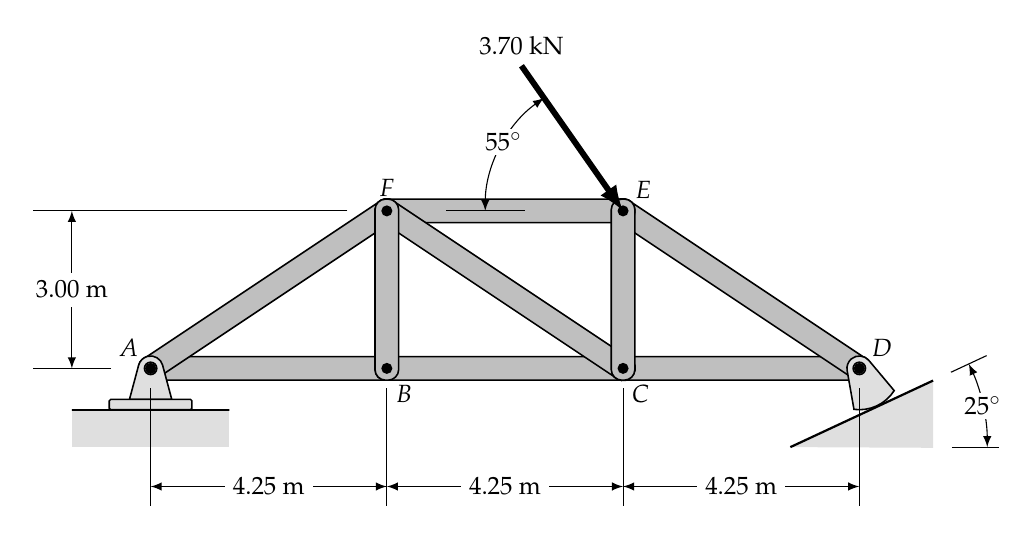
\begin{tikzpicture}[scale=\scale]
	\def\thickness{thick}
	% \def\stroke{black}
	\def\hi{.15}
	\def\radii{\hi}
	\def\extend{\hi}
	\small

	\coordinate (A) at (0, 0);
	\coordinate (B) at (3, 0);
	\coordinate (C) at (6, 0);
	\coordinate (D) at (9, 0);
	\coordinate (E) at (6, 2);
	\coordinate (F) at (3, 2);
	\coordinate (AA) at ($ (A)+(0,-0.5) $);

	% \gettikzxy{(AA)}{\aax}{\aay}	

	\Meme{A}{B}{gray!50}{gray!50}{black}{0.3}{0.135}{0.2}
	\Meme{B}{C}{gray!50}{gray!50}{black}{0.3}{0.135}{0.2}
	\Meme{C}{D}{gray!50}{gray!50}{black}{0.3}{0.135}{0.2}
	\Meme{E}{D}{gray!50}{gray!50}{black}{0.3}{0.135}{0.2}
	\Meme{E}{F}{gray!50}{gray!50}{black}{0.3}{0.135}{0.2}
	\Meme{A}{F}{gray!50}{gray!50}{black}{0.3}{0.135}{0.2}
	\Meme{C}{F}{gray!50}{gray!50}{black}{0.3}{0.135}{0.2}
	\Meme{B}{F}{gray!50}{gray!50}{black}{0.3}{0.135}{0.2}
	\Meme{C}{E}{gray!50}{gray!50}{black}{0.3}{0.135}{0.2}
	
	\fill[gray!25] ($ (A)-(1,0.525) $) rectangle ($ (A)+(1,-1) $);
	\draw[thick] ($ (A)-(1,0.525) $) rectangle ($ (A)+(1,-0.525) $);
	\fill[gray!25] ($ (D)+(-0.875,-1) $) -- ++(25:2) -- +(-90:0.854) -- cycle;
	\draw[thick] ($ (D)+(-0.875,-1) $) -- ++(25:2);

	\PC{A}{gray!25}{black}{0.525}{0.2}
	\Rocker[25]{D}{gray!25}{black}{0.525}{0.2}
	

	\draw ($ (A)+(0,-0.25) $) -- +(0,-1.5);
	\draw ($ (B)+(0,-0.25) $) -- +(0,-1.5);
	\draw ($ (C)+(0,-0.25) $) -- +(0,-1.5);
	\draw ($ (D)+(0,-0.25) $) -- +(0,-1.5);

	\draw[line width=0.75mm, latex-] (E) -- +(125:2.25) node[above] {$3.70$ kN};
	\draw ($ (E)+(-1.25,0) $)  -- ($ (E)+(-2.25,0) $);
	\draw[latex-latex] ($ (E)+(-1.75,0) $)  arc (180:125:1.75);
	\path  ($ (E)+(150:1.75) $) node[fill=white, inner sep=0.5mm] {\small $55^\circ$};

	\draw ($ (A)-(0.5, 0) $) -- ($ (A)-(1.5, 0) $);
	\draw ($ (F)-(0.5, 0) $) -- ($ (F)-(4.5, 0) $);
	\draw[ latex-latex] ($ (A)-(1, 0) $) -- node[fill=white]{$3.00\text{ m}$}($ (F)-(4, 0) $);

	\draw[ latex-latex] ([yshift=-1.5cm]A) -- node[fill=white]{$4.25\text{ m}$}([yshift=-1.5cm]B);
	\draw[ latex-latex] ([yshift=-1.5cm]B) -- node[fill=white]{$4.25\text{ m}$}([yshift=-1.5cm]C);
	\draw[ latex-latex] ([yshift=-1.5cm]C) -- node[fill=white]{$4.25\text{ m}$}([yshift=-1.5cm]D);

	 \draw ($ (D)+(-0.875,-1)+(25:2.25) $) -- +(25:0.5);
	\draw ($ (D)+(-0.875,-1)+(0:2.05) $) -- +(0:0.6);
	 \draw[latex-latex] ($ (D)+(-0.875,-1)+(0:2.5) $)  arc (0:25:2.5);
	 \path  ($ (D)+(-0.875,-1)+(12:2.5) $) node[fill=white, inner sep=0.5mm] {\small $25^\circ$};

	\fill[black] (A) circle (2pt) node[above left, outer sep=0.5mm] {$A$};
	\fill[black] (B) circle (2pt) node[below right, yshift=-1mm] {$B$};
	\fill[black] (C) circle (2pt) node[below right, yshift=-1mm] {$C$};
	\fill[black] (D) circle (2pt) node[above right, outer sep=0.5mm] {$D$};
	\fill[black] (E) circle (2pt) node[above right, outer sep=0.5mm] {$E$};
	\fill[black] (F) circle (2pt) node[above, outer sep=0.75mm] {$F$};

\end{tikzpicture}

  }
\end{textblock*}
\begin{textblock*}{\textwidth}(1in, 2.75in)
  \centering 
	\tikz{%color
  	\coordinate (A) at (0, 0);
    \coordinate (B) at (3, 0);
    \coordinate (C) at (6, 0);
    \coordinate (D) at (9, 0);
    \coordinate (E) at (6, 2);
    \coordinate (F) at (3, 2);

    \filldraw[draw=black, fill=gray!25] (A)--(F)--(E)--(D)--cycle;

    \draw ($ (A)+(0,-0.25) $) -- +(0,-1.5);
    \draw ($ (C)+(0,-0.25) $) -- +(0,-1.5);
    \draw ($ (D)+(0,-0.25) $) -- +(0,-1.5);
    \draw[ latex-latex] ([yshift=-1.5cm]A) -- node[fill=white]{$8.50\mathsf{ m}$}([yshift=-1.5cm]C);
	  \draw[ latex-latex] ([yshift=-1.5cm]C) -- node[fill=white]{$4.25\mathsf{ m}$}([yshift=-1.5cm]D);

    \fill[black] (A) circle (2pt) node[above left, outer sep=0.5mm] {$A$};
    \fill[black] (D) circle (2pt) node[above right, outer sep=0.5mm] {$D$};
    \fill[black] (E) circle (2pt) node[above right, outer sep=0.5mm] {$E$};

    \draw ($ (A)-(0.5, 0) $) -- ($ (A)-(1.5, 0) $);
    \draw ($ (F)-(0.5, 0) $) -- ($ (F)-(4.5, 0) $);
    \draw[ latex-latex] ($ (A)-(1, 0) $) -- node[fill=white]{$3.00\mathsf{ m}$}($ (F)-(4, 0) $);

    \draw[ultra thick, -latex] (A)--+(0,1.5) node[right] {$ R_{Ay} $};
    \draw[ultra thick, -latex] (A)--+(1.5,0) node[above] {$ R_{Ax} $};

    \draw[ultra thick, -latex] (D)--+(115:2) node[above] {$ R_D $};
    \draw[latex-latex] ($ (D)+(115:1.5) $) arc (115:180:1.5) node[midway, fill=white] {$ 65\deg $} ; 

    \draw[ultra thick, latex-] (E) -- +(125:2.25) node[left] {$3.70$ kN};
	  % \draw ($ (E)+(-1.25,0) $)  -- ($ (E)+(-2.25,0) $);
	  \draw[latex-latex] ($ (E)+(-1.5,0) $)  arc (180:125:1.5) node[midway, fill=white, inner sep=0.5mm] {\small $55^\circ$};
  }
  \begin{align*}
    \Sigma M_A &= (R_D\sin 65\deg)\cd(12.75\,\mathsf{m})-(3.70\,\mathsf{kN}\cd \sin 55\deg)\cd(8.50\,\mathsf{m})-(3.70\,\mathsf{kN}\cd \cos 55\deg)\cd(3.00\,\mathsf{m}) \\[0.25em]
    &= R_D\cd 11.555\,\mathsf{m} - 32.129\,\mathsf{kN\cd m} = 0 \\[0.25em]
    \Ra R_D &= \frac{32.129\,\mathsf{kN\cd m}}{11.555\,\mathsf{m}} = 2.7805\,\mathsf{kN}
  \end{align*}
 
  \large\pars
  \cmini{
    \centering
  The reaction at $D$ is \underline{$\bm{2.78\,}${\bf kN}} at \underline{$\bm{115\deg}$} measured counter-clockwise from the positive $x$-axis.
  }
  \normalsize

\end{textblock*}
\begin{textblock*}{0.7\textwidth}(1in, 6.875in)

  \begin{align*}
    \Sigma F_x &= R_{Ax}+(3.70\,\mathsf{kN})\cd\cos 55\deg-R_D\cos 65\deg = 0 \\[0.25em]
    \Ra R_{Ax} &= 2.7805\,\mathsf{kN}\cd\cos 65\deg-(3.70\,\mathsf{kN})\cd\cos 55\deg \\[0.25em]
    &= -0.94714\,\mathsf{kN} \\\\
    \Sigma F_y &= R_{Ay}+R_D\sin 65\deg-  (3.70\,\mathsf{kN})\cd\sin 55\deg = 0 \\[0.25em]
    \Ra R_{Ay} &= (3.70\,\mathsf{kN})\cd\sin 55\deg -2.7805\,\mathsf{kN}\cd\sin 65\deg\\[0.25em]
    &= 0.51087\,\mathsf{kN} \\\\
    R_A &= \sqrt{(-0.94714\,\mathsf{kN})^2+(-0.51087\,\mathsf{kN})^2} = 1.0761\,\mathsf{kN} \\[0.25em]
    \theta & = \tan^{-1}\left[\frac{0.51087}{0.94714}\right] = 28.342\deg       \\
  \end{align*}

  
\end{textblock*}

\begin{textblock*}{0.25\textwidth}(6in, 8.325in)
   \tikz{
				\draw[-latex, thick] (0,0) -- +(0,2)node[above]{$0.51087\,\text{kN}$};
				\draw[-latex, thick] (0,0) -- node[fill=white, below, outer sep=0.65mm]{$0.94714\,\text{kN}$}+(-4,0);
				\draw[-latex, thick, gray] (0,0) -- +(-4,2);
				\node at (-0.875,0.225) {$\theta$};
			}
\end{textblock*}

\begin{textblock*}{0.8\textwidth}(0.3\textwidth, 10.125in)
  \large\centering
  The reaction at $A$ is \underline{$\bm{1.08\,}${\bf kN}} at \underline{$\bm{152\deg}$} measured counter-clockwise from the positive $x$-axis.
\end{textblock*}

%%%%%%%%%%%%%%%%%%%%%%%%%%%%%%%%%%%%%%%%%%%%%%%%%%%%%%%%%%%%%%%%%%%%%%%%%%%%%%%%%%%%%%%%%%%%%%%%%%%%
% page 4
%%%%%%%%%%%%%%%%%%%%%%%%%%%%%%%%%%%%%%%%%%%%%%%%%%%%%%%%%%%%%%%%%%%%%%%%%%%%%%%%%%%%%%%%%%%%%%%%%%%%

~\newpage
\begin{textblock*}{3in}(1in, 0.1in)
	\cbox{
		\underbar{\bf Exercise 2:} Determine the reactions at the pinned connection and the tension in the cable.
	}
\end{textblock*}
\begin{textblock*}{3.25in}(4.525in, 0.1in)
	\cbox{
    \centering
    \def\scale{0.5}
    
	\tikz[scale=\scale]{
		\small
		\coordinate (A) at (0,0);
		\coordinate (B) at (4,0);
		\coordinate (C) at (7,0);
		\coordinate (D) at (8,0);
		\coordinate (E) at (8,6);
		\coordinate (F) at (9,0);

		\draw (A) circle (2pt);
		\draw (B) circle (2pt);
		\draw (C) circle (2pt);
		\draw (D) circle (2pt);
		\draw (E) circle (2pt);

		\fill[fill=white] (-2,-4) rectangle (10,8.5);
		\def\hi{0.375}
		\def\twohi{2*\hi}
		\def\threehi{3*\hi}
		\def\innerr{\hi}
		\def\outerr{3*\hi}
		\def\inneroffset{2*\hi}
		\def\outeroffset{\hi}


		\Meme{A}{F}{Gray!50}{Gray!50}{black}{1}{0.25}{0.25}
		% \pgfoonew \beam =new beam(A, F,Tan3,Gray!50, 0.5, 0.5, 0.5)
		\fill[gray!50] ($ (A)+(-1,-2) $) rectangle ($ (A)+(-2,2) $);
		\draw[thick, gray!50] ($ (A)+(-1,-2) $) -- ($ (A)+(-1,2) $);
		\PC[-90]{A}{gray!50}{black}{1}{0.25};

		\draw[line width=1mm] ($ (D)+(0.5, 0)$) -- ++(0,6)arc(0:150:0.5) -- (B);

		\fill[gray!50] ($ (E)+(-2,1) $) rectangle ($ (E)+(2,2) $);
		% \draw[thick, gray] ($ (E)+(-2,1) $) -- +(4,0);
		 \Pulley[180]{E}{gray!50}{black}{1}{0.25}

		\draw[-latex, line width=0.75 mm] (C) -- +(0, -3.5) node[left] {\large $2.20\text{ kN}$};

		\fill (A) circle (1.5mm);
		\fill (B) circle (1.5mm);
		\fill (C) circle (1.5mm);
		\fill ($(D)+(0.5,0)$) circle (1.5mm);
		\fill ($(E)$) circle (1.5mm);

		\draw ($ (D)+(0.5,-.75) $) -- +(0, -1.5);
		\draw ($ (B)+(0,-.75) $) -- +(0, -1.5);
		\draw ($ (A)+(0,-.75) $) -- +(0, -1.5);
		%
		\draw[latex-latex] ($ (A)+(0,-1.5) $) -- node[fill=white] {$4.00\;\text{m}$}($ (B)+(0,-1.5) $);
		\draw[latex-latex] ($ (B)+(0,-1.5) $) -- node[fill=white] {$3.00\;\text{m}$}($ (C)+(0,-1.5) $);
		\draw[latex-latex] ($ (C)+(0,-1.5) $) -- ($ (D)+(0.5,-1.5) $);

		\node[right, fill=white,outer sep= 1mm, inner sep=1mm] at ($ (C)+(0, -2) $) {$ 1.50\text{ m}$};

		\draw[latex-latex] ($ (B)+(2,0) $)arc(0:60:2);
		\draw ($ (B)+(1.5,0) $)-- +(1,0);
		\node[fill=white, inner sep=0.5mm] at ($ (B)+(30:2.125) $) {$60\deg$};
	}


  }
\end{textblock*}
\begin{textblock*}{3.5in}(1in, 1.25in)
  \centering 
	\tikz[scale=0.75]{%color
  	\coordinate (A) at (0,0);
		\coordinate (B) at (4,0);
		\coordinate (C) at (7,0);
		\coordinate (D) at (8,0);
		\coordinate (E) at (8,6);
		\coordinate (F) at (9,0);

    \draw[gray!40, line width=0.5cm, line cap = round] (A)--(D);
    \draw[ultra thick, -latex] (D)--+(0,2)node[above]{$ T $};
    \draw[ultra thick, -latex] (B)--+(60:2.5)node[above]{$ T $};
    \draw[ultra thick, -latex] (C)--+(270:2.5)node[below]{$ 2.20\,\mathsf{kN} $};
    \draw[ultra thick, -latex] (A)--+(0,2)node[right]{$ R_{Ay} $};
    \draw[ultra thick, -latex] (A)--+(2,0)node[above]{$ R_{Ax} $};

    \draw[latex-latex] ($ (B)+(1.5,0) $)arc(0:60:1.5)node[midway, fill=white]{$ 60\deg $};

    \draw[latex-latex] ($ (A)+(0,-1.5) $) -- node[fill=white] {$4.00\;\mathsf{m}$}($ (B)+(0,-1.5) $);
		\draw[latex-latex] ($ (B)+(0,-1.5) $) -- node[fill=white] {$3.00\;\mathsf{m}$}($ (C)+(0,-1.5) $);
		\draw[latex-latex] ($ (C)+(0,-1.5) $) -- node[fill=white,rotate=90] {$1.50\;\mathsf{m}$}($ (D)+(0,-1.5) $);

    \draw ($ (D)+(0,-.75) $) -- +(0, -1.5);
		\draw ($ (B)+(0,-.75) $) -- +(0, -1.5);
		\draw ($ (A)+(0,-.75) $) -- +(0, -1.5);
  }

  \begin{align*}
    \Sigma M_A &= (T\sin 60\deg)\cd(4.00\,\mathsf{m})+T\cd(8.50\,\mathsf{m})-(2.20\,\mathsf{kN})\cd(7.00\,\mathsf{m}) = 0 \\[0.25em]
    \Ra T &= \frac{(2.20\,\mathsf{kN})\cd(7.00\,\mathsf{m})}{(4.00\,\mathsf{m})\cd(\sin 60\deg)+(8.50\,\mathsf{m})} = 1.2872\,\mathsf{kN} \\\\
    \Sigma F_x &= R_{Ax}+T\cos 60\deg = 0 \\[0.25em]
    \Ra R_{Ax} &= -(1.2872\,\mathsf{kN})\cd\cos 60\deg = -0.64359\,\mathsf{kN} \\\\
    \Sigma F_y &= R_{Ay} +T\sin 60\deg +T - 2.20\,\mathsf{kN} = 0 \\[0.25em]
    \Ra R_{Ay} &= 2.20\,\mathsf{kN} -(1.2872\,\mathsf{kN})\cd(1+\sin 60\deg) = -0.20195\,\mathsf{kN} \\\\
    R_A &= \sqrt{(-0.64359\,\mathsf{kN})^2+(-0.20195\,\mathsf{kN})^2} = 0.67453\,\mathsf{kN}\\[0.25em]
    \theta &= \tan^{-1}\left[\frac{-0.20195}{-0.64359}\right] = 17.421\deg
  \end{align*}
  \large\centering\parb
  The tension in the cable is \underline{$\bm{1.29}\,\mathsf{\bf kN}$} \parb
  The reaction at $A$ is \underline{$\bm{0.675\,}${\bf kN}} at \underline{$\bm{197\deg}$} measured counter-clockwise from the positive $x$-axis.

\end{textblock*}
\begin{textblock*}{0.25\textwidth}(5.75in, 5.5in)
   \tikz{
				\draw[-latex, thick] (0,0) -- +(0,-2)node[below]{$0.20195\,\mathsf{kN}$};
				\draw[-latex, thick] (0,0) -- +(-4,0)node[fill=white, above, outer sep=0.65mm]{$0.64359\,\mathsf{kN}$};
				\draw[-latex, thick, gray] (0,0) -- +(-4,-2);
				\node at (-0.875,-0.225) {$\theta$};
			}
\end{textblock*}



%%%%%%%%%%%%%%%%%%%%%%%%%%%%%%%%%%%%%%%%%%%%%%%%%%%%%%%%%%%%%%%%%%%%%%%%%%%%%%%%%%%%%%%%%%%%%%%%%%%%
% page 5
%%%%%%%%%%%%%%%%%%%%%%%%%%%%%%%%%%%%%%%%%%%%%%%%%%%%%%%%%%%%%%%%%%%%%%%%%%%%%%%%%%%%%%%%%%%%%%%%%%%%

~\newpage
\begin{textblock*}{3in}(1in, 0.1in)
	\cbox{
		\underbar{\bf Example 3:} The roller and the pinned connection are on slopes
    inclined at $21\deg$ to the horizontal; they are both at the same elevation. \parm Determine the reactions at the pinned connection and the tension in the cable.
	}
\end{textblock*}
\begin{textblock*}{3.25in}(4.525in, 0.1in)
	\cbox{
    \centering
    \def\scale{1}
    % !TEX root = ../../Beamer/06EquilibriumOfRigidBodies/06ERB.tex

\tikz[scale=\scale]{
	\coordinate (O) at (0,0);
	\coordinate (OO) at (0,0.175);
	\coordinate (A) at ($(O)+(35:3)$);
	\coordinate (B) at ($(O)+(65:3)$);
	\coordinate (C) at ($(O)+(90:3)$);
	\coordinate (D) at ($(O)+(115:3)$);
	\coordinate (E) at ($(O)+(145:3)$);
	\coordinate (top) at ($(C)+(0,1)$);

  \gettikzxy{(A)}{\Ax}{\Ay};
  \gettikzxy{(B)}{\Bx}{\By};
  \gettikzxy{(C)}{\Cx}{\Cy};
  \gettikzxy{(D)}{\Dx}{\Dy};
  \gettikzxy{(E)}{\Ex}{\Ey};
  \gettikzxy{(top)}{\tx}{\ty};

	\filldraw[rounded corners=4pt, fill=Gray!50] (OO)-- ++(158:4)-- ++(0,-2)-- ++(7.4175,0)-- +(0,2) -- cycle;
	\filldraw[fill=Gray!50]($(A)+(35:0.25)$)arc(35:145:3.25)arc(145:325:0.25)arc(145:35:2.75)arc(215:395:0.25);
	\Roller[-22]{E}{myGray4}{black}{0.5}{0.125};
	\PC[22]{A}{myGray4}{black}{0.51}{0.125};
  \footnotesize
  \draw[very thick,  -Latex] (B)-- +(0,-1.2)node[below, black]{\scriptsize $8.00\,$kN};
  \draw[very thick,  -Latex] (C)-- +(0,-1.475)node[below, black]{\scriptsize $10.0\,$kN};
  \draw[very thick,  -Latex] (D)-- +(0,-1.2)node[below, black]{\scriptsize $12.0\,$kN};
  \draw[very thick,  -Latex] (D)-- +(-1, 0)node[yshift=0.25cm,xshift=0.375cm, black]{\scriptsize$5.00\,$kN};

  \filldraw[ball color=DarkOliveGreen4, thin] (B) circle (0.875mm);
  \filldraw[ball color=DarkOliveGreen4, thin] (C) circle (0.875mm);
  \filldraw[ball color=DarkOliveGreen4, thin] (D) circle (0.875mm);

  \draw[thin, gray] ($(A)+(0,0.7)$) -- (\Ax,\ty);
  \draw[thin, gray] ($(B)+(0,0.5)$) -- (\Bx,\ty);
  \draw[thin, gray] ($(C)+(0,0.45)$) -- (\Cx,\ty);
  \draw[thin, gray] ($(D)+(0,0.5)$) -- (\Dx,\ty);
  \draw[thin, gray] ($(E)+(0,0.6)$) -- (\Ex,\ty);
  \draw[thin, gray] ($(D)+(-1.125,0)$) -- (\Ex-0.75cm,\Dy);
  \draw[thin, gray] ($(E)+(-.375,0)$) -- (\Ex-0.75cm,\Ey);


  \def\dimy{\ty-0.25cm}
  \draw[latex-latex] (\Ex,\dimy)--node[fill=white,inner sep=0.15mm]{\scriptsize $2.50\,$m}(\Dx,\dimy);
  \draw[latex-latex] (\Dx,\dimy)--node[fill=white,inner sep=0.15mm]{\scriptsize $2.50\,$m}(\Cx,\dimy);
  \draw[latex-latex] (\Cx,\dimy)--node[fill=white,inner sep=0.15mm]{\scriptsize $2.50\,$m}(\Bx,\dimy);
  \draw[latex-latex] (\Bx,\dimy)--node[fill=white,inner sep=0.15mm]{\scriptsize $2.50\,$m}(\Ax,\dimy);
  \draw[latex-latex] (\Ex-0.5cm,\Dy)--node[fill=white,inner sep=0.15mm]{\scriptsize $2.10\,$m}(\Ex-0.5cm,\Ey);
}

  }
\end{textblock*}
\begin{textblock*}{4in}(1in, 1.75in)
  \centering
	\tikz[scale=1.25]{%color
    \coordinate (O) at (0,0);
	\coordinate (OO) at (0,0.175);
	\coordinate (A) at ($(O)+(35:3)$);
	\coordinate (B) at ($(O)+(65:3)$);
	\coordinate (C) at ($(O)+(90:3)$);
	\coordinate (D) at ($(O)+(115:3)$);
	\coordinate (E) at ($(O)+(145:3)$);
	\coordinate (top) at ($(C)+(0,1)$);

  \gettikzxy{(A)}{\Ax}{\Ay};
  \gettikzxy{(B)}{\Bx}{\By};
  \gettikzxy{(C)}{\Cx}{\Cy};
  \gettikzxy{(D)}{\Dx}{\Dy};
  \gettikzxy{(E)}{\Ex}{\Ey};
  \gettikzxy{(top)}{\tx}{\ty};

  \fill[fill=Gray!50]($(A)+(35:0.25)$)arc(35:145:3.25)arc(145:325:0.25)arc(145:35:2.75)arc(215:395:0.25);

  \draw[very thick, -latex] (A)--+(1,0)node[below]{$ R_{Ax} $};
  \draw[very thick, -latex] (A)--+(0,1)node[right]{$ R_{Ay} $};
  \draw[very thick, -latex] (E)--+(69:0.875)node[right]{$ R_{B} $};
  \draw[very thick, -latex] (B)--+(-90:1)node[below]{$ 8.00\,\mathsf{kN} $};
  \draw[very thick, -latex] (C)--+(-90:0.75)node[below]{$ 10.0\,\mathsf{kN} $};
  \draw[very thick, -latex] (D)--+(-90:1)node[below]{$ 12.0\,\mathsf{kN} $};
  \draw[very thick, -latex] (D)--+(180:1)node[above]{$ 5.00\,\mathsf{kN} $};

  \node[xshift=0.25cm, yshift=-0.25cm] at (A){$ A $};
  \node[xshift=-0.325cm, yshift=-0.25cm] at (E){$ B $};

   \draw[thin, gray] ($(A)+(0,0.7)$) -- (\Ax,\ty);
  \draw[thin, gray] ($(B)+(0,0.5)$) -- (\Bx,\ty);
  \draw[thin, gray] ($(C)+(0,0.45)$) -- (\Cx,\ty);
  \draw[thin, gray] ($(D)+(0,0.5)$) -- (\Dx,\ty);
  \draw[thin, gray] ($(E)+(0,0.6)$) -- (\Ex,\ty);
  \draw[thin, gray] ($(D)+(-1.125,0)$) -- (\Ex-0.75cm,\Dy);
  \draw[thin, gray] ($(E)+(-.375,0)$) -- (\Ex-0.75cm,\Ey);

  \draw[latex-latex] ($(E)+(0.625,0)$) arc(0:69:0.625) node[midway, inner sep=0, fill=white]{$ 69\deg $};

   \def\dimy{\ty-0.25cm}
  \draw[latex-latex] (\Ex,\dimy)--node[fill=white,inner sep=0.15mm]{\footnotesize $2.50\,$m}(\Dx,\dimy);
  \draw[latex-latex] (\Dx,\dimy)--node[fill=white,inner sep=0.15mm]{\footnotesize $2.50\,$m}(\Cx,\dimy);
  \draw[latex-latex] (\Cx,\dimy)--node[fill=white,inner sep=0.15mm]{\footnotesize $2.50\,$m}(\Bx,\dimy);
  \draw[latex-latex] (\Bx,\dimy)--node[fill=white,inner sep=0.15mm]{\footnotesize $2.50\,$m}(\Ax,\dimy);
  \draw[latex-latex] (\Ex-0.5cm,\Dy)--node[fill=white,inner sep=0.15mm]{\footnotesize $2.10\,$m}(\Ex-0.5cm,\Ey);
  }
\end{textblock*}
\begin{textblock*}{4.75in}(1in, 3.25in) 
  \begin{align*}
    \Sigma M_A &= (8.00\,\mathsf{kN})\cd(2.50\,\mathsf{m})+(10.0\,\mathsf{kN})\cd(5.00\,\mathsf{m})+(12.0\,\mathsf{kN})\cd(7.50\,\mathsf{m})\\
    &\qquad\qquad +(5.00\,\mathsf{kN})\cd(2.10\,\mathsf{m})-(R_B\sin 69\deg)\cd(10.0\,\mathsf{m})\\[0.25em]
    &= 170.5\,\mathsf{kN\cd m}-(9.3358\,\mathsf{m})\cd R_B = 0 \\[0.25em]
    \Ra R_B &= \frac{170.5\,\mathsf{kN\cd m}}{9.3358\,\mathsf{m}} = 18.263\,\mathsf{kN} \\\\\\
    \Sigma F_x &= R_B\cd\cos 69\deg + R_{Ax} - 5.00\,\mathsf{kN} = 0 \\[0.25em]
    \Ra R_{Ax} &= 5.00\,\mathsf{kN} - (18.623\,\mathsf{kN})\cd\cos 69\deg = -1.6739\,\mathsf{kN}\\\\\\
    \Sigma F_y &= R_{Ay}+R_B\sin 69\deg -(12.0\,\mathsf{kN}+10.0\,\mathsf{kN}+8.00\,\mathsf{kN}) = 0 \\[0.25em]
    R_{Ay} &= 30.0\,\mathsf{kN}-(18.263\,\mathsf{kN})\cd\sin 69\deg = 12.950\,\mathsf{kN} \\\\\\
    R_A &= \sqrt{(-1.6739\,\mathsf{kN})^2+(12.950\,\mathsf{kN})^2} = 13.058\,\mathsf{kN}\\[0.25em]
    \theta &= \tan^{-1}\left[\frac{12.950}{1.6739}\right] = 82.635\deg
  \end{align*}
  \large\parb\centering
  The reaction at the roller is  \underline{$\bm{18.3}\,\mathsf{\bf kN}$} at \underline{$\bm{69\deg}$} measured counter-clockwise from the positive $x$-axis.
  \parb
  The reaction at the pinned connection is \underline{$\bm{13.1\,}${\bf kN}} at \underline{$\bm{97.4\deg}$} measured counter-clockwise from the positive $x$-axis.
\end{textblock*}
\begin{textblock*}{2in}(7in, 5in) 
  \tikz{%color
    \draw[very thick, -latex] (0,0)--(-1,0)node[below]{$1.6739$};
    \draw[very thick, -latex] (0,0)--(0,6)node[above]{$12.950$};
    \draw[ultra thick, -latex, gray] (0,0)--(-1,6)node[left]{$R_A$};
    \node at (-0.25,0.25) {$ \theta $};
  }
\end{textblock*}

%%%%%%%%%%%%%%%%%%%%%%%%%%%%%%%%%%%%%%%%%%%%%%%%%%%%%%%%%%%%%%%%%%%%%%%%%%%%%%%%%%%%%%%%%%%%%%%%%%%%
% page 6
%%%%%%%%%%%%%%%%%%%%%%%%%%%%%%%%%%%%%%%%%%%%%%%%%%%%%%%%%%%%%%%%%%%%%%%%%%%%%%%%%%%%%%%%%%%%%%%%%%%%

~\newpage
\begin{textblock*}{2.5in}(1in, 0.1in)
	\cbox{
		\underbar{\bf Example 4:} \parm The roller at $B$ is in a smooth slot. \parm Determine the reactions at $A$ and $B$.
	}
\end{textblock*}
\begin{textblock*}{3.75in}(4.025in, 0.1in)
	\cbox{
    \centering
    \def\scale{0.575}
    
\tikz[scale=\scale]{
	\small
	\coordinate (A) at (0,0);
	\coordinate (B) at (8,0);
	\coordinate (C) at (8,4);
	\coordinate (D) at (11,4);
	\coordinate (E) at (5,0);
	\coordinate (F) at (8,2);

	\draw (B) circle (2pt);
	\draw (C) circle (2pt);

	\fill[fill=white] (-3,-2.5) rectangle (13,5.25);
	\def\hi{0.375}
	\def\twohi{2*\hi}
	\def\threehi{3*\hi}
	\def\innerr{\hi}
	% \def\outerr{3*\hi}
	\def\inneroffset{2*\hi}
	\def\outeroffset{\hi}

	\Ronly{D}{gray}{black}{0.6}{0.25}

	\draw[fill=gray!50, draw=black, thick] ($ (A)+(0,\hi) $) -- ($ (B)+(-\twohi,\hi) $) arc(-90:0:\hi) -- ($ (C)+(-\hi,-\twohi) $) arc(180:90:\threehi) -- ($ (D)+(0,\hi) $) arc(90:-90:\hi) -- ($ (C)+(\twohi,-\hi) $)arc(90:180:\hi) -- ($ (B)+(\hi,\twohi) $)arc(0:-90:\threehi) -- ($ (A)+(0,-\hi) $)arc (270:90:\hi);
	\shadedraw[ball color=gray, black, thick] (D) circle (2mm);
	\PC{A}{gray}{black}{1}{0.25}

	\fill[gray] ($ (A)+(-2,-1) $) rectangle ($ (A)+(2,-1.65) $);
	\fill[gray] ($ (D)+(-1.5,-.6) $) rectangle ($ (D)+(2,-1.25) $);
	\fill[gray] ($ (D)+(-1.5,.6) $) rectangle ($ (D)+(2,1.25) $);
	\draw[thick, gray!50!black] ($ (A)+(-2,-1) $) -- ($ (A)+(2,-1) $);
	\draw[thick, gray!50!black] ($ (D)+(-1.5,.6) $) -- ($ (D)+(2,0.6) $);
	\draw[thick, gray!50!black] ($ (D)+(-1.5,-.6) $) -- ($ (D)+(2,-0.6) $);

	\draw ($ (D)+(0,-1) $) -- +(0, -5.5);
	\draw ($ (B)+(0,-0.5) $) -- +(0, -2);
	\draw ($ (E)+(0,-0.5) $) -- +(0, -2);
	\draw ($ (A)+(0,-0.5) $) -- +(0, -2);
	\draw ($ (D)+(-2,0) $) -- +(-3.25, 0);
	\draw ($ (B)+(-0.5,0) $) -- +(-2, 0);
	\draw ($ (E)+(-2.75,0) $) -- ($ (E)+(-1.75,0) $);
	\draw[latex-latex] ($ (E)+(125:2.25) $)arc(125:180:2.25);
	\node at ($ (E)+(153:2.25) $) [fill=white]{$55^\circ$};

	\draw[latex-latex] ($ (A)+(0,-2) $) -- node[fill=white] {$2.50\;\mathsf{m}$}($ (E)+(0,-2) $);
	\draw[latex-latex] ($ (E)+(0,-2) $) -- node[fill=white] {$1.50\;\mathsf{m}$}($ (B)+(0,-2) $);
	\draw[latex-latex] ($ (B)+(0,-2) $) -- node[fill=white] {$1.50\;\mathsf{m}$}($ (D)+(0,-6) $);
	\draw[latex-latex] ($ (C)+(-1.75,0) $) -- node[fill=white] {$2.00\;\mathsf{m}$}($ (B)+(-1.75,0) $);

	\draw[latex-, ultra thick] (E) -- +(125:2.75) node[above,black] {$1.24\;\mathsf{kN}$};
	\Couple{F}{black}{0.75}{.75}
  % \draw[-Straight Barb, ultra thick, statsMaroon] ($ (F)+(-70:0.875) $)arc(-70:289:0.875) node[below right, fill=white, inner sep=1mm, outer sep=1mm] {$\bm{ 3.75}\;\text{\bfseries{kN}}\bm\cdot\text{\bfseries m}$};
	\node[xshift=1cm, yshift=-0.5cm] at (F) {$1.75\,\mathsf{kN\cd m} $};

	\node[above left, outer sep = 1mm] at (A) {\large $A$};
	\node[right, outer sep = 3mm] at (D) {\large $B$};

}

  }
\end{textblock*}
\begin{textblock*}{2.5in}(1in, 1.325in)
	\centering
  \tikz[scale=0.5]{%color

    \def\hi{0.375}
    \def\twohi{2*\hi}
    \def\threehi{3*\hi}
    \def\innerr{\hi}
    % \def\outerr{3*\hi}
    \def\inneroffset{2*\hi}
    \def\outeroffset{\hi}

    \coordinate (A) at (0,0);
    \coordinate (B) at (8,0);
    \coordinate (C) at (8,4);
    \coordinate (D) at (11,4);
    \coordinate (E) at (5,0);
    \coordinate (F) at (8,2);

    \fill[gray!50] ($ (A)+(0,\hi) $) -- ($ (B)+(-\twohi,\hi) $) arc(-90:0:\hi) -- ($ (C)+(-\hi,-\twohi) $) arc(180:90:\threehi) -- ($ (D)+(0,\hi) $) arc(90:-90:\hi) -- ($ (C)+(\twohi,-\hi) $)arc(90:180:\hi) -- ($ (B)+(\hi,\twohi) $)arc(0:-90:\threehi) -- ($ (A)+(0,-\hi) $)arc (270:90:\hi);

    \fill (A) circle (2pt) node[left,xshift=-0.125cm] {$ A $};
	  \fill (D) circle (2pt)node[right,xshift=0.125cm] {$ B $};

    \draw[latex-latex] ($ (A)+(0,-2) $) -- node[fill=white,inner sep=0.5mm] {$2.50\;\mathsf{m}$}($ (E)+(0,-2) $);
    \draw[latex-latex] ($ (E)+(0,-2) $) -- node[fill=white,inner sep=0.5mm] {$1.50\;\mathsf{m}$}($ (B)+(0,-2) $);
    \draw[latex-latex] ($ (B)+(0,-2) $) -- node[fill=white,inner sep=0.5mm] {$1.50\;\mathsf{m}$}($ (D)+(0,-6) $);
    \draw[latex-latex] ($ (C)+(-1.75,0) $) -- node[fill=white,inner sep=0.75mm] {$2.00\;\mathsf{m}$}($ (B)+(-1.75,0) $);

    \draw[latex-, thick] (E) -- +(125:2.75) node[above,black] {$1.24\;\mathsf{kN}$};
    \Couple{F}{black}{0.75}{.5}
    \node[xshift=1.2cm, yshift=-0.5cm, fill=white, inner sep = 0.5mm] at (F) {$1.75\,\mathsf{kN\cd m} $};

    \draw ($ (D)+(0,-1) $) -- +(0, -5.5);
    \draw ($ (B)+(0,-0.5) $) -- +(0, -2);
    \draw ($ (E)+(0,-0.5) $) -- +(0, -2);
    \draw ($ (A)+(0,-0.5) $) -- +(0, -2);
    \draw ($ (D)+(-2,0) $) -- +(-3.25, 0);
    \draw ($ (B)+(-0.5,0) $) -- +(-2, 0);
    \draw ($ (E)+(-2.75,0) $) -- ($ (E)+(-1.75,0) $);
    \draw[latex-latex] ($ (E)+(125:2.25) $)arc(125:180:2.25);
    \node at ($ (E)+(153:2.25) $) [fill=white]{$55^\circ$};

    \draw[thick, -latex] (A)--+(1.5,0)node[below]{$ R_{Ax}$};
    \draw[thick, -latex] (A)--+(0,1.5)node[left]{$ R_{Ay}$};
    \draw[thick, -latex] (D)--+(0,1.5)node[left]{$ R_B$};
  }
\end{textblock*}
\begin{textblock*}{4.75in}(1in,3.25in)
  

  \begin{align*}
    \Sigma M_A &= R_B\cd (5.50\,\mathsf{m})+1.75\,\mathsf{kN\cd m}-(1.24\,\mathsf{kN})\cd (2.50\,\mathsf{m}) = 0 \\[0.25em]
    \Ra R_B &= \frac{3.1\,\mathsf{kN\cd m}-1.75\,\mathsf{kN\cd m}}{5.50\,\textsf{m}} = 0.24545\,\textsf{kN}
  \end{align*}
  \cmini{
  \underline{\bf Note}: We began by assuming a reaction $R_B$ in the positive direction (that is, that the roller at $B$ was pressing down on the slot). Our result for $R_B$ is positive, so that initial assumption is correct. If $R_B$ had evaluated to a negative value, then the roller would be pressing upward on the slot and the reaction would be downward.
  }
  \begin{align*}
    \Sigma F_x &= R_{Ax}+(1.24\,\textsf{kN})\cd\cos 55\deg=0\\[0.25em]
    \Ra R_{Ax} &= -0.71123\,\textsf{kN} \\\\
    \Sigma F_y &= R_{Ay}+R_B -(1.24\,\textsf{kN})\cd\sin 55\deg=0\\[0.25em]
    \Ra R_{Ay} &= (1.24\,\textsf{kN})\cd\sin 55\deg-0.24545\,\textsf{kN} = 0.77030\,\textsf{kN} \\\\
    R_A &= \sqrt{(-0.71123\,\textsf{kN})^2+(0.77030\,\textsf{kN})^2} = 1.0484\,\textsf{kN}\\[0.25em]
    \theta &= \tan^{-1}\left[\frac{0.77030}{0.71123}\right] = 47.283\deg
  \end{align*}

  \large\parb\centering 
  The reaction at $A$ is \underline{$\bm{1.05\,\mathbf{\mathsf{kN}}}$} at \underline{$\bm{133\deg}$}, measured counter-clockwise from the positive $x$-axis. 
  \parb
  The reaction at $B$ is \underline{$\bm{0.245\,\mathbf{\mathsf{kN}}}$} at \underline{$\bm{90\deg}$}, measured counter-clockwise from the positive $x$-axis.
\end{textblock*}

\begin{textblock*}{2in}(6in, 5.25in) 
  \tikz{%color
    \draw[very thick, -latex] (0,0)--(-1.75,0)node[below]{$0.71123$};
    \draw[very thick, -latex] (0,0)--(0,1.875)node[above]{$0.77030$};
    \draw[ultra thick, -latex, gray] (0,0)--(-1.75,1.875)node[left]{$R_A$};
    \node at (-0.5,0.25) {$ \theta $};
  }
\end{textblock*}

%%%%%%%%%%%%%%%%%%%%%%%%%%%%%%%%%%%%%%%%%%%%%%%%%%%%%%%%%%%%%%%%%%%%%%%%%%%%%%%%%%%%%%%%%%%%%%%%%%%%
% page 7
%%%%%%%%%%%%%%%%%%%%%%%%%%%%%%%%%%%%%%%%%%%%%%%%%%%%%%%%%%%%%%%%%%%%%%%%%%%%%%%%%%%%%%%%%%%%%%%%%%%%

~\newpage
\begin{textblock*}{3in}(1in, 0.1in)
	\cbox{
		\underbar{\bf Example 5:} \parm $55-\textsf{kg}$ bar $AB$ has its centre of gravity at $G$. It is supported by a pinned connection at $A$ and a smooth peg at $C$. A cable is attached at $B$ and has a tensile force of $1.70\,\textsf{kN}$. The direction of the cable varies between $\theta = 60\deg$ and $\theta = 135\deg$.\parb
    What is the maximum reaction at $P$? Determine the reaction at $A$ for this reaction at $P$.
	}
\end{textblock*}
\begin{textblock*}{3.25in}(4.525in, 0.1in)
	\cbox{
    \centering
    \def\scale{0.875}
    % !TEX root = ../../Beamer/06EquilibriumOfRigidBodies/06ERBforDT.tex



\begin{tikzpicture}[scale=\scale]

	\coordinate (O) at (0, 0);
	\coordinate (B) at ($(O)+(36:6)$);
	\coordinate (G) at ($(O)!0.45!(B)$);
	\coordinate (P) at ($(O)+(36:4.15)$);

	\coordinate (D) at ($(G)!0.25!(B)$);
	\coordinate (E) at ($(G)!0.75!(B)$);
	\coordinate (C) at ($(D)!0.4!(E)$);

	\small

	\fill[top color = gray!50, bottom color=gray!50] ($(A)+(-1,-0.5)$) rectangle +(2,-0.5);
	\Meme{A}{B}{gray!25}{gray!25}{black}{0.5}{0.2}{.2}
	\Meme{D}{E}{white}{white}{black}{0.25}{0.1}{.2}
	\PC{A}{gray!50}{black}{0.5}{0.2}

	\node[yshift=1.25mm, xshift=-4mm , inner sep=2mm] at (A) {$A$};
	\filldraw (G) circle (1.5pt) node[yshift=-3mm, xshift=3mm , inner sep=2mm] {$G$};
	\filldraw (B) circle (1.5pt) node[yshift=3mm, xshift=3mm , inner sep=2mm] {$B$};
	\filldraw[ball color=LightCyan4] (P) circle (2.75pt) node[yshift=-3mm, xshift=3mm ] { $P$};
	\draw[-latex, very thick] (B) -- +(-38:3)node[below]{$1.70\,\textsf{kN}$};

	\draw ($(B)+(216:0.25)$) -- +(216:0.75);
	\draw[latex-latex] ($(B)+(-38:0.625)$)arc[start angle=322, end angle=217, radius=0.625]node[midway, fill=white, inner sep=0.35mm]{\large $\theta$};



	\draw ($(A)+(0:0.75)$) -- +(0:1.5);
	\draw ($(A)+(36:0.75)$) -- +(36:1.5);
	\draw[latex-latex] ($(A)+(-0:2)$)arc[start angle=0, end angle=36, radius=2]node[midway, fill=white, inner sep=.3mm]{\small $36\deg$};

	\draw ($(A)+(126:0.5)$) -- +(126:0.75);
	\draw ($(G)+(126:0.5)$) -- +(126:0.75);
	\draw ($(B)+(126:0.5)$) -- +(126:0.75);
	\draw ($(P)+(126:0.5)$) -- +(126:0.75);
	\footnotesize
	\draw[latex-latex]($(A)+(126:1)$) -- node[fill=white, inner sep=0.25mm, rotate=-30]{$550\,\textsf{mm}$}($(G)+(126:1)$);
	\draw[latex-latex]($(G)+(126:1)$) -- node[fill=white, inner sep=0.5mm, rotate=-30]{$300\,\textsf{mm}$}($(P)+(126:1)$);
	\draw[latex-latex]($(P)+(126:1)$) -- node[fill=white, inner sep=0.5mm, rotate=-30]{$350\,\textsf{mm}$}($(B)+(126:1)$);

\end{tikzpicture}

  }
\end{textblock*}

\begin{textblock*}{3in}(1in, 2.25in)
  
	\tikz{%color
    \coordinate (A) at (0, 0);
    \coordinate (B) at ($(O)+(36:6)$);
    \coordinate (G) at ($(O)!0.45!(B)$);
    \coordinate (P) at ($(O)+(36:4.15)$);

    \draw[line width = 0.5cm, line cap = round, gray!35] (A)--(B);
    \draw[very thick, -latex] (G)--+(0,-2) node[below] {$ 0.53955\,\textsf{kN} $};
    \draw[latex-latex] ($(G)+(0,-1.5)$) arc (-90:-144:1.5) node[fill=white, midway, inner sep=0.2mm] {\small $ 54.0\deg $};
    \draw[very thick, -latex] (A)--+(1,0)node[below]{$ R_{Ax}$};
    \draw[very thick, -latex] (A)--+(0,1)node[right]{$ R_{Ay}$};
    \draw[very thick, -latex] (P)--+(126:2)node[above]{$ R_P$};
    \draw[-latex, very thick] (B) -- +(-38:2)node[below]{$1.70\,\textsf{kN}$};
    \draw[latex-latex] ($(B)+(-38:0.625)$)arc[start angle=322, end angle=217, radius=0.625]node[midway, fill=white, inner sep=0.35mm]{\large $\theta$};

    \draw ($(A)+(126:0.5)$) -- +(126:0.75);
    \draw ($(G)+(126:0.5)$) -- +(126:0.75);
    \draw ($(B)+(126:0.5)$) -- +(126:0.75);
    \draw[latex-latex]($(A)+(126:1)$) -- node[fill=white, inner sep=0.25mm, rotate=-30]{$550\,\textsf{mm}$}($(G)+(126:1)$);
	\draw[latex-latex]($(G)+(126:1)$) -- node[fill=white, inner sep=0.5mm, rotate=-30]{$300\,\textsf{mm}$}($(P)+(126:1)$);
	\draw[latex-latex]($(P)+(126:1)$) -- node[fill=white, inner sep=0.5mm, rotate=-30]{$350\,\textsf{mm}$}($(B)+(126:1)$);

  \filldraw (A) circle (1.5pt) node [yshift=1.25mm, xshift=-4mm , inner sep=2mm] {$A$};
	\filldraw (G) circle (1.5pt) node[yshift=-3mm, xshift=3mm , inner sep=2mm] {$G$};
	\filldraw (B) circle (1.5pt) node[yshift=3mm, xshift=3mm , inner sep=2mm] {$B$};
	\filldraw (P) circle (1.5pt) node[yshift=-3mm, xshift=3mm ] { $P$};

  \draw [thin] (A)--(B);
  }
\end{textblock*}
\begin{textblock*}{5in}(2.875in,3.5in)
  \begin{align*}
    \Sigma M_A &= R_P\cd (850\,\textsf{mm})-(1.70\,\textsf{kN}\cd\sin \theta)(1200\,\textsf{mm})-(0.53955\,\textsf{kN}\cd\sin 54\deg)\cd (550\,\textsf{mm}) \\[0.25em]
    &= R_P\cd (0.850\,\textsf{m})-(2.0400\,\mathsf{kN\cd m})\cd\sin \theta - 0.23828\,\mathsf{kN\cd m} = 0 \\[0.25em]
    \Ra R_P &= \frac{(2.0400\,\mathsf{kN\cd m})\cd\sin \theta +0.23828\,\mathsf{kN\cd m}}{0.850\,\textsf{m}} = 2.4000\,\textsf{kN}\cd \sin\theta + 0.28033\,\textsf{kN} \\[0.25em]
    \Ra R_{P_{max}} &= 2.4000\,\textsf{kN}\cd \sin 90\deg + 0.28033\,\textsf{kN} = 2.6803\,\textsf{kN} 
  \end{align*}
\end{textblock*}
\begin{textblock*}{3in}(1in, 5.25in)
  \tikz{%color
    \coordinate (A) at (0, 0);
    \coordinate (B) at ($(O)+(36:6)$);
    \coordinate (G) at ($(O)!0.45!(B)$);
    \coordinate (P) at ($(O)+(36:4.15)$);

    \draw[line width = 0.5cm, line cap = round, gray!35] (A)--(B);
    \draw[very thick, -latex] (G)--+(0,-1) node[right] {$ 0.53955\,\textsf{kN} $};
    \draw[very thick, -latex] (A)--+(1,0)node[below]{$ R_{Ax}$};
    \draw[very thick, -latex] (A)--+(0,1)node[right]{$ R_{Ay}$};
    \draw[very thick, -latex] (P)--+(126:1.5)node[above]{$ 2.6803\,\textsf{kN}$};
    \draw[-latex, very thick] (B) -- +(-54:1.5)node[below]{$1.70\,\textsf{kN}$};
   
    \draw[latex-latex] ($ (P)+(126:1) $) arc (126:180:1) node[midway, fill=white] {\small $ 54\deg $};
    \draw[latex-latex] ($ (B)+(306:1) $) arc (-54:0:1) node[midway, fill=white] {\small $ 54\deg $};
    \draw (P)--+(-1.5,0);
    \draw (B)--+(1.5,0);

  \filldraw (A) circle (1.5pt) node [yshift=1.25mm, xshift=-4mm , inner sep=2mm] {$A$};
	\filldraw (G) circle (1.5pt) node[yshift=-3mm, xshift=3mm , inner sep=2mm] {$G$};
	\filldraw (B) circle (1.5pt) node[yshift=3mm, xshift=3mm , inner sep=2mm] {$B$};
	\filldraw (P) circle (1.5pt) node[yshift=-3mm, xshift=3mm ] { $P$};

  \draw [thin] (A)--(B);
  }
\end{textblock*}
\begin{textblock*}{5in}(3in,6.625in)
  \begin{align*}
    \Sigma F_x &= R_{Ax}-(2.6803\,\textsf{kN})\cd\cos 54\deg + (1.70\,\textsf{kN})\cd\cos 54\deg = 0 \\[0.25em]
    \Ra R_{Ax} &= 0.57621\,\text{kN} \\\\
    \Sigma F_y &= R_{Ay}-0.53955\,\textsf{kN}+(2.6803\,\textsf{kN})\cd\sin 54\deg -(1.70\,\textsf{kN})\cd\sin 54\deg = 0 \\[0.25em]
    \Ra R_{Ay} &= -0.25353\,\textsf{kN} \\\\
    R_A &= \sqrt{(0.57621\,\textsf{kN})^2+(0.25353\,\textsf{kN})^2} = 0.62952\,\textsf{kN}\\[0.25em]
    \theta &= \tan^{-1}\left[\frac{0.25353}{0.57621}\right] = 23.749\deg
  \end{align*}
\end{textblock*}
\begin{textblock*}{5in}(1in, 9.5in)  
  
  \large\centering
  The maximum reaction at $P$ is \underline{$\bm{2.68\,\mathbf{\mathsf{kN}}}$} at \underline{$\bm{126\deg}$}, measured counter-clockwise from the positive $x$-axis.\parb

  The associated reaction at $A$ is \underline{$\bm{0.630\,\mathbf{\mathsf{kN}}}$} at \underline{$\bm{23.7\deg}$}, measured {\bf clockwise} from the positive $x$-axis.
  
  
 \end{textblock*}

\begin{textblock*}{2in}(6.5in, 9in) 
  \tikz{%color
    \draw[very thick, -latex] (0,0)--(2.3,0)node[above]{$0.57621$};
    \draw[very thick, -latex] (0,0)--(0,-1)node[below]{$0.25353$};
    \draw[ultra thick, -latex, gray] (0,0)--(2.3,-1)node[below]{$R_A$};
    \node at (1.25,-0.25) {$ \theta $};
  }
\end{textblock*}

%%%%%%%%%%%%%%%%%%%%%%%%%%%%%%%%%%%%%%%%%%%%%%%%%%%%%%%%%%%%%%%%%%%%%%%%%%%%%%%%%%%%%%%%%%%%%%%%%%%%
% page 8
%%%%%%%%%%%%%%%%%%%%%%%%%%%%%%%%%%%%%%%%%%%%%%%%%%%%%%%%%%%%%%%%%%%%%%%%%%%%%%%%%%%%%%%%%%%%%%%%%%%%

~\newpage
\begin{textblock*}{3in}(1in, 0.1in)
	\cbox{
		\underbar{\bf Example 6:} 			Beam $AB$ has a fixed support at $A$. (Fixed supports offer resistance to rotation in the form of a reacting couple at $A$; clearly, without this, equilibrium would not be possible.)\parm

			Determine the reaction and the reacting couple at $A$.		
	}
\end{textblock*}
\begin{textblock*}{3.25in}(4.525in, 0.1in)
	\cbox{
    \centering
    \def\scale{0.875}
    \tikz[scale=\scale]{
	\coordinate (A) at (0,-0.25);
	\coordinate (B) at (7,-0.25);
	\coordinate (C) at (0,2.5);
	\coordinate (D) at (3,1);
	\coordinate (E) at (7,1);
	\coordinate (base) at (0,0.025);
	\coordinate (Aleft) at ($(A)+(-0.5,0)$);

	\DL{C}{D}{base}{Gray!25}{black}{6}{0.35}{5}
	\DL{D}{E}{base}{Gray!25}{black}{8}{0.35}{5}	

	\fill[Gray!60] ($ (A)+(0,3.5) $) rectangle ($ (A)+(-1,-1.5) $);
	\draw[thick] ($ (A)+(0,3.5) $) -- +(0, -5);
	\Meme{A}{B}{Gray!60}{Gray!60}{black}{0.5}{0}{.2}	

	\fill (A) circle (1.5pt) node [left, xshift=-1mm] {\Large $A$};
	\node at (B) [right,xshift=1mm] {\Large $B$};
	\node at ($ (C) + (1.1,0.1)  $) {$4.00\textsf{ kN/m}$};
	\node at ($ (D) + (1.5,0.2)  $) {$1.50\textsf{ kN/m}$};

	\draw ($ (D)+(0,-1.75) $) -- +(0,-0.5);
	\draw ($ (E)+(0,-1.75) $) -- +(0,-0.5);

	\draw[Latex-Latex] ([yshift=-0.75cm]A) -- node[fill=white, inner sep=0.5mm] {$3.00\,\textsf{m}$ } ([yshift=-2cm]D);
	\draw[Latex-Latex] ([yshift=-2cm]D) -- node[fill=white, inner sep=0.5mm] {$4.00\,\textsf{m}$} ([yshift=-0.75cm]B);

}

  }
\end{textblock*}
\begin{textblock*}{3in}(1in, 2in)
  \centering
	\tikz{%color
    \coordinate (A) at (0,-0.25);
    \coordinate (B) at (7,-0.25);
    \coordinate (C) at (0,2.5);
    \coordinate (D) at (3,1);
    \coordinate (E) at (7,1);
    \coordinate (Abase) at (0,0);
    \coordinate (Aleft) at ($(A)+(-0.5,0)$);


    \DL{C}{D}{base}{Gray!25}{Gray!25}{6}{0.35}{5}
	  \DL{D}{E}{base}{Gray!25}{Gray!25}{8}{0.35}{5}	
    \draw (0,0)--(7,0)--(E)--(0,1)--cycle;
    \draw (0,1)--(0,2.5)--(D)--cycle;

    \draw[thick, -latex] (3.5, 0.5)--+(0,-2) node[right]{10.500\,\textsf{kN}};
    \draw[thick, -latex] (1, 1.5)--+(0,-1) node[right]{3.7500\,\textsf{kN}};

    \draw[Latex-Latex] (0,-0.75) -- (1,-0.75) node[fill=white, midway, rotate=-90] {1.00\,\textsf{m}};
    \draw[Latex-Latex] (1,-0.75) -- (3.5,-0.75) node[fill=white, midway, rotate=-90] {2.50\,\textsf{m}};
    \draw[thin, gray] (0,-0.5)--+(0,-0.5);
    \draw[thin, gray] (1,-0.5)--+(0,-0.5);

    \Couple{Abase}{black}{0.325}{0.5}
    \draw[very thick, -latex] (0,0)--+(0,0.75)node[left]{$ R_{Ay} $};
    \draw[very thick, -latex] (0,0)--+(0.75,0)node[right, fill=white]{$ R_{Ax} $};
    \node at (-0.4,-0.4) {$ R_a $};
    \node at (0.45,0.45) {$ A $};
    }
\end{textblock*}
\begin{textblock*}{6in}(1in, 3.75in)
  \begin{align*}
    \Sigma M_A &= R_a-(3.7500\,\textsf{kN})\cd (1.0000\,\textsf{m})-(10.500\,\textsf{kN})\cd (3.5000\,\textsf{m}) = 0 \\[0.25em]
    \Ra R_a &= 40.500\,\mathsf{kN\cd m}\\\\
    \Sigma F_x &= R_{Ax} = 0; \\\\
    \Sigma F_y &= R_{Ay} - 3.7500\,\textsf{kN} - 10.500\,\textsf{kN} = 0 \\[0.25em]
    \Ra R_{Ay} &= 14.250\,\textsf{kN}
    \end{align*}
  (Note that calculation for the magnitude and direction of the reaction at $A$ is 'trivial' and can be just written down, since $R_{Ax}$ is $0$.)
  
  \large\centering\parb ~ \parb

  The reacting moment at $A$ is \underline{$\bm{40.5\,\mathbf{\mathsf{kN\cd m}}}$}.\parb

  The reaction at $A$ is \underline{$\bm{14.3\,\mathbf{\mathsf{kN}}}$} at \underline{$\bm{90\deg}$}, measured counter-clockwise from the positive $x$-axis.
\end{textblock*}

%%%%%%%%%%%%%%%%%%%%%%%%%%%%%%%%%%%%%%%%%%%%%%%%%%%%%%%%%%%%%%%%%%%%%%%%%%%%%%%%%%%%%%%%%%%%%%%%%%%%
% page 9
%%%%%%%%%%%%%%%%%%%%%%%%%%%%%%%%%%%%%%%%%%%%%%%%%%%%%%%%%%%%%%%%%%%%%%%%%%%%%%%%%%%%%%%%%%%%%%%%%%%%

~\newpage
\begin{textblock*}{2.5in}(1in, 0.1in)
	\cbox{
		\underbar{\bf Exercise 3:} 
		Determine the reaction and the reacting moment at $A$.		
	}
\end{textblock*}
\begin{textblock*}{3.75in}(4.025in, 0.1in)
	\cbox{
    \centering
    \def\scale{0.875}
    \tikz[scale=\scale]{
	\coordinate (A) at (0,-0.25);
	\coordinate (Aleft) at (-0.5,-0.25);
	\coordinate (B) at (6,-0.25);
	\coordinate (C) at (0,2.75);
	\coordinate (D) at (6,1);
	\coordinate (E) at (3.5,-0.25);
	\coordinate (base) at (0,0.025);
	\coordinate (couple) at (2.75,-0.25);


	% \def\scale{1}
	\def\hi{.25}
	\small

	\DL{C}{D}{base}{Gray!20}{Black}{9}{0.25}{5}
	\fill[gray!60] ($ (A)+(0,4) $) rectangle ($ (A)+(-1,-2) $);
	\draw[thick] ($ (A)+(0,4) $) -- +(0, -6);
	\Meme{A}{B}{gray!60}{gray!60}{black}{0.5}{0}{0.2}	

	\node[above right] at (C) {$ 2.50\textsf{ kN/m}$};
	\node[above] at ($ (D)+(0,0.25) $) {$ 1.00\textsf{ kN/m}$};

	\draw (6,-0.75) -- +(0,-1.5);
	\draw[latex-latex] (0,-1.625) -- node[fill=white] {\small $1.00$ m} (6,-1.625);

	\draw ($ (B)+(.5,0) $) -- +(1.25,0);
	\node at ($ (B)+(15:1.25) $) {\small $35\deg$};

	\Couple[0]{couple}{black}{0.5}{0.5}
	\node[xshift=0.75cm, yshift=-0.75cm, black] at (couple) {$ 5.25\,\mathsf{kN\cd m}$};

	\draw[-latex, ultra thick, black] (B)  -- +(35:2.25) node[right] {$ 4.25\textsf{ kN}$};


\fill (A) circle (1.5pt) node [left,outer sep=1mm] {\large $A$};
\node at (B) [below right,outer sep=0.5mm] {\large $B$};

}

  }
\end{textblock*}
\begin{textblock*}{5in}(1in, 2.5in)
  \centering
  \tikz[scale=1]{%color
    \coordinate (A) at (0,-0.25);
    \coordinate (Aleft) at (-0.5,-0.25);
    \coordinate (B) at (6,-0.25);
    \coordinate (C) at (0,2.75);
    \coordinate (D) at (6,1);
    \coordinate (E) at (3.5,-0.25);
    \coordinate (base) at (0,0.025);
    \coordinate (couple) at (2.75,-0.25);

    \Meme{A}{B}{gray!60}{gray!60}{gray!60}{0.5}{0}{0.2}	
    \filldraw[fill=gray!20] (0,0)--(6,0)--(6,1)--(0,1)--cycle;
    \filldraw[fill=gray!20] (0,1)--(6,1)--(0,2.75)--cycle;
    \Couple[0]{couple}{black}{0.35}{0.5}
    \draw ($ (B)+(.5,0) $) -- +(1.25,0);
    \draw[-latex, ultra thick, black] (B)  -- +(35:2.25) node[above] {\small $ 4.25\text{ kN}$};
	  \node at ($ (B)+(15:1.25) $) {\small $35\deg$};
    \fill (A) circle (1.5pt) node [xshift=0.325cm, yshift=0.5cm] { $A$};
    \node at (B) [xshift=-0.2cm,yshift=0.4cm] { $B$};
    \draw[very thick, -latex] (A)--+(0,0.75)node[left]{$ R_{Ay} $};
    \draw[very thick, -latex] (A)--+(0.75,0)node[right]{\small $ R_{Ax} $};
    \Couple{A}{black}{0.325}{0.5}
    \draw[thick, latex-] (3,0.5) --+(0,1.5)node[right] {\small $ 1.0000\,\textsf{kN} $};
    \draw[thick, latex-] (2,1.3833) --+(0,1.5)node[right] {\small $ 0.75000\,\textsf{kN} $};
    \node[xshift=1cm, yshift=-0.375cm, black] at (couple) {\small $ 5.25\,\mathsf{kN\cd m}$};
    \draw[thin, gray] (3,-1)--+(0,-0.75);
    \draw[thin, gray] (0,-1)--+(0,-2);
    \draw[thin, gray] (2,-2)--+(0,-1);
    \draw[latex-latex] (0,-1.375)--(3,-1.375)node[midway, fill=white] {\small $ 0.500\,\textsf{m}$};
    \draw[latex-latex] (0,-2.5)--(2,-2.5)node[midway, fill=white, rotate=-45] {\small $ 0.33333\,\textsf{m}$};
    \node[below left, outer sep=0.75mm] at (A) {$ R_a $};
  }
  \begin{align*}
    \Sigma M_A &= R_a -(0.75000\,\textsf{kN})\cd (0.33333\,\textsf{m})-(1.0000\,\textsf{kN})\cd (0.50000\,\textsf{m})\\[0.25cm]
    &\qquad\qquad - 5.25\,\mathsf{kN\cd m}+(4.25\,\textsf{kN}\cd\sin 35\deg)\cd(1.00\,\textsf{m}) = 0 \\[0.25cm]
    \Ra R_a &= 3.5623\,\mathsf{kN\cd m}\\\\
    \Sigma F_x &= R_{Ax}+(4.25\,\textsf{kN})\cd\cos 35\deg \\[0.25em]
    \Ra R_{Ax} &= -3.4814\,\textsf{kN} \\\\
     \Sigma F_y &= R_{Ay}+(4.25\,\textsf{kN})\cd\sin 35\deg-0.75000\,\textsf{kN}-1.0000\,\textsf{kN}=0 \\[0.25em]
     \Ra R_{Ay} &=-0.68770\,\textsf{kN} \\\\
     R_A &= \sqrt{(-3.4814\,\textsf{kN})^2+(-0.68770\,\textsf{kN})^2} = 3.5487\,\textsf{kN} \\[0.25em]
     \theta &= \tan^{-1}\left[\frac{0.68770}{3.4814}\right] = 11.174\deg
  \end{align*}

  \large\centering\parb ~ \parb

  The reacting moment at $A$ is \underline{$\bm{3.56\,\mathbf{\mathsf{kN\cd m}}}$}.\parb

  The reaction at $A$ is \underline{$\bm{3.55\,\mathbf{\mathsf{kN}}}$} at \underline{$\bm{191\deg}$}, measured counter-clockwise from the positive $x$-axis.

\end{textblock*}
%%%%%%%%%%%%%%%%%%%%%%%%%%%%%%%%%%%%%%%%%%%%%%%%%%%%%%%%%%%%%%%%%%%%%%%%%%%%%%%%%%%%%%%%%%%%%%%%%%%%

%%%%%%%%%%%%%%%%%%%%%%%%%%%%%%%%%%%%%%%%%%%%%%%%%%%%%%%%%%%%%%%%%%%%%%%%%%%%%%%%%%%%%%%%%%%%%%%%%%%%
~\newpage
\begin{textblock*}{4in}(1in, 0.1in)
	\cbox{
		\underbar{\bf Example 5:} Pipe racks ($AB$, and two hidden behind it) support two smooth Schedule 40 pipes, with an outside diameter of $508\,\text{mm}$, as shown. The pipes are $10\,\text{m}$ in length with a mass of $78.5\,\text{kg/m}$. Each rack supports one-third of the weight of each pipe.\parm 
		Determine the reaction at the fixed connection $A$.
	}
\end{textblock*}
\begin{textblock*}{2.25in}(5.525in, 0.1in)
	\cbox{
    \centering
    
    

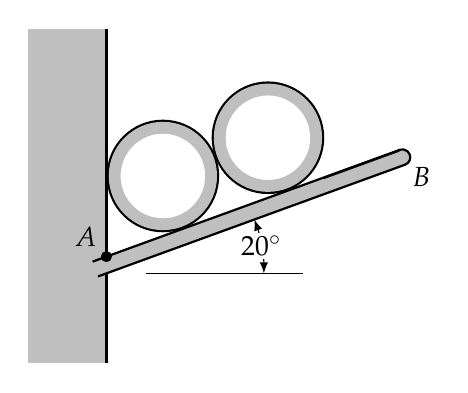
\begin{tikzpicture}[scale=\scale]
	\coordinate (A) at (0,0);
	\coordinate (B) at ($ (A)+(20:4) $);
	\coordinate (AA) at ($ (A)+(0, 0.1067) $);
	\coordinate (C) at ($ (A)+(0, 0.1067)+ (55:1.25) $);
	\coordinate (D) at ($ (C)+(20:1.42) $);

	
	\fill[gray!50] ($ (A)+(0,3) $) rectangle +(-1,-4.25);
	\draw[thick] ($ (A)+(0,3) $) --($ (A)+(0,-1.25) $);

	\draw[line width=0.2cm, gray!50, line cap=round] ($ (A)+(200:0.15) $) -- (B);

	% \Meme{A}{B}{SteelBlue3}{SteelBlue3}{SteelBlue3}{0.3}{0}{0}
	\draw[thick] ($ (A)+(110:0.1)+(200:0.15) $)--+(20:4.15);
	\draw[thick] ($ (A)+(-70:0.1)+(200:0.15) $)--+(20:4.15)arc(-70:130:0.1)--+(200:1);

	\fill (AA)circle(2pt)node[above left] {$ A $};
	\node[below right] at  (B) {$ B $};

	\draw[line width= 0.15cm] (C) circle (0.64cm);
	\draw[line width= 0.15cm,gray!50] (C) circle (0.6125cm);
	\draw[line width= 0.15cm] (D) circle (0.64cm);
	\draw[line width= 0.15cm,gray!50] (D) circle (0.6125cm);

	\draw ($ (A)-(0,0.1067)+(0.5,0) $) -- +(2,0);
	\draw[latex-latex] ($ (A)-(0,0.1067)+(2,0) $) arc(0:20:2)node[midway, fill=white, inner sep=0.4mm]{$ 20\deg $};


\end{tikzpicture}

  }
\end{textblock*}


\begin{textblock*}{4in}(1in, 2in)
  \centering
  \large
    The weight of each pipe bearing on $AB$:
    $$ W=78.5\,\mathsf{kg/m}\x 9.81\,\mathsf{m/s^2}\x 10\,\mathsf{m}/3=2.5670\,\mathsf{kN} $$    
\end{textblock*}

\begin{textblock*}{6.75in}(1in, 3in)
  \centering
  \large
  Add some labels, find some distances:\parm
  \mini[0.35]{
    \tikz{%color
      \coordinate (A) at (0,0);
      \coordinate (B) at ($ (A)+(20:4) $);
      \coordinate (D) at ($ (A)+(0, 0.1067)+ (55:1.25) $);
      \coordinate (C) at ($ (D)+(20:1.42) $);
      \coordinate (E) at ($ (D)!0.5!(C)+(110:.625) $);
      \coordinate (F) at ($ (C)+(-70:.64) $);
      \coordinate (G) at ($ (D)+(-70:.64) $);
      \coordinate (H) at ($ (D)+(180:.64) $);
      \draw[thick] ($ (A)+(0,2.5) $) --($ (A)+(0,-0.5) $);
      \draw[line width=0.2cm, gray!50, line cap=round] ($ (A)+(200:0.15) $) -- (B);
      \draw[line width= 0.15cm] (C) circle (0.64cm);
      \draw[line width= 0.15cm,gray!50] (C) circle (0.6125cm);
      \draw[line width= 0.15cm] (D) circle (0.64cm);
      \draw[line width= 0.15cm,gray!50] (D) circle (0.6125cm);
      \node[above, xshift=-2mm] at (A) {$ A $};
      \node[right] at (B) {$ B $};
      \node at (C) {$ C $};
      \node at (D) {$ D $};
      \node at (E) {$ E $};
      \node at ($ (F)+(-70:0.325) $) {$ F $};
      \node at ($ (G)+(-70:0.325) $) {$ G $};
      \node at ($ (H)+(-180:0.325) $) {$ H $};
    }
  }
  \mini[0.3]{
    \tikz{%color
      \coordinate (A) at (0,0);
      \coordinate (B) at ($ (A)+(20:8) $);
      \coordinate (D) at ($ (A)+(55:2.5) $);
      \coordinate (G) at ($ (D)+(-70:1.425) $);
      \coordinate (H) at ($ (D)+(180:1.425) $);

      \draw (A)--(D);
      \draw[thick] (D) circle (1.4cm);
      \draw (A)--($ (A)+(20:4 )$);
      \draw (A)--($ (A)!1.5!(H) $);
      \draw (D)--(G);
      \draw (D)--(H);
      \node[above] at (D) {$ D $};
      \node[left] at (H) {$ H $};
      \node[below] at (G) {$ G $};
      \node[below] at (A) {$ A $};
      \draw ($ (G)+(110:0.5) $)--++(20:0.5)--+(-70:0.5);
    }
  }
  \mini[0.3]{ 
    \begin{align*}
      \angle HAD &= \angle GAD = 35\deg \\
      \angle GAD &= 55\deg \\
      \frac{AG}{GD} &= \tan 55\deg \\
      AG &= \frac{508\,\text{mm}}{2}\tan 55\deg \\
       &=362.75\,\mathsf{mm} \\
      GF &= CD = 508\,\mathsf{mm}
    \end{align*}
  }
  \parb\centering
  {\bf Forces acting upon the upper (rightmost) pipe, $\bm C$}:\parb
  \mini[0.35]{    
      \centering
      \tikz{%color
        \coordinate (O) at (0,0);
        \coordinate (B) at ($ (A)+(20:4) $);
        % \coordinate (D) at ($ (A)+(0, 0.1067)+ (55:1.25) $);
        \coordinate (C) at ($ (D)+(20:1.42) $);
        \node[above] at (C) {$ C $};
        \draw[line width= 0.15cm] (C) circle (0.64cm);
        \draw[line width= 0.15cm,gray!50] (C) circle (0.6125cm);
        \draw[very thick, -latex] (C)--+(0,-1.5)node[below left]{$ 2.5670\,\mathsf{kN} $};
        \draw[very thick, latex-] ($ (C)+(210:0.64) $) --+(210:1.5)node[left]{$ R_E $};
        \draw[very thick, latex-] ($ (C)+(-70:0.64) $) --+(-70:1.5)node[right]{$ R_F $};
      } \parb
      \tikz{%color
        \coordinate (C) at (0,0);
        \draw[very thick, -latex] (C)--+(0,-1.75)node[below]{$ 2.5670\,\mathsf{kN} $};
        \draw[very thick, -latex] (C)--+(110:1.75)node[left]{$ R_F $};
        \draw[very thick, -latex] (C)--+(20:1.75)node[below right]{$ R_E $};
        \draw[latex-latex] ($ (C)+(0,-1.25) $)arc(-90:20:1.25) node[midway, fill=white] {$ 110\deg $};
        \draw[latex-latex] ($ (C)+(110:1.25) $)arc(110:270:1.25) node[midway, fill=white] {$ 160\deg $};
        \node[above,xshift=1mm] at (C) {$ C $};
      }
     
  }
  \normalsize  
  \hfill
   \mini[0.55]{ 
       
        This is now a simple concurrent forces problem, solved with simultaneous equations. Notice, however, that the direction of $R_F$ is perpendicular to the direction of $R_E$. \parb 
        If we choose axes $x'$ and $y'$, rotated $20\deg$ in the counter clockwise direction around $C$, then the direction of $R_E$ is the $x'$-axis and the direction of $R_F$ is the $y'$-axis. Now we can solve without simultaneous equations.\parb
        (Why bother complicating things? This will become a useful technique towards the end of the module and it's easy to introduce here.)
        \begin{align*}
          \Sigma F_{x'} &= R_E-2.5670\,\mathsf{kN}\cd\cos 70\deg =0 \\
          \Ra R_E &= 0.87800\,\mathsf{kN}\\\\
          \Sigma F_{y'} &= R_F-2.5670\,\mathsf{kN}\cd\cos 20\deg =0 \\
          \Ra R_F &= 2.4122\,\mathsf{kN}\\
        \end{align*}
        \vspace{-1cm}
      
    }
    \end{textblock*}

%%%%%%%%%%%%%%%%%%%%%%%%%%%%%%%%%%%%%%%%%%%%%%%%%%%%%%%%%%%%%%%%%%%%%%%%%%%%%%%%%%%%%%%%%%%%%%%%%%%%
% page 
%%%%%%%%%%%%%%%%%%%%%%%%%%%%%%%%%%%%%%%%%%%%%%%%%%%%%%%%%%%%%%%%%%%%%%%%%%%%%%%%%%%%%%%%%%%%%%%%%%%%
~\newpage

\begin{textblock*}{6.75in}(1in, 0.5in)
  \large\centering      
    {\bf Forces acting upon the lower (leftmost) pipe, $\bm D$:}
    \parb ~\parb
    \normalsize
    \mini[0.3]{
      \centering
      \tikz{%color
        \coordinate (D) at (0,0);
        \node[above] at (D) {$ D $};
        \draw[line width= 0.15cm] (D) circle (0.64cm);
        \draw[line width= 0.15cm,gray!50] (D) circle (0.6125cm);
        \draw[very thick, -latex] (C)--+(0,-1.5)node[below left]{$ 2.5670\,\mathsf{kN} $};
        \draw[very thick, latex-] ($ (C)+(20:0.64) $) --+(20:1.5)node[above]{$ 0.87800\,\mathsf{kN} $};
        \draw[very thick, latex-] ($ (C)+(180:0.64) $) --+(180:1.5)node[left]{$ R_H $};
        \draw[very thick, latex-] ($ (C)+(-70:0.64) $) --+(-70:1.5)node[right]{$ R_G $};
      }
      \parb
       \tikz{%color
        \coordinate (D) at (0,0);
        \draw[very thick, -latex] (D)--+(0,-1.75)node[below]{$ 2.5670\,\mathsf{kN} $};
        \draw[very thick, -latex] (D)--+(110:1.75)node[left]{$ R_G $};
        \draw[very thick, -latex] (D)--+(200:1.75)node[left]{$ 0.87800\,\mathsf{kN} $};
        \draw[very thick, -latex] (D)--+(0:1.75)node[right]{$ R_H $};
        \draw[latex-latex] ($ (D)+(270:1.25) $)arc(270:200:1.25) node[midway, fill=white, inner sep=1mm] {$ 70\deg $};
        \draw[latex-latex] ($ (D)+(0:1.25) $)arc(0:110:1.25) node[midway, fill=white] {$ 110\deg $};
        \node[xshift=-4mm, yshift=2mm] at (D) {$ D $};
        \draw ($ (D)+(0.325,0) $)--++(0,-0.325)--+(-0.325,0);
      }
    }    
    \hfill
    \mini[0.5]{      
        \vspace{3cm}
        \begin{align*}          
          \Sigma F_{y} &= R_G\cd\cos 20\deg -2.5670\,\mathsf{kN}-0.87800\,\mathsf{kN}\cd\cos 70\deg\\ &=0 \\
          \Ra R_G &= \frac{2.5670\,\mathsf{kN}+0.87800\,\mathsf{kN}\cd\cos 70\deg}{\cos 20\deg} \\
          \Ra R_G &= 3.0513\,\mathsf{kN}\\
        \end{align*}
        \vspace{-1cm}      
    }
    \parb 
   
    \def\scale{1.75}
    \tikz[scale=\scale]{%color
      \coordinate (A) at (0,0);
      \coordinate (B) at ($ (A)+(20:4) $);
      \coordinate (D) at ($ (A)+(0, 0.1067)+ (55:1.25) $);
      % \coordinate (C) at ($ (D)+(20:1.42) $);
      % \coordinate (E) at ($ (D)!0.5!(C)+(110:.625) $);
      \coordinate (F) at ($ (A)+(20:1) $);
      \coordinate (G) at ($ (A)+(20:2.5) $);
     
      \draw[line width=0.35cm, gray!50, line cap=round] ($ (A)+(200:0.15) $) -- (B);
     
      % \node[above, xshift=-2mm] at (A) {$ A $};
      \node[above right] at (B) {$ B $};      
      \node at ($ (F)+(-70:0.125) $) {$ F $};
      \node at ($ (G)+(-70:0.125) $) {$ G $};
      \node[xshift=0.25cm, yshift=-0.8cm] at (A) {$ R_a $};

      \fill (A) circle (1.5pt) node[xshift=-3mm]{$A $};
      \Couple{A}{black}{0.325}{0.625}
      \draw[ultra thick, -latex] (A)--+(0.75,0)node[below]{$ R_{Ax}$};
      \draw[ultra thick, -latex] (A)--+(0,0.75)node[left]{$ R_{Ay}$};
      \draw[ultra thick, latex-] (G)--+(110:1)node[left]{$3.0513\,\mathsf{kN}$};
      \draw[ultra thick, latex-] (F)--+(110:1)node[left]{$2.4122\,\mathsf{kN}$};

      \coordinate (AA) at ($ (A)+(-70:0.75) $);
      \coordinate (FF) at ($ (F)+(-70:0.75) $);
      \coordinate (GG) at ($ (G)+(-70:0.75) $);
      \draw[thin, gray] (AA)--+(-70:0.5);
      \draw[thin, gray] (FF)--+(-70:0.5);
      \draw[thin, gray] (GG)--+(-70:0.5);
      \draw[thin, gray] ($ (A)+(0:0.875) $)--+(0:1.25);
      \draw[thin] ($ (A)+(20:0.5) $)--+(20:2.5);

      \draw[latex-latex]  ($ (AA)+(-70:0.25) $) -- ($ (FF)+(-70:0.25) $) node[fill=white, midway, rotate=-45] {$ 362.75\,\mathsf{mm}$};
      \draw[latex-latex]  ($ (FF)+(-70:0.25) $) -- ($ (GG)+(-70:0.25) $) node[fill=white, midway,sloped] {$ 508\,\mathsf{mm}$};
      \draw[latex-latex]  ($ (A)+(-0:1.75) $) arc(0:20:1.75) node[midway, fill=white, inner sep=1mm] {$ 20\deg $};

      \draw (F)--++(110:0.2)--++(20:0.2)--+(-70:0.2);
      \draw (G)--++(110:0.2)--++(20:0.2)--+(-70:0.2);
    }

    \begin{align*}
      \Sigma M_A &= R_a-2.4122\,\mathsf{kN}\cd 362.75\,\mathsf{mm} -3.0513\,\mathsf{kN}\cd 870.75\,\mathsf{mm}=0 \Ra R_a = 3531.9\,\mathsf{kN\cd mm} = 3.5319\,\mathsf{kN\cd m} \\[0.25em]
      \Sigma F_x &= R_{Ax}+2.4122\,\mathsf{kN}\cd\sin 20\deg +3.0513\,\mathsf{kN}\cd\sin 20\deg=0 \Ra R_{Ax} = -1.8686\,\mathsf{kN} \\[0.25em]
      \Sigma F_x &= R_{Ay}-2.4122\,\mathsf{kN}\cd\cos 20\deg -3.0513\,\mathsf{kN}\cd\cos 20\deg=0 \Ra R_{Ay} = 5.1340\,\mathsf{kN}
    \end{align*}
    \mini[0.2]{
      \tikz[scale=0.75]{%color
        \coordinate (O) at (0,0);
        \draw[-latex, thick] (O) -- +(-1.86,0)node[below]{$1.8686\,$\textsf{kN}};
        \draw[-latex, thick] (O) -- +(0,5)node[above]{5.1340\,\textsf{kN}};
        \draw[-latex, ultra thick] (O) -- +(-1.86,5)node[left]{$ R_A $};
        \node at (-0.5,0.35){$ \theta $};
      }
    }
    \hfill
    \mini[0.75]{
      \begin{align*}
        R_A &= \sqrt{(1.8686\,\textsf{kN})^2+(5.1340\,\textsf{kN})^2} = 5.4635\,\textsf{kN}\\[0.25em]
        \theta &= \tan^{-1}\left[\frac{5.1340\,\textsf{kN}}{1.8686\,\textsf{kN}}\right] = 70\deg
      \end{align*}
      \parb\large
      The reaction at $A$ is $\underline{\bm{5.46\,\mathsf{kN}}}$ at $\underline{\bm{110\deg}}$ counter-clockwise from the positive $x$-axis. The reacting moment at $A$ is $\underline{\bm{3.53\,\mathsf{kN\cd m}}}$
    }

\end{textblock*}
     
%%%%%%%%%%%%%%%%%%%%%%%%%%%%%%%%%%%%%%%%%%%%%%%%%%%%%%%%%%%%%%%%%%%%%%%%%%%%%%%%%%%%%%%%%%%%%%%%%%%
% page 12
%%%%%%%%%%%%%%%%%%%%%%%%%%%%%%%%%%%%%%%%%%%%%%%%%%%%%%%%%%%%%%%%%%%%%%%%%%%%%%%%%%%%%%%%%%%%%%%%%%%%

~\newpage
\begin{textblock*}{2.5in}(1in, 0.1in)
	\cbox{
		\underbar{\bf Exercise 4:} 
		A section of smooth pipe, centred at $O$, has a diameter of $457\,\textsf{mm} $ and a mass of $186\,\textsf{kg}$. It is secured by vertical structural member $AB$, hinged with a pinned connection at $A$ and held in place by chain $BC$.\parb
    Determine the tension in the chain, and the reaction at $A$.	
	}
\end{textblock*}
\begin{textblock*}{3.75in}(4.025in, 0.1in)
	\cbox{
    \centering
    \def\scale{0.75}
    \tikz[scale=\scale,decoration={
		markings,% switch on markings
		mark=% actually add a mark
		between positions 0 and 1 step 9pt
		with
		{
			\begin{scope}[scale=0.75]
				\draw[black, very thick] (0pt,-2pt) -- ++(4pt,0) arc(-90:90:2pt) -- ++(-4pt,0pt) arc(90:270:2pt) -- cycle;
				\draw[black,very thick] (-8pt,0) -- (0pt,0);
			\end{scope}
		}
	}]{
	\coordinate (A) at (0,0);
	\coordinate (B) at (0,5);
	\coordinate (BB) at (0,6);
	\coordinate (C) at (8,5);
	\coordinate (Cleft) at (7.5,5);

	\coordinate (AA) at ($ (A)+(212:1.5)$);
	
	\coordinate (AAA) at ($ (A)+(32:0.175)$);
	\coordinate (CC) at ($ (C)+(32:1)$);
	\coordinate (O) at ($ (AAA)+(61:3)$);
	
	
	\path[postaction={decorate}] ($ (B)+(0.5,0) $) -- (Cleft);
	\PC[32]{Cleft}{gray!30}{black}{0.5}{0.25};
	\draw[ultra thick] (AA)--(CC);
	\fill[fill=gray!60](AA)--(CC)--++(-58:1) to [out=-115, in=45]++(212:11.934)--cycle;
	\PC{A}{gray!30}{black}{0.5}{0.25};
	
	\filldraw[fill=gray!30] ($ (B)+(0,0.25) $) --++(-30:0.5)--+(210:0.5);
	\Meme{A}{BB}{gray!30}{gray!30}{black}{0.325}{0.1}{0.2}

	
	\draw[line width=2mm, gray] (O) circle (1.3cm);
	\draw[thick] (O) circle (1.4cm);
	
	\node[xshift=-1cm, yshift=-0.3cm] at (C) { $ 32\deg $};
	\node[xshift=0.5cm, yshift=0.6cm] at (A) { $ 58\deg $};
	
	\draw ($ (A)-(1,0) $)--+(-1,0);
	\draw ($ (B)-(1,0) $)--+(-1,0);

	\fill (A) circle (1.5pt) node [xshift=-0.325cm,yshift=0.25cm] {\Large $A$};
	\fill (O) circle (1.5pt)node[above] {$ O $};
	\node[above,outer sep=1mm] at (C)   {\Large $C$};
	\fill (B) circle (1.5pt) node [left,outer sep=1mm] {\Large $B$};

	\draw[latex-latex]($ (A)-(1.5,0) $) -- ($ (B)-(1.5,0) $)node[midway, fill=white]{$ 625\,\text{mm}$};
}

  }
\end{textblock*} 

\begin{textblock*}{2.5in}(1in, 2.25in)
  \centering
  The weight of the pipe is:\pars
  $ W = 186\x9.81\,\textsf{N} = 1824.7\,\textsf{N}$ 
  \parb
	Forces acting on the pipe:\parm
  \tikz[scale=0.75]{%color
    \draw[ultra thick] (0,0) circle (1.3cm);
    \draw[very thick, -latex] (0,0)--+(0,-2)node[below]{$ 1.8247\,\textsf{kN} $};
    \draw[very thick, latex-] (-1.3,0)--+(-1,0)node[below]{$ R_D $};
    \draw[very thick, latex-] (-58:1.3)--+(-58:1)node[right]{$ R_E $};
  }
  \parm
  Free body diagram:
  \parm
    \tikz[scale=0.75]{%color
    \draw[very thick, -latex] (0,0)--+(0,-2)node[below]{$ 1.8247\,\textsf{kN} $};
    \draw[very thick, -latex] (0,0)--+(1.5,0)node[below]{$ R_D $};
    \draw[very thick, -latex] (0,0)--+(122:2)node[right]{$ R_E $};
    \draw[thin, gray] (-0.75,0)--+(-1,0);
    \draw[latex-latex] (-1.25,0)arc(180:122:1.25)node[midway, fill=white,inner sep=0.3mm]{\small$ 58\deg $};
  }
  \parm
  Determine the length of the moment-arm, $AD$, where the pipe bears on the vertical member.
  \parb
  \tikz[scale=1.25]{%color
    \coordinate (O) at (0,0);
    \coordinate (D) at ($ (O)+(-1.371,0) $);
    \coordinate (A) at ($ (D)+(0,-2.4733) $);
    \coordinate (E) at ($ (O)+(-58:1.371) $);
    \draw (A)--(D);
    \draw (A)--(O);
    \draw (A)--(E);
    \draw (O)--(E)node[midway, above, sloped]{\footnotesize $ 228.5\,\textsf{mm} $};
    \draw (O)--(D)node[midway, above]{\footnotesize $ 228.5\,\textsf{mm} $};;
    \draw[very thick] (O) circle (1.371cm);
    \node[below] at (A) {$ A $};
    \node[right, xshift=0.125cm] at (E) {$ E $};
    \node[above] at (O) {$ O $};
    \node[above left] at (D) {$ D $};
    \node at ($ (O)+(208:0.35) $) {\footnotesize $ 61\deg $};
    \node at ($ (O)+(-88:0.45) $) {\footnotesize $ 61\deg $};
    \node at ($ (A)+(73:0.75) $) {\footnotesize $ 29\deg $};
    \node at ($ (A)+(45:0.75) $) {\footnotesize $ 29\deg $};
    \node at ($ (A)+(16:0.75) $) {\footnotesize $ 32\deg $};
    \draw[thin, gray]  ($ (A)+(0:0) $)--($ (A)+(0:0.95) $);
  }
\end{textblock*}

\begin{textblock*}{3.5in}(3.5in, 4.5in)
  \begin{align*}
    \Sigma F_y &= R_E\cd\sin 58\deg -1.8247\,\text{kN} = 0 \\[0.25em] 
    \Ra R_E &= 2.1516\,\textsf{kN} \\\\
    \Sigma F_x &= R_D-(2151.6\,\textsf{kN})\cd\cos 58\deg = 0 \\[0.25em] 
    \Ra R_D &= 1.1402\,\textsf{kN}
  \end{align*}
\end{textblock*}
\begin{textblock*}{3.5in}(3.5in, 7.5in)
  \begin{align*}
    \frac{AD}{228.5\,\textsf{mm}} &= \tan 61\deg \Ra AD = 412.22\,\textsf{mm}
   \end{align*}
\end{textblock*}
  
 
%%%%%%%%%%%%%%%%%%%%%%%%%%%%%%%%%%%%%%%%%%%%%%%%%%%%%%%%%%%%%%%%%%%%%%%%%%%%%%%%%%%%%%%%%%%%%%%%%%%
% page 13
%%%%%%%%%%%%%%%%%%%%%%%%%%%%%%%%%%%%%%%%%%%%%%%%%%%%%%%%%%%%%%%%%%%%%%%%%%%%%%%%%%%%%%%%%%%%%%%%%%%
~\newpage
\begin{textblock*}{2.5in}(1in, 1in)
  \centering
  \tikz[scale=1]{%color
    \coordinate (A) at (0,0);
	  \coordinate (B) at (0,5);
	  \coordinate (D) at ($ (A)!0.66!(B) $);
    \draw[line width = 0.5cm, gray!50, line cap = round] (A)--(B);
    \draw[latex-, ultra thick] (D)--+(1.5,0)node[right]{$ 1.1402\,\textsf{kN} $};
    \draw[ultra thick, -latex]  (A)--+(1.5,0)node[right]{$ R_{Ax} $};
    \draw[ultra thick, -latex]  (A)--+(0, 1.5)node[left]{$ R_{Ay} $};
    \draw[ultra thick, -latex]  (B)--+(1.5, 0)node[right]{$ T_{BC} $};

    \node[xshift=-0.5cm] at (A) {$ A $};
    \node[xshift=-0.5cm] at (D) {$ D $};
    \node[xshift=-0.5cm] at (B) {$ B $};

    \draw[latex-latex] ($ (A)+(0.75,0) $) --  ($ (D)+(0.75,0) $) node[midway, xshift=0.5cm, fill=white] {$ 412.22\,\textsf{mm} $};
    \draw[latex-latex] ($ (A)+(-1.75,0) $) --  ($ (B)+(-1.75,0) $) node[midway,fill=white] {$ 625\,\textsf{mm} $};

    \draw[thin, gray] ($ (A)-(1,0) $) -- ($ (A)-(3,0) $);
    \draw[thin, gray] ($ (B)-(1,0) $) -- ($ (B)-(3,0) $);

  }
 
\end{textblock*}

\begin{textblock*}{3.5in}(4in, 1in)
  \begin{align*}
    \Sigma M_A &= (1.1402\,\textsf{kN})\cd(412.22\,\textsf{mm})-(625\,\textsf{mm})T_{BC} = 0 \\[0.25em]
    \Ra T_{BC} &= 0.75202\,\textsf{kN}\\\\
    \Sigma F_x &= R_{Ax}-1.1402\,\textsf{kN}+0.75202\,\textsf{kN} = 0 \\[0.25em]
    \Ra R_{Ax} &= 0.38818\,\textsf{kN} \\\\
    \Sigma F_y &= R_{Ay} = 0 \\[0.25em]    
  \end{align*}
\end{textblock*}
\begin{textblock*}{6in}(1.5in, 3.5in)
   \parb\large\centering
      The tension in the chain between $B$ and $C$  is $\underline{\bm{0.752\,\mathsf{kN}}}$. 
      
      \parb
      
      The reaction at $A$ is $\underline{\bm{0.388\,\mathsf{kN}}}$ in the direction of the positive $x$-axis
\end{textblock*}

%%%%%%%%%%%%%%%%%%%%%%%%%%%%%%%%%%%%%%%%%%%%%%%%%%%%%%%%%%%%%%%%%%%%%%%%%%%%%%%%%%%%%%%%%%%%%%%%%%%
% page 13
%%%%%%%%%%%%%%%%%%%%%%%%%%%%%%%%%%%%%%%%%%%%%%%%%%%%%%%%%%%%%%%%%%%%%%%%%%%%%%%%%%%%%%%%%%%%%%%%%%%%

~\newpage
\begin{textblock*}{2.5in}(1in, 0.1in)
	\cbox{
		\underbar{\bf Example 8:} 
      \pars
			Soil exerts a trapezoidal distributed load on the bottom of the footing $AB$. \pars Determine the values of $\omega_1$ and $\omega_2$ that support the column loadings in static equilibrium.			
	}
\end{textblock*}
\begin{textblock*}{3.75in}(4.025in, 0.1in)
	\cbox{
    \centering
    \def\scale{0.75}
    \tikz[scale=\scale]{
  \coordinate (A) at (0,0);
  \coordinate (C) at (1,0);
  \coordinate (D) at (2.2,0);
  \coordinate (E) at (5.6,0);
  \coordinate (B) at (8,0);

  \fill[gray!50] ($(A)+(-2,0)$) rectangle ($ (B)+(2,-3.75) $);
  
  \node[below left] at (A) {$ A $};
  \node[below right] at (B) {$ B $};

  \fill[gray!30] ($ (C)-(0.25,0) $) rectangle ($ (C)+(0.25,4) $);
  \draw[ very thick] ($ (C)+(-0.25,0) $) rectangle ($ (C)+(-0.25,4) $);
  \draw[ very thick] ($ (C)+(0.25,0) $) rectangle ($ (C)+(0.25,4) $);
  \fill[gray!30] ($ (D)-(0.25,0) $) rectangle ($ (D)+(0.25,4) $);
  \draw[ very thick] ($ (D)+(-0.25,0) $) rectangle ($ (D)+(-0.25,4) $);
  \draw[ very thick] ($ (D)+(0.25,0) $) rectangle ($ (D)+(0.25,4) $);
  \fill[gray!30] ($ (E)-(0.25,0) $) rectangle ($ (E)+(0.25,4) $);
  \draw[ very thick] ($ (E)+(-0.25,0) $) rectangle ($ (E)+(-0.25,4) $);
  \draw[ very thick] ($ (E)+(0.25,0) $) rectangle ($ (E)+(0.25,4) $);

  \draw[very thick, latex-] ($ (C)+(0,4) $) --+ (0,2)node[above]{\small$ 200\,\textsf{kN} $};
  \draw[very thick, latex-] ($ (D)+(0,4) $) --+ (0,1.4)node[above]{\small$ 140\,\textsf{kN} $};
  \draw[very thick, latex-] ($ (E)+(0,4) $) --+ (0,1.6)node[above]{\small$ 160\,\textsf{kN} $};

  \draw[thin, gray] ($ (A)+(0,0.5) $) -- ($ (A)+(0,5.5) $);
  \draw[thin, gray] ($ (B)+(0,0.5) $) -- ($ (B)+(0,5.5) $);

  \draw[latex-latex] ($ (A)+(0,4.75) $) -- ($ (C)+(0,4.75) $) node[midway, fill=white, yshift=0.157cm,inner sep=0mm] {\scriptsize $ 1\,\textsf{m}$};
  \draw[latex-latex] ($ (C)+(0,4.75) $) -- ($ (D)+(0,4.75) $) node[midway, fill=white, yshift=0.157cm,inner sep=0mm] {\scriptsize $ 1.2\,\textsf{m}$};
  \draw[latex-latex] ($ (D)+(0,4.75) $) -- ($ (E)+(0,4.75) $) node[midway, fill=white, yshift=0.157cm,inner sep=0mm] {\scriptsize $ 3.4\,\textsf{m}$};
  \draw[latex-latex] ($ (E)+(0,4.75) $) -- ($ (B)+(0,4.75) $) node[midway, fill=white, yshift=0.157cm,inner sep=0mm] {\scriptsize $ 2.4\,\textsf{m}$};

  \begin{scope}[yshift=-0.75cm]
    \coordinate (TL) at (0,1);
    \coordinate (TR) at (8,2);
    \coordinate (base) at (0,0);
    \DLdown[180]{TL}{TR}{base}{gray!50}{black}{10}{0.4}{5};
  \end{scope}

  \filldraw[fill=gray!15] (A) rectangle ($ (B)+(0,-0.75) $);
  \draw [thick] ($ (A)+(-2,0) $) -- ($ (B)+(2,0) $);
  \node at (-0.5,-3) {$ \omega_1 $};
  \node at (8.5,-2) {$ \omega_2 $};


}
  }
\end{textblock*} 

\begin{textblock*}{\textwidth}(1in, 4in)
	\centering
  \tikz{%color
    \coordinate (A) at (0,0);
    \coordinate (C) at (1,0);
    \coordinate (D) at (2.2,0);
    \coordinate (E) at (5.6,0);
    \coordinate (B) at (8,0);
    \coordinate (O) at (8/3,0);


    \draw[line width = 0.5cm, line cap = round, gray!20](A)--(B);
    \draw[thin](A)--(B);
    \fill (A) circle (1.5pt) node[left]{\large $ A $};
    \fill (B) circle (1.5pt) node[right]{\large $ B $};
    \fill (O) circle (1.5pt) node[above]{\large $ O $};

    \draw[very thick, latex-] (C) --+ (0,2)node[above]{\small$ 200\,\textsf{kN} $};
    \draw[very thick, latex-] (D) --+ (0,1.4)node[above]{\small$ 140\,\textsf{kN} $};
    \draw[very thick, latex-] (E) --+ (0,1.6)node[above]{\small$ 160\,\textsf{kN} $};

    \draw[thin, gray] ($ (A)+(0,0.325) $) -- ($ (A)+(0,1.125) $);
    \draw[thin, gray] ($ (B)+(0,0.325) $) -- ($ (B)+(0,1.125) $);
    \draw[thin, gray] ($ (A)+(0,-0.325) $) -- ($ (A)+(0,-1.125) $);
    \draw[thin, gray] ($ (B)+(0,-0.325) $) -- ($ (B)+(0,-1.125) $);

    \draw[latex-latex] ($ (A)+(0,.75) $) -- ($ (C)+(0,.75) $) node[midway, fill=white, yshift=0.157cm,inner sep=0mm] {\footnotesize $ 1\,\textsf{m}$};
    \draw[latex-latex] ($ (C)+(0,.75) $) -- ($ (D)+(0,.75) $) node[midway, fill=white, yshift=0.157cm,inner sep=0mm] {\footnotesize $ 1.2\,\textsf{m}$};
    \draw[latex-latex] ($ (D)+(0,.75) $) -- ($ (E)+(0,.75) $) node[midway, fill=white, yshift=0.157cm,inner sep=0mm] {\footnotesize $ 3.4\,\textsf{m}$};
    \draw[latex-latex] ($ (E)+(0,.75) $) -- ($ (B)+(0,.75) $) node[midway, fill=white, yshift=0.157cm,inner sep=0mm] {\footnotesize $ 2.4\,\textsf{m}$};
    \draw[latex-latex] ($ (A)+(0,-.75) $) -- ($ (O)+(0,-.75) $) node[midway, fill=white, yshift=0.157cm,inner sep=0mm] {\footnotesize $ 2.6667\,\textsf{m}$};
    \draw[latex-latex] ($ (O)+(0,-.75) $) -- ($ (4,0)+(0,-.75) $) node[midway, fill=white, yshift=0.157cm,inner sep=0mm] {\footnotesize $ 1.3333\,\textsf{m}$};
    \draw[latex-latex] ($ (4,0)+(0,-.75) $) -- ($ (B)+(0,-.75) $) node[midway, fill=white, yshift=0.157cm,inner sep=0mm] {\footnotesize $ 4.0\,\textsf{m}$};

    \draw[very thick, latex-] (4,0)--+(0,-1.5) node[below]{$ 8\cd \omega_2 $};
    \draw[very thick, latex-] (8/3,0)--+(0,-1) node[below]{$ 4\cd(\omega_1- \omega_2) $};
  }
  \parm\raggedright
  \cmini{
    We could start by taking moments about $A$ to get an expression with $\omega_1$ and $\omega_2$. Then do the same with moments about $B$. And get a system of two equations in two unknowns.\parb
    Or we could take moments about $O$ and not have to deal with simultaneous equations!\parb
    \underline{\bf Note:} The $8\cd\omega_2$ is in \textsf{kN} where the $8$ is in \textsf{m} and the $\omega_2$ is in \textsf{kN/m}. Similarly for $4(\omega_1-\omega_2)$.
  }
  
  \begin{align*}
    \Sigma M_O &= (8\,\textsf{m})\omega_2\cd(1.3333\,\text{m}) + (140\,\textsf{kN})(0.46670\,\text{m})+ (200\,\textsf{kN})(1.6667\,\text{m})- (160\,\textsf{kN})(2.9333\,\text{m}) \\[0.25em]
    &= (10.644\,\mathsf{m^2})\omega_2  -70.650\,\mathsf{kN\cd m} = 0 \\[0.25em]
    \Ra \omega_2 &= 6.6236\,\textsf{kN/m} \\\\
    \Sigma F_y &= (8\,\textsf{m})\omega_2 +(4\,\textsf{m})(\omega_1-\omega_2) - 500\,\text{kN} \\[0.25em]
    &= (4\,\textsf{m})\omega_1 +(4\,\textsf{m})\omega_2 -500\,\textsf{kN} = (4\,\textsf{m})\omega_1 +26.494\,\textsf{kN} -500\,\textsf{kN} =0 \\[0.25em]
    \Ra \omega_1 &= \frac{473.51\,\textsf{kN}}{4\,\textsf{m}}  = 118.38\,\textsf{kN/m}
  \end{align*}
  \large\centering
      \begin{align*}
        \omega_1 &= \underline{118\,\textsf{kN/m}}\\
        \omega_2 &= \underline{6.62\,\textsf{kN/m}}\\
      \end{align*}
\end{textblock*}

%%%%%%%%%%%%%%%%%%%%%%%%%%%%%%%%%%%%%%%%%%%%%%%%%%%%%%%%%%%%%%%%%%%%%%%%%%%%%%%%%%%%%%%%%%%%%%%%%%%
% page 14
%%%%%%%%%%%%%%%%%%%%%%%%%%%%%%%%%%%%%%%%%%%%%%%%%%%%%%%%%%%%%%%%%%%%%%%%%%%%%%%%%%%%%%%%%%%%%%%%%%%%

~\newpage
\begin{textblock*}{2.5in}(1in, 0.1in)
	\cbox{
		\underbar{\bf Example 9:} 
      \pars
			Determine the reactions at $D$ and $E$.		
	}
\end{textblock*}
\begin{textblock*}{3.75in}(4.025in, 0.1in)
	\cbox{
    \centering
    \def\scale{0.65}
    % !TEX root = ../../Beamer/06EquilibriumOfRigidBodies/06ERB.tex

\makeatletter
\providecommand{\gettikzxy}[3]{%
	\tikz@scan@one@point\pgfutil@firstofone#1\relax
	\edef#2{\the\pgf@x}%
	\edef#3{\the\pgf@y}%
}
\makeatother

\begin{tikzpicture}[scale=\scale]
	

	\coordinate (A) at (0, 0);
	\coordinate (B) at (3, 0);
	\coordinate (C) at (7, 0);
	\coordinate (D) at (10, 1.25);
	\coordinate (E) at (10, -3.5);
	\coordinate (F) at (7, -3.5);
	\coordinate (G) at (3, -3.5);

	\fill[myGray] ($ (E)+(0.75,-1.25) $) rectangle ($ (D)+(1.5,2) $);
	\draw[black, line width=0.2mm] ($ (E)+(0.75,-1.25) $) -- ($ (D)+(0.75,2) $);

	\PC[90]{D}{myGray}{black}{0.75}{0.2}
	\PC[90]{E}{myGray}{black}{0.75}{0.2}

	\gettikzxy{(A)}{\Ax}{\Ay};
	\gettikzxy{(B)}{\Bx}{\By};

	\Meme{A}{B}{myGray3}{myGray3}{black}{0.35}{0.125}{0.2}
	\Meme{C}{D}{myGray3}{myGray3}{black}{0.35}{0.125}{0.2}
	\Meme{A}{G}{myGray3}{myGray3}{black}{0.35}{0.125}{0.2}
	\Meme{F}{G}{myGray3}{myGray3}{black}{0.35}{0.125}{0.2}
	\Meme{F}{E}{myGray3}{myGray3}{black}{0.35}{0.125}{0.2}
	\Meme{C}{G}{myGray3}{myGray3}{black}{0.35}{0.125}{0.2}
	\Meme{C}{E}{myGray3}{myGray3}{black}{0.35}{0.125}{0.2}
	\Meme{C}{B}{myGray3}{myGray3}{black}{0.35}{0.125}{0.2}
	\Meme{C}{F}{myGray3}{myGray3}{black}{0.35}{0.125}{0.2}
	\Meme{B}{G}{myGray3}{myGray3}{black}{0.35}{0.125}{0.2}

	\gettikzxy{(C)}{\Cx}{\Cy};
	\gettikzxy{(E)}{\Ex}{\Ey};
	\gettikzxy{(D)}{\Dx}{\Dy};

	\draw[thin] ($ (A)+(0,0.5) $) -- +(0,2.75);
	\draw[thin] ($ (B)+(0,0.5) $) -- +(0,2.75);
	\draw[thin] ($ (C)+(0,0.5) $) -- +(0,2.75);
	\draw[thin] ($ (D)+(0,0.5) $) -- +(0,1.5);
	\draw[thin] ($ (E)+(1,0) $) -- (13, \Ey);
	\draw[thin] ($ (C)+(0.75,0) $) -- (13, \Cy);
	\draw[thin] ($ (D)+(1,0) $) -- (13, \Dy);

	\draw[line width=0.75mm, black, -latex] (A) -- +(0,-2.5) node[below] {\large {$ 30$ kN}};

	\draw[ latex-latex] ([yshift=2.5cm]A) -- node[fill=white]{\small $3.00\textsf{ m}$}([yshift=2.5cm]B);
	\draw[ latex-latex] ([yshift=2.5cm]B) -- node[fill=white]{\small $4.00\textsf{ m}$}([yshift=2.5cm]C);
	\draw[ latex-latex] ([yshift=2.5cm]C) -- node[fill=white]{\small $3.00\textsf{ m}$}([yshift=1.25cm]D);
	\draw[ latex-latex] (12.5, \Dy) -- node[fill=white, inner sep=0.5mm]{\small $1.25\textsf{ m}$}(12.5, \Cy);
	\draw[ latex-latex] (12.5, \Cy) -- node[fill=white, inner sep=0.5mm]{\small $3.50\textsf{ m}$}(12.5, \Ey);

	\fill (A) circle (2.5pt) node[above left, inner sep=2mm] {\large $A$};
	\fill (B) circle (2.5pt) node[above left, inner sep=2mm] {\large $B$};
	\fill (C) circle (2.5pt) node[above left, inner sep=2mm] {\large $C$};
	\fill (D) circle (2.5pt) node[above left, inner sep=2mm] {\large $D$};
	\fill (E) circle (2.5pt) node[below, inner sep=2mm] {\large $E$};
	\fill (F) circle (2.5pt) node[below, inner sep=2mm] {\large $F$};
	\fill (G) circle (2.5pt) node[below , inner sep=2mm] {\large $G$};

\end{tikzpicture}

  }
\end{textblock*} 

\begin{textblock*}{2.5in}(1in, 1.25in)
	\underline{\bf{Note:}} We cannot usually solve a system with two pinned connections because there are two unknowns. In this case, though, $CD$ is a two-force member so we know its direction and the only unknown at $D$ is the magnitude of the direction. We can treat $CD$ as we would a cable or a strut.
\end{textblock*}

\begin{textblock*}{6.75in}(1in, 3in)
  \center
	\tikz[scale=0.625]{%color
    \coordinate (A) at (0, 0);
    \coordinate (B) at (3, 0);
    \coordinate (C) at (7, 0);
    \coordinate (D) at (10, 1.25);
    \coordinate (E) at (10, -3.5);
    \coordinate (F) at (7, -3.5);
    \coordinate (G) at (3, -3.5);
    \fill[myGray3] (A)--(C)--(D)--(E)--(G)--cycle;
    \draw[ultra thick, -latex] (D)--+(22.62:1.75)node[above]{$ R_D $};
    \draw[ultra thick, -latex] (E)--+(0:2)node[below]{$ R_{Ex} $};
    \draw[ultra thick, -latex] (E)--+(90:1.5)node[left]{$ R_{Ey} $};
    \draw[ultra thick, -latex] (A)--+(-90:1.5)node[left]{$ 30\,\textsf{kN} $};
    \fill (A) circle (2.5pt) node[above left, inner sep=2mm] {\large $A$};
    \fill (D) circle (2.5pt) node[above left, inner sep=2mm] {\large $D$};
	  \fill (E) circle (2.5pt) node[below, inner sep=2mm] {\large $E$};
    \draw[thin] ($ (A)+(0,0.5) $) -- +(0,2.75);
    \draw[thin] ($ (D)+(0,0.5) $) -- +(0,1.5);
    \draw[thin] ($ (D)+(0.5,0) $) -- +(1,0);
    \draw[ latex-latex] ([yshift=2.5cm]A) -- node[fill=white]{\small $10.00\textsf{ m}$}([yshift=1.25cm]D);
    \draw[ latex-latex] ([xshift=1cm]D) -- node[fill=white]{\small $4.75\textsf{ m}$}([xshift=1cm]E);
    \draw[latex-latex] ($ (D)+(202.62:1.5) $) arc(202.62:270:1.5)node[midway, fill=myGray3, rotate=45] {\footnotesize $ 67.380\deg $};
  }
  \begin{align*}
    \Sigma M_E &= (30\,\textsf{kN})\cd (10.00\,\textsf{m}) -R_D\cd (4.75\,\textsf{m}\cd \sin 67.380\deg) = 0 \\[0.25em]
    \Ra R_D &= \frac{(30\,\textsf{kN})\cd (10.00\,\textsf{m})}{4.75\,\textsf{m}\cd \sin 67.380\deg}\\[0.25em]
    &= 68.421\,\textsf{kN}\\\\
    \Sigma F_x &= R_{Ex}+(68.421\,\textsf{kN})\cd \sin 67.380\deg = 0 \\[0.25em]
    \Ra R_{Ex} &= -63.158\,\textsf{kN} \\\\
    \Sigma F_y &= R_{Ey}+(68.421\,\textsf{kN})\cd \cos 67.380\deg - 30\,\textsf{kN}= 0 \\[0.25em]
    \Ra R_{Ey} &= 3.6481\,\textsf{kN}
  \end{align*}
  \pars
  \tikz{%color
    \draw[very thick, -latex] (0,0)--+(0,1)node[above]{$ 3.6481\,\textsf{kN} $};
    \draw[very thick, -latex] (0,0)--+(-5,0)node[below]{$ 63.158\,\textsf{kN} $};
    \draw[very thick, -latex, gray] (0,0)--+(-5,1)node[below]{$ R_E $};
    \node at (-2,0.2) {$ \theta $};
  }
  \pars
  \begin{align*}
    R_E &= \sqrt{(-63.158\,\textsf{kN})^2+(-3.6481\,\textsf{kN})^2} = 63.263\,\textsf{kN}\\[0.25em]
    \theta &= \tan^{-1}\left[\frac{3.6481}{63.158}\right] = 3.3058\deg
  \end{align*}

  \parb\large\centering
      The reaction at $E$ is $\underline{\bm{68.4\,\mathsf{kN}}}$ at  $\underline{\bm{22.6\deg}}$, measured counter-clockwise from the positive $x$-axis.
      
      \parm
      
      The reaction at $D$ is $\underline{\bm{63.3\,\mathsf{kN}}}$ at  $\underline{\bm{177\deg}}$, measured counter-clockwise from the positive $x$-axis.
\end{textblock*}

%%%%%%%%%%%%%%%%%%%%%%%%%%%%%%%%%%%%%%%%%%%%%%%%%%%%%%%%%%%%%%%%%%%%%%%%%%%%%%%%%%%%%%%%%%%%%%%%%%%
% page 15
%%%%%%%%%%%%%%%%%%%%%%%%%%%%%%%%%%%%%%%%%%%%%%%%%%%%%%%%%%%%%%%%%%%%%%%%%%%%%%%%%%%%%%%%%%%%%%%%%%%%

~\newpage
\begin{textblock*}{2.5in}(1in, 0.1in)
	\cbox{
		\underbar{\bf Exercise 5:} 
      \pars
			Determine the reactions at $A$ and $D$.		
	}
\end{textblock*}
\begin{textblock*}{3.75in}(4.025in, 0.1in)
	\cbox{
    \centering
    \def\scale{0.65}
    

\begin{tikzpicture}[scale=\scale]

	\coordinate (A) at (0, 0);
	\coordinate (AA) at ($(A)+(1.5,2)$);
	\coordinate (B) at (4, 0);
	\coordinate (C) at (6, 0);
	\coordinate (CC) at ($(C)+(0,1.55*0.25)$);
	\coordinate (D) at (4,3.5);
	\coordinate (E) at (0,-3);
	\coordinate (base) at ($(A)+(0,0.3875)$);

	\fill[gray] ($ (A)+(-0.75,4) $) rectangle ($ (E)+(-1.75,-2) $);
	\draw[black, thick] ($ (A)+(-0.75,4) $) -- +(0, -9);

	\DL{base}{D}{base}{myGray4}{black}{8}{0.25}{5}
	\DL{CC}{D}{base}{myGray4}{black}{4}{0.25}{5}


	\fill[gray!60] ($ (A)+(-0.25,-0.3875) $) rectangle ($ (C)+(0,0.3875) $);
	\draw[ultra thick] ($ (A)+(-0.25,-0.3875) $) -- ++(6.25,0);
	\draw[ultra thick] ($ (A)+(-0.25,0.3875) $) -- ++(6.25,0);



	\filldraw [fill=gray!60, draw=black, line width=0.35mm] (0,-2.75) arc [start angle=-90, end angle=0, x radius=3.75cm, y radius=2.75cm]arc(180:0:0.25) arc[start angle=0, end angle=-90, x radius=4.25cm, y radius=3.25cm] -- cycle;

	\PC[-90]{A}{gray}{black}{0.75}{0.25}
	\PC[-90]{E}{gray}{black}{0.75}{0.25}

	\shadedraw[outer color=\ldraw!50!\lfill, inner color=\ldraw!25!white, \ldraw, line width = \lwidth pt] (B) circle (3pt);


	\node at (A) [right] {\large $A$};
	\node at (B) [right, outer sep=1mm] {\large $B$};
	\node at (C) [right] {\large $C$};

	\node at ($ (D)+(0,0.25) $) {\small $16.00$ kN/m};
	\node at (E) [below, outer sep=1mm] {\Large $D$};


	\draw ($ (A)+(-1,0) $) -- +(-2,0);
	\draw ($ (E)+(-1,0) $) -- +(-2,0);
	\draw ($ (A)+(0,-0.625) $) -- +(0,-1.875);
	\draw ($ (B)+(0,-0.625) $) -- +(0,-1.875);
	\draw ($ (C)+(0,-0.625) $) -- +(0,-1.875);
\draw[latex-latex] ([yshift=-1.5cm]A) -- node[fill=white, inner sep=0.5mm] {\small $3.75$ m} ([yshift=-1.5cm]B);
\draw[latex-latex] ([yshift=-1.5cm]B) -- node[fill=white, inner sep=0.mm] {\small $2.10\thinspace$m} ([yshift=-1.5cm]C);
\draw[latex-latex] ([xshift=-2.5cm]A) -- node[fill=white, inner sep=0.5mm] {\small $2.75$ m} ([xshift=-2.5cm]E);


\end{tikzpicture}

  }
\end{textblock*}
\begin{textblock*}{6.5in}(1in, 3.25in)
  \centering
	\tikz{%color
    \coordinate (A) at (0, 0);
    \coordinate (B) at (4, 0);
    \coordinate (C) at (6, 0);
    \coordinate (DLone) at ($ (A)!0.67!(B) $);
    \coordinate (DLtwo) at ($ (B)!0.33!(C) $);


    % \node at (C) [right] {\large $C$};


    \draw[line width = 0.4cm, gray!30, line cap = round] (A)--(C);
    \draw[very thick, -latex] (A)--+(0,1.5)node[left]{$ R_{Ay} $};
    \draw[very thick, -latex] (A)--+(1,0)node[below]{$ R_{Ax} $};
    \draw[very thick, -latex] (B)--+(216:1.5)node[left]{$ R_{B} $};
    \draw[thick, latex-] (DLone)--+(0,1.5)node[left]{$ 30\,\textsf{kN} $};
    \draw[thick, latex-] (DLtwo)--+(0,1.5)node[right]{$ 16.800\,\textsf{kN} $};
    \draw[thin, gray] ([yshift=-0.5cm]A) -- ([yshift=-2cm]A);
    \draw[thin, gray] ([yshift=-0.5cm]B) -- ([yshift=-2cm]B);
    \draw[latex-latex] ([yshift=-1.5cm]A) -- ([yshift=-1.5cm]B)node[midway, fill=white] {$ 3.75\,\textsf{m} $};
    \draw[latex-latex] ([yshift=0.75cm]A) -- ([yshift=0.75cm]DLone)node[midway, fill=white] {$ 2.50\,\textsf{m} $};
    \draw[latex-latex] ([yshift=0.75cm]DLone) -- ([yshift=0.75cm]DLtwo)node[midway, fill=white] {$ 1.95\,\textsf{m} $};

    \draw[thin] (A)--(C);
    \node[xshift=-1cm, yshift=-0.225cm] at (B) {$ 36.254\deg $};
    \node at (A) [xshift=-3mm] {$A$};
    \node[fill=gray!30, inner sep= 0.25mm] at (B) [xshift=2mm] { $B$};
  }
  \begin{align*}
    \Sigma M_A &= -(30\,\textsf{kN})\cd(2.50\,\textsf{m})-(16.800\,\textsf{kN})\cd(4.45\,\textsf{m})-R_B\cd\sin 36.254\deg\cd (3.75\,\textsf{m}) = 0 \\[0.25em]
    \Ra R_B &= -67.532\,\text{kN}
  \end{align*}
  \cmini[0.75]{
    $R_B$ is negative, so $BD$ is in compression. We know that $BD$ is a two-force member so the reaction at $D$ is equal and opposite to that of the reaction at $B$.
  }
  \begin{align*}
    \Sigma F_x &= R_{Ax} - (-67.532\,\textsf{kN})\cd\cos 36.254\deg = 0 \\[0.25em]
    \Ra R_{Ax} &=  -54.458\,\textsf{kN}\\\\
    \Sigma F_y &= R_{Ay} -30\,\textsf{kN}-16.800\,\textsf{kN}-(-67.532\,\textsf{kN})\cd\sin 36.254\deg = 0 \\[0.25em]
    \Ra R_{Ay} &=  6.6077\,\textsf{kN}\\\\
    R_A &= \sqrt{(-54.458\,\textsf{kN})^2+(6.6077\,\textsf{kN})^2} = 54.857\,\textsf{kN}\\\\
    \theta &= \tan^{-1}\left[\frac{6.6077}{54.458}\right] = 6.9182\deg
  \end{align*}
    \parb\large\centering
      The reaction at $E$ is $\underline{\bm{54.9\,\mathsf{kN}}}$ at  $\underline{\bm{173\deg}}$, measured counter-clockwise from the positive $x$-axis.
      
      \parm
      
      The reaction at $D$ is $\underline{\bm{67.5\,\mathsf{kN}}}$ at  $\underline{\bm{36.3\deg}}$, measured counter-clockwise from the positive $x$-axis.
\end{textblock*} 

\begin{textblock*}{3in}(5.725in, 7.625in)
  \centering
  \tikz{%color
    \draw[very thick, -latex] (0,0)--+(0,1)node[left]{$ 6.6077\,\textsf{kN} $};
    \draw[very thick, -latex] (0,0)--+(-5,0)node[below]{$ 54.458\,\textsf{kN} $};
    \draw[very thick, -latex, gray] (0,0)--+(-5,1)node[below]{$ R_A $};
    \node at (-2.5,0.25) {$ \theta $};
  }
  
\end{textblock*}

%%%%%%%%%%%%%%%%%%%%%%%%%%%%%%%%%%%%%%%%%%%%%%%%%%%%%%%%%%%%%%%%%%%%%%%%%%%%%%%%%%%%%%%%%%%%%%%%%%%
% page 16
%%%%%%%%%%%%%%%%%%%%%%%%%%%%%%%%%%%%%%%%%%%%%%%%%%%%%%%%%%%%%%%%%%%%%%%%%%%%%%%%%%%%%%%%%%%%%%%%%%%%

~\newpage
\begin{textblock*}{3in}(1in, 0.1in)
	\cbox{
		\underbar{\bf Exercise 6:} 
      \pars
      Member $CD$ is a circular arc, centred at $A$\parm
			Determine the reactions at $A$ and $B$.		
	}
\end{textblock*}
\begin{textblock*}{3.25in}(4.525in, 0.1in)
	\cbox{
    \centering
    \def\scale{0.65}
    % !TEX root = ../../Beamer/06EquilibriumOfRigidBodies/06ERB.tex

\tikz[scale=\scale]{
	\coordinate (O) at (0,0);
	% \coordinate (OO) at (0,0.175);
	\coordinate (A) at ($(O)+(4,2)$);
	\coordinate (B) at ($(O)+(0,-4.472)$);
	\coordinate (C) at ($(O)+(0:4.472)$);
	\coordinate (D) at ($(O)+(-40:4.472)$);
	\coordinate (E) at ($(O)+(145:3)$);
	\coordinate (top) at ($(C)+(0,1)$);

  \def\radius{4.472}
  \def\hi{0.25}
  \def\outer{\radius+\hi}
  \def\inner{\radius-\hi}

  \gettikzxy{(A)}{\Ax}{\Ay};
  \gettikzxy{(B)}{\Bx}{\By};
  \gettikzxy{(C)}{\Cx}{\Cy};
  \gettikzxy{(D)}{\Dx}{\Dy};
  \gettikzxy{(E)}{\Ex}{\Ey};
  \gettikzxy{(top)}{\tx}{\ty};

  \fill[gray!80] ($(O)+(-0.75,3)$) rectangle ($(B)+(-2,-2)$);
  \draw[thick] ($(O)+(-0.75,3)$) -- ($(B)+(-0.75,-2)$);

  \filldraw[fill=gray!50, draw=black] ($(A)+(26.6:\hi)$)arc(26.6:-90:\outer)arc(270:90:\hi)arc(-90:26.6:\inner)arc(206.6:26.6:\hi);
  \filldraw[rounded corners=1.5mm, fill=gray!50] ($(O)+(-\hi,-\hi)$)-- (-\hi,\Ay+\hi cm)-- (\Ax+\hi cm,\Ay+\hi cm)--(\Ax+\hi cm,\Ay-\hi cm)--(\hi+1,\Ay-\hi cm)--(\hi,\Ay-\hi cm-1cm)--(\hi,-\hi)--cycle;
  \PC[-90]{O}{gray!80}{black}{0.75}{0.125};
	\PC[-90]{B}{gray!80}{black}{0.75}{0.125};
  \footnotesize
  \draw[ultra thick, -Latex] (C)-- +(0:2)node[right, black]{ $8.00\,$kN};
  \draw[ultra thick, -Latex] (D)-- +(-40:2)node[right, black]{ $8.00\,$kN};
\draw[dashed] ($(O)+(26.6:0.25)$)--($(A)+(206.6:0.25)$);
\draw[dashed] ($(O)+(0:0.25)$)--($(C)+(0:0.25)$);
\draw[dashed] ($(O)+(-40:0.25)$)--+(-40:5);

\draw ($(O)+(-80:4.472)$)arc(-80:-50:4.472);
\normalsize
  \fill (A) circle (1.25mm) node[xshift=3mm, yshift=3mm]{$C$};
  \fill (B) circle (1.25mm)node[yshift=4mm]{$B$};
  \fill (O) circle (1.25mm)node[yshift=-4mm]{$A$};
  \fill (C) circle (1.25mm);
  \fill (D) circle (1.25mm);
\draw[semithick,-Latex] (O)-- node[fill=white,inner sep=0.4mm]{\footnotesize $R=1.25\,$m}+(-65:4.472);

\draw[latex-latex] ($(O)+(0:2.25)$)arc(0:26.6:2.25)node[midway,fill=white, inner sep=0.2mm]{\footnotesize $27.0\deg$};
\draw[latex-latex] ($(O)+(0:2.25)$)arc(0:-40:2.25)node[midway,fill=white, inner sep=0.2mm]{\footnotesize $42.0\deg$};

}

  }
\end{textblock*}

\begin{textblock*}{3in}(1in, 1.5in)
  \centering
	% \tikz[scale=0.875]{%color
  %   \coordinate (O) at (0,0);
	% 	\coordinate (A) at ($(O)+(4,2)$);
	% 	\coordinate (B) at ($(O)+(0,-4.472)$);
	% 	\coordinate (C) at ($(O)+(0:4.472)$);
	% 	\coordinate (D) at ($(O)+(-40:4.472)$);
	% 	\coordinate (E) at ($(O)+(145:3)$);
	% 	\coordinate (tl) at ($(O)+(-3.5,4)$);

	% 	\def\radius{4.472}
	% 	\def\hi{0.25}
	% 	\def\outer{\radius+\hi}
	% 	\def\inner{\radius-\hi}

	% 	\gettikzxy{(A)}{\Ax}{\Ay};
	% 	\gettikzxy{(B)}{\Bx}{\By};
	% 	\gettikzxy{(C)}{\Cx}{\Cy};
	% 	\gettikzxy{(D)}{\Dx}{\Dy};
	% 	\gettikzxy{(E)}{\Ex}{\Ey};
	% 	\gettikzxy{(tl)}{\tx}{\ty};

	% 	\fill[gray!50] ($(A)+(26.6:\hi)$)arc(26.6:-90:\outer)arc(270:90:\hi)arc(-90:26.6:\inner)arc(206.6:26.6:\hi);

  %   \draw[ultra thick,red, -Latex] (A)-- +(207:2.75)node[left, black]{ $F_{AC}$};
	% 	\node[xshift=0.325cm, yshift=0.325cm] at (A) {$C$};
	% 	\draw[thin] ($(A)-(0.35,0)$) -- (\tx,\Ay);
	% 	\draw[latex-latex] ($(A)-(2,0)$)arc(180:207:2)node[midway,fill=white,inner sep=0.5mm]{\small $27.0\deg $};

  %   \draw[ultra thick, red, -Latex] (C)-- +(0:2)node[right, black]{ $8.00\,$kN};
	% 	\draw[thin] ($(C)-(0.35,0)$) -- (\tx,\Cy);

  %   \draw[ultra thick, red, -Latex] (D)-- +(-42:2.25)node[right, black]{ $8.00\,$kN };
	% 	\draw[thin] ($(D)-(0.65,0)$) -- (\tx,\Dy);
	% 	\draw[thin] ($(D)+(0.5,0)$) -- +(2,0);
	% 	\draw[latex-latex] ($(D)+(1.5,0)$)arc(0:-42:1.5)node[midway,fill=white,inner sep=0.5mm]{\small $42\deg$};

  %   \draw[thin] ($(B)+(-0.5,0)$) -- (\tx,\By);
	% 	\draw[thin] ($(B)+(0,1.25)$) -- (\Bx,\ty);
	% 	\draw[thin] ($(D)+(0,0.65)$) -- (\Dx,\Dy+1.75 cm);
	% 	\draw[thin] ($(A)+(0,0.35)$) -- (\Ax,\ty);

  %   \footnotesize

  %   \draw[latex-latex,thick] (\Dx,\Dy+1.25 cm)--node[fill=white, inner sep=0mm]{
	% 		\begin{tabular}{c}
	% 			\textcolor{red}{$0.92893\,\textsf{m}$} \\ $(1.25\,\textsf{m}\cd\cos 42\deg)$
	% 		\end{tabular}}(\Bx,\Dy+1.25 cm);

  %   \draw[latex-latex,thick] (\Bx,\ty-.5 cm)--node[fill=white]{
	% 		\begin{tabular}{c}
	% 			\textcolor{red}{$1.1138\,\textsf{m}$} \\ $	(1.25\,\textsf{m}\cd\cos 27.0\deg) $
	% 		\end{tabular}}(\Ax,\ty-0.5 cm);

  %   \draw[latex-latex,thick] (\Bx-2.25 cm,\By )--node[fill=white, inner sep=0.25mm]{
	% 		\begin{tabular}{c}
	% 			\textcolor{red}{$0.41359\,\textsf{m}$} \\ $(1.25\,\textsf{m}-1.25\,\textsf{m}\cd\sin 42.0\deg)$
	% 		\end{tabular}}(\Bx-2.25cm,\Dy);

  %   \draw[latex-latex,thick] (\Bx-2.25cm,\Dy )--node[fill=white]{
	% 		\begin{tabular}{c}
	% 			\textcolor{red}{$0.83641\,\textsf{m}$} \\$(1.25\,\textsf{m}\cd\sin 42.0\deg)$
	% 		\end{tabular}}(\Bx-2.25cm,\Cy);

  %   \draw[latex-latex,thick] (\Bx-2.25 cm,\Ay )--node[fill=white]{
	% 		\begin{tabular}{c}
	% 			\textcolor{red}{$0.56749\,\textsf{m}$} \\$(1.25\,\textsf{m}\cd\sin 27.0\deg)$
	% 		\end{tabular}}(\Bx-2.25cm,\Cy);

  %   \normalsize

  %   \draw[ultra thick, red, -Latex] (B)-- +(0:1)node[right, black]{ $R_{Bx}$};
	% 	\draw[ultra thick, red, -Latex] (B)-- +(0,1)node[right, black]{ $R_{By}$};

  %   		\fill (A) circle (1mm);
	% 	\fill (B) circle (1mm)node[xshift=-0.325cm, yshift=-0.325cm]{ $B$};
	% 	\fill (O) circle (1mm)node[xshift=3mm, yshift=3mm]{ $A$};
	% 	\fill (C) circle (1mm);
	% 	\fill (D) circle (1mm);    
  % }

  \tikz{%color
      \coordinate (A) at (0,0);
      \coordinate (B) at (0,-3.75);
      \coordinate (C) at ($ (A)+(27:3.75) $);
      \coordinate (D) at ($ (A)+(0:3.75) $);
      \coordinate (E) at ($ (A)+(-42:3.75) $);

      \draw[dashed, gray] (A)--(D);
      \draw[dashed, gray] (A)--(E);
      \draw[dashed, gray] (A)--(27:2.5);

      \draw[line width = 0.5cm, line cap = round, gray!40] (B) arc (-90:27:3.75);
     
      \draw[ultra thick, -Latex, red] (D)-- +(0:2)node[right, black]{ $8.00\,$kN};
      \draw[ultra thick, -Latex, red] (E)-- +(-40:2)node[right, black]{ $8.00\,$kN};
      \draw[ultra thick, -Latex, red] (C)-- +(207:1.25)node[above,yshift=1mm, black]{ $F_{AC}$};
      % \draw[ultra thick, -Latex, red] (A)-- +(27:1.25)node[above, black]{ $F_{BC}$};
      \draw[ultra thick, -Latex, red] (B)-- +(90:1.25)node[right, black]{ $R_{By}$};
      \draw[ultra thick, -Latex, red] (B)-- +(0:1.25)node[above, black]{ $R_{Bx}$};

      \fill (A) circle (1mm) node[yshift=0.35cm,left] {$ A\,(0,0) $};
      \fill (B) circle (1mm) node[right, yshift=-0.35cm] {$ B\,(0,-1.25) $};
      \fill (C) circle (1mm) node[xshift=1.5cm, yshift=0.35cm] {$ C\,(1.25\cos 27\deg,1.25\sin 27\deg) $};
      \fill (D) circle (1mm) node[xshift=0.75cm, yshift=0.35cm] {$ D\,(1.25,0) $};
      \fill (E) circle (1mm) node[right, yshift=0.25cm] {$ E\,(1.25\cos 42\deg,-1.25\sin 42\deg) $};

      \node[xshift=1.25cm, yshift=0.25cm] at (A) {$ 27\deg $};
      \node[xshift=1cm, yshift=-0.325cm] at (A) {$ 42\deg $};
  }
\end{textblock*}

\begin{textblock*}{6in}(1.5in, 4.25in)
  \begin{align*}
    \Sigma M_B &= F_{AC}\cd\cos 27\deg\cd(1.25\,\textsf{m}+1.25\,\textsf{m}\cd\sin 27\deg)-F_{AC}\cd\sin 27\deg\cd(1.25\,\textsf{m}\cd\cos27\deg) \\[0.25em]
    &\qquad - 8.00\,\textsf{kN}\cd(1.25\,\textsf{m})  \\[0.25em]
    &\qquad\qquad - 8.00\,\textsf{kN}\cd\cos 42\deg\cd(1.25\,\textsf{m}-1.25\,\textsf{m}\cd\sin 42\deg)-8.00\,\textsf{kN}\cd\sin 42\deg\cd(1.25\,\textsf{m}\cd\cos 42\deg) \\\\
   &= F_{AC}\cd\cos 27\deg\cd(1.8175\,\textsf{m})-F_{AC}\cd\sin 27\deg\cd(1.1138\,\textsf{m})-10.000\,\mathsf{kN\cd m} \\[0.25em]
    &\qquad\qquad - 8.00\,\textsf{kN}\cd\cos 42\deg\cd(0.41359\,\textsf{m})-8.00\,\textsf{kN}\cd\sin 42\deg\cd(0.92893\,\textsf{m}) \\\\
    &= F_{AC}\cd(1.1137\,\textsf{m})-17.431\,\mathsf{kN\cd m } = 0  \\\\
    \Ra F_{AC} &= 15.651\,\textsf{kN}\\\\
    \Sigma F_x &= R_{Bx}+8.00\,\textsf{m}\cd\cos 42\deg + 8.00\,\textsf{m}-15.651\,\textsf{kN}\cd\cos 27\deg = 0 \\[0.25em]
    \Ra R_{Bx} &= 0\\\\
    \Sigma F_y &= R_{By}-8.00\,\textsf{kN}\cd\sin 42\deg-15.651\,\textsf{kN}\cd\sin 27\deg = 0 \\[0.25em]
    \Ra R_{By} &= 12.458\,\textsf{kN}
  \end{align*}
	\parb\large\centering
      The reaction at $A$ is $\underline{\bm{15.7\,\mathsf{kN}}}$ at  $\underline{\bm{207\deg}}$, measured counter-clockwise from the positive $x$-axis.      
      \parm      
      The reaction at $B$ is $\underline{\bm{12.5\,\mathsf{kN}}}$ at  $\underline{\bm{90\deg}}$, measured counter-clockwise from the positive $x$-axis.

    \normalsize\parb\raggedright
    \underline{\bf{Questions:}}
    \begin{enumerate}
      \item Why is $R_{AC}$ away from $C$ instead of in the direction of $C$, cancelling out $F_{AC}$?
      \item Can you see that $R_{Bx}=0$ directly from the free body diagram?
    \end{enumerate}
\end{textblock*}

%%%%%%%%%%%%%%%%%%%%%%%%%%%%%%%%%%%%%%%%%%%%%%%%%%%%%%%%%%%%%%%%%%%%%%%%%%%%%%%%%%%%%%%%%%%%%%%%%%%
% page 18
%%%%%%%%%%%%%%%%%%%%%%%%%%%%%%%%%%%%%%%%%%%%%%%%%%%%%%%%%%%%%%%%%%%%%%%%%%%%%%%%%%%%%%%%%%%%%%%%%%%%

~\newpage
\begin{textblock*}{2.75in}(1in, 0.1in)
	\cbox{
		\underbar{\bf Example 10:} 
      \pars
      The bin of a dump-truck is being tipped by hydraulic lift $AB$. ($AB$ can be considered a two-force member.) The bin rotates about a pin at $C$. Determine the force in the lift $AB$ and find  the reaction at $C$. The bin has a mass of $880\,\textsf{kg}$ and $G$ marks its centre of mass.
	}
\end{textblock*}
\begin{textblock*}{3.5in}(4.27in, 0.1in)
	\cbox{
    \centering
    \def\scale{0.875}
    % !TEX root = ../../00temp/downOne/prospectives.tex

\tikz[scale=\scale,xscale=-1]{
	\def\r{0.35};
	% for 10deg
	\def\sin{0.17365}
	\def\cos{0.98481}
	\def\hyp{1.5}

	\scriptsize

	\fill [myGray] (-3,-1.075) rectangle (7,-2);
	\draw (-3,-1.075) -- (7,-1.075);

	\coordinate (O) at (1,0);
	\coordinate (R) at (4.975,0.125);
	\coordinate (F) at ($(R)+(150:2.475)$);
	\coordinate (FF) at ($(O)+(2.25,0)$);

	% hydraulic
	\begin{scope}[transform canvas={rotate around={-36:(O)}}]
		\shadedraw[top color=myGray4,bottom color=myGray, middle color=myGray3] ($ (O)+(0.125,-0.05) $) rectangle +(2.5,0.1);
		\shadedraw[top color=myGray,bottom color=myGray, middle color=myGray3] ($ (O)+(-0.125,-0.075) $) rectangle +(1.125,0.15);		
	\end{scope}

	\begin{scope}
		%draw back gate
		\begin{scope}[rotate around={-30:(R)}]
			\filldraw[fill=myGray, draw=black] (5.325,2) circle (0.75mm);
			\filldraw[draw=black,fill=myGray, rotate around={30:(5.325,2)}] (5.24,2) rectangle +(-0.0625,-1.875);
		\end{scope}
		% truck cargo
		\begin{scope}[rotate around={-30:(R)}]
			\coordinate (G) at (2.5,1);
			\filldraw[draw=black,fill=myGray] (0,0)-- ++(0,2.25)-- ++(5.25,0)-- +(0,-2.25)--cycle;
			\fill (G) circle (1.25pt)node[xshift=2.5mm]{\normalsize $G$};
			% \draw ($ (G)+(-90:0.25) $) -- +(-90:1);
			% dimensions
			\draw ($(F)+(0,1.0625)$) -- ++(0,1.625);
			\draw ($(F)+(0,0.125)$) -- ++(0,.6125);
			\draw ($(R)+(0,0.25)$) -- +(0,2.5);
			% \draw ($(G)+(0,0.25)$) -- +(0,1.625);
			% \draw[latex-latex] ($(F)+(0,2.45)$) -- node[fill=white,rotate=30]{$1.65\,$m}($(G)+(0,1.575)$);
			\draw[latex-latex] ($(G)+(0,1.575)$) -- node[fill=white,rotate=30]{$2.50\,$m}($(R)+(0,2.45)$);
			\draw ($(F)+(0.125,0)$) -- ($(R)+(-0.25,0)$);
			\draw ($(G)+(0.125,0)$) -- +(1,0);
			\draw[latex-latex] ($(G)+(0.75,0)$) -- node[fill=myGray, rotate=30]{$1.15\,$m}($(G)+(0.75,-0.875)$);
		\end{scope}
		% \draw (O)--($(O)+(76.5:2.25)$);
	\end{scope}
	% rear pinned connection
	\begin{scope}[scale=.25]
		\filldraw[fill=myGray,draw=black] ($(R)+(\cos*\r,\sin*\r)$)arc(10:170:\r)-- ++(-\sin*\hyp,-\cos*\hyp)-- ++(2*\sin*\hyp+2*\r, 0)-- cycle;		
	\end{scope}
	% hydraulic lower connection
	\begin{scope}[scale=.25]
		\PC{O}{myGray}{black}{1.25}{0.125}
	\end{scope}
	% truck body
	\filldraw[draw=black,fill=myGray3] (-0.0625,-0.0625)-- ++(0.65,0)-- ++(0,-0.15)-- ++(0.7,0)-- ++(0,0.15)-- ++(3.45,0)-- ++(0,-0.15)-- ++(0.5,0)-- ++(0,-0.4)-- ++(-0.8,0)arc(0:180:0.55)-- +(-4.5,0)arc(0:180:0.55)-- ++(-0.0625,0)-- ++(0,0.55)-- ++(0.0625,0.0625)-- ++(0.0625,0.325)arc(160:99:0.125)-- ++(8:0.9)-- ++(65:0.6)arc(155:90:0.125)-- ++(0.65,0)arc(90:0:0.125)-- cycle;

	\draw ($(O)+(0.4,0.06)+(35.5:1.375)$) -- ++(216:1.375)-- +(1.375,0);
	\draw[latex-latex] ($(O)+(0.4,0.06)+(0:1.125)$)arc(0:36:1.125)node[midway,fill=white,inner sep=0.25mm]{$36.5\deg$};
	\draw ($(R)+(-0.375,-0.075)+(180:1.5)$) -- ++(0:1.5)-- +(150:1.5);
	\draw[latex-latex] ($(R)+(-0.375,-0.075)+(150:1.25)$)arc(150:180:1.25)node[midway,fill=white,inner sep=0.125mm]{$31.5\deg$};


	\filldraw[fill=myGray,draw=black] (3.89,-0.6) circle (0.475cm);
	\filldraw[fill=white,draw=black] (3.89,-0.6) circle (0.3cm);
	\filldraw[fill=myGray3,draw=black] (3.89,-0.6) circle (0.225cm);
	\filldraw[fill=myGray,draw=black] (-1.7125,-0.6)  circle (0.475cm);
	\filldraw[fill=white,draw=black] (-1.7125,-0.6) circle (0.3cm);
	\filldraw[fill=myGray3,draw=black] (-1.7125,-0.6) circle (0.225cm);
	\draw[black](-.2,1)-- ++(0,-1.175)arc(0:-90:0.0625)-- ++(-0.6,0)arc(270:225:0.0625)-- ++(135:0.25)arc(225:180:0.0625)-- ++(0,0.5)arc(180:165:0.125)-- ++(69:0.5)arc(161:90:0.0625)-- +(0.595,0)arc(90:0:0.0625);
	\filldraw[fill=white, draw=black](-.26,0.95)-- ++(0,-0.5)-- ++(-0.725,0)arc(270:161:0.0625)-- ++(69:0.45)arc(161:90:0.0625)-- ++(0.5125,0)arc(90:5:0.05);

	\fill (R) circle (0.5mm);
	\fill (F) circle (0.5mm);
	\fill (O) circle (0.5mm);

	\small
	\node[xshift=0.175cm,yshift=0.175cm] at (O) {\bm $A$};
	\node[xshift=0.125cm,yshift=0.175cm] at (F) { \bm $B$};
	\node[xshift=0.125cm,yshift=0.3cm] at (R) {\bm $C$};


}

  }
\end{textblock*}
\begin{textblock*}{6.75in}(1in, 3in)
    \raggedright
		\underbar{\bf Method 1:}   Our usual approach.\parb
    \centering
    $$ M=880\,\textsf{kg}\Ra W=\frac{880\x 9.81}{1000}=8.6328\,\textsf{kN} $$
    \tikz[scale=1.5]{%color
      \coordinate (C) at (0,0);
      \coordinate (B) at ($ (C)+(31.5:2.5) $);
      \coordinate (G) at ($ (B)+(121.5:1.15) $);

      \draw[line width = 0.325cm, line cap = round, myGray3] (C)--($ (C)!1.5!(B) $);

      \fill (C) circle (1.5pt) node[left, outer sep = 1mm] {$ C $};
      \fill (B) circle (1.5pt) node[above right] {$ B $};
      \fill (G) circle (1.5pt) node[above right] {$ G $};

      \draw[very thick, -latex] (B) -- + (-36.5:1.25) node[below] {$ F_{AB} $};
      \draw[very thick, -latex] (G) -- + (-90:1) node[left] {\small $ 8.6328\,\textsf{kN} $};
      \draw[very thick, -latex] (C) -- + (0:1.125) node[below] {$ R_{Cx} $};
      \draw[very thick, -latex] (C) -- + (90:0.75) node[right] {$ R_{Cy} $};

      \draw[thin] (C)--(B);
      \draw[thin] (B)--($(B)+(121.5:2)$);
      \draw[thin] (C)--($(C)+(121.5:2)$);
      \draw[thin] ($ (B)+(0.125,0) $)--($ (B)+(1,0) $);
      \draw[thin] ($ (B)+(31.5:0.5) $)--($ (B)+(31.5:1) $);
      \draw[thin] ($ (G)+(31.5:0.5) $)--($ (G)+(31.5:1) $);

      \node[xshift=1cm, yshift=-0.25cm] at (B) {\small $ 36.5\deg $};
      \node[xshift=1.25cm, yshift=0.25cm] at (C) {\small $ 31.5\deg $};

      \draw ($ (B)+(121.5:0.25) $) -- ++(211.5:0.25) -- +(301.5:0.25); % right angle box

      \draw[latex-latex] ($(C)+(121.5:1.75)$) -- ($(B)+(121.5:1.75)$)node[midway, fill=white]{\small $ 2.50\,\textsf{m} $};
      \draw[latex-latex]  ($ (B)+(31.5:0.75) $)-- ($ (G)+(31.5:0.75) $)node[midway, fill=white]{\small $ 1.15\,\textsf{m} $};
    }
    
    \begin{align*}
      \Sigma M_C &= -(8.6328\,\textsf{kN})\cd (2.50\,\textsf{m}\cd\cos 31.5\deg - 1.15\,\textsf{m}\cd\sin 31.5\deg) \\[0.25em]
      & \qquad\qquad - F_{AB}\cd\cos 36.5\deg\cd(2.50\,\textsf{m}\cd\sin 31.5\deg) \\[0.25em]
      & \qquad\qquad\qquad\qquad - F_{AB}\cd\sin 36.5\deg\cd(2.50\,\textsf{m}\cd\cos 31.5\deg) \\\\
      &= -13.214\,\mathsf{kN\cd m} - 2.3180\,\textsf{m}\cd F_{AB} = 0 \\[0.25em]
      \Ra F_{AB} &= - 5.7006\,\textsf{kN} \\\\
      \Sigma F_x &= R_{Cx}+(-5.7006\,\textsf{kN})\cd\cos 36.5\deg = 0 \\[0.25em]
      \Ra R_{Cx} &= 4.5825\,\textsf{kN} \\\\
      \Sigma F_y &= R_{Cy}-8.6328\,\textsf{kN} -(-5.7006\,\textsf{kN})\cd\sin 36.5\deg = 0 \\[0.25em]
      \Ra R_{Cy} &= 5.2420\,\textsf{kN} \\\\
      R_C &= \sqrt{(4.5825\,\textsf{kN})^2+(5.2420\,\textsf{kN})^2} = 6.9626\,\textsf{kN} \\[0.25em]
      \theta &= \tan^{-1}\left[\frac{5.2420}{4.5825}\right] = 48.840\deg      
    \end{align*}

    \pars\large\centering
      The force in $AB$ is $\underline{\bm{5.70\,\mathsf{kN}}}$ in {\bf compression}.      
      \parm      
      The reaction at $C$ is $\underline{\bm{6.96\,\mathsf{kN}}}$ at  $\underline{\bm{48.8\deg}}$, measured counter-clockwise from the positive $x$-axis.

\end{textblock*}

%%%%%%%%%%%%%%%%%%%%%%%%%%%%%%%%%%%%%%%%%%%%%%%%%%%%%%%%%%%%%%%%%%%%%%%%%%%%%%%%%%%%%%%%%%%%%%%%%%%
% page 19
%%%%%%%%%%%%%%%%%%%%%%%%%%%%%%%%%%%%%%%%%%%%%%%%%%%%%%%%%%%%%%%%%%%%%%%%%%%%%%%%%%%%%%%%%%%%%%%%%%%%

~\newpage
\begin{textblock*}{5.75in}(1.5in, 0.5in)
    \raggedright
		\underbar{\bf Method 2:} By rotation of our axes of reference.\parb
    Rotating the $xy$ axes coordinate system, by $31.5\deg$ to a new $x'y'$ axes system, makes for (possibly) clearer calculations.\parb
    \centering
    $$ M=880\,\textsf{kg}\Ra W=\frac{880\x 9.81}{1000}=8.6328\,\textsf{kN} $$
    \tikz[scale=1.75]{%color
      \coordinate (C) at (0,0);
      \coordinate (B) at ($ (C)+(31.5:2.5) $);
      \coordinate (G) at ($ (B)+(121.5:1.15) $);

      \draw[line width = 0.325cm, line cap = round, myGray3] (C)--($ (C)!1.5!(B) $);

      \fill (C) circle (1.5pt) node[left, outer sep = 1mm] {$ C $};
      \fill (B) circle (1.5pt) node[above right] {$ B $};
      \fill (G) circle (1.5pt) node[above right] {$ G $};

      \draw[very thick, -latex] (B) -- + (-36.5:1.25) node[below] {$ F_{AB} $};
      \draw[very thick, -latex] (G) -- + (-58.5:1) node[left] {\small $ 8.6328\,\textsf{kN}\cd\cos 31.5\deg $};
      \draw[very thick, -latex] (G) -- + (211.5:0.75) node[below] {\small $ 8.6328\,\textsf{kN}\cd\sin 31.5\deg $};
      \draw[very thick, -latex] (C) -- + (31.5:1.125) node[above left] {$ R_{Cx'} $};
      \draw[very thick, -latex] (C) -- + (121.5:0.75) node[right] {$ R_{Cy'} $};

      \draw[thin] (C)--(B);
      \draw[thin] (B)--($(B)+(121.5:2)$);
      \draw[thin] (C)--($(C)+(121.5:2)$);
      \draw[thin] ($ (B)+(0.125,0) $)--($ (B)+(1,0) $);
      \draw[thin] ($ (B)+(31.5:0.35) $)--($ (B)+(31.5:1) $);
      \draw[thin] ($ (G)+(31.5:0.35) $)--($ (G)+(31.5:1) $);
      \draw[thin] ($ (C)+(0:0.125) $)--($ (C)+(0:1) $);

      \node[xshift=1cm, yshift=-0.25cm] at (B) {\small $ 36.5\deg $};
      \node[xshift=1cm, yshift=0.25cm] at (B) {\small $ 31.5\deg $};
      \node[xshift=1.25cm, yshift=0.25cm] at (C) {\small $ 31.5\deg $};

      \draw ($ (B)+(121.5:0.125) $) -- ++(211.5:0.125) -- +(301.5:0.125); % right angle box

      \draw[latex-latex] ($(C)+(121.5:1.75)$) -- ($(B)+(121.5:1.75)$)node[midway, fill=white]{\small $ 2.50\,\textsf{m} $};
      \draw[latex-latex]  ($ (B)+(31.5:0.75) $)-- ($ (G)+(31.5:0.75) $)node[midway, fill=white]{\small $ 1.15\,\textsf{m} $};
    }
    \begin{align*}
      \Sigma M_C &= (8.6328\,\textsf{kN}\cd\sin 31.5\deg)\cd(1.15\,\textsf{m})-(8.6328\,\textsf{kN}\cd\cos 31.5\deg)\cd(2.50\,\textsf{m}) - F_{AB}\cd\sin 68\deg\cd 2.50\,\textsf{m} \\[0.25em]
      &= -13.214\,\mathsf{kN\cd m}-F_{AB}\cd 2.3180\,\textsf{m}=0 \\[0.25em]
      \Ra F_{AB} &= -5.7006\,\textsf{kN} \\\\
      \Sigma F_{x'} &= R_{Cx'}+(-5.7006\,\textsf{kN})\cd\cos 68\deg - 8.6328\,\textsf{kN}\cd\sin 31.5\deg = 0 \\[0.25em]
      \Ra R_{Cx'} &= 6.6461\,\textsf{kN}\\\\
      \Sigma F_{y'} &= R_{Cy'}-(-5.7006\,\textsf{kN})\cd\sin 68\deg - 8.6328\,\textsf{kN}\cd\cos 31.5\deg = 0 \\[0.25em] 
      \Ra R_{Cy'} &= 2.0752\,\textsf{kN}\\\\
      R_C &= \sqrt{(2.0752\,\textsf{kN})^2+(6.6461\,\textsf{kN})^2} = 6.9625\,\textsf{kN}\\[0.25em]
      \theta ' &= \tan^{-1}\left[\frac{2.0752}{6.6461}\right] = 17.341\deg \\[0.25em]
      \Ra \theta &= \theta ' + 31.5\deg = 48.841\deg
    \end{align*}
    	\parb\large\centering
      The force in $AB$ is $\underline{\bm{5.70\,\mathsf{kN}}}$ in {\bf compression}.      
      \parm      
      The reaction at $C$ is $\underline{\bm{6.96\,\mathsf{kN}}}$ at  $\underline{\bm{48.8\deg}}$, measured counter-clockwise from the positive $x$-axis.

\end{textblock*}

\begin{textblock*}{3in}(5.25in, 6.25in)
  \centering
  \tikz[scale=0.75]{%color
    \draw[thick, -latex] (0,0) --+ (31.5:3.3)node[above right]{$ 6.6461\,\textsf{kN} $};
    \draw[thick, -latex] (0,0) --+ (121.5:1)node[above]{$ 2.0752\,\textsf{kN} $};
    \draw[very thick, -latex, gray] (0,0) --+ (48.8:3.5)node[above left]{$ R_C $};
    \draw[thin, gray] (0,0)--(2,0);
    \node at (1.5,0.35cm) {$ 31.5\deg $};
    \node at (1.25,1.05cm) {$ \theta ' $};
  }
\end{textblock*}

%%%%%%%%%%%%%%%%%%%%%%%%%%%%%%%%%%%%%%%%%%%%%%%%%%%%%%%%%%%%%%%%%%%%%%%%%%%%%%%%%%%%%%%%%%%%%%%%%%%
% page 20
%%%%%%%%%%%%%%%%%%%%%%%%%%%%%%%%%%%%%%%%%%%%%%%%%%%%%%%%%%%%%%%%%%%%%%%%%%%%%%%%%%%%%%%%%%%%%%%%%%%%

~\newpage
\begin{textblock*}{2.25in}(1in, 0.1in)
	\cbox{
		\underbar{\bf Exercise 7:} 
      \pars
      The pulley is frictionless. Determine the tension $T$ and the reaction at the pinned connection $O$.
	}
\end{textblock*}
\begin{textblock*}{4in}(3.77in, 0.1in)
	\cbox{
    \centering
    \def\scale{0.6}
    
\tikz[scale=\scale, line cap=round,decoration={
	markings,% switch on markings
	mark=% actually add a mark
	between positions 0 and 1 step 9pt
	with
	{
		\begin{scope}[scale=0.75]
			\draw[black, line width=0.4mm] (0pt,-2pt) -- ++(4pt,0) arc(-90:90:2pt) -- ++(-4pt,0pt) arc(90:270:2pt) -- cycle;
			\draw[black, line width=0.4mm] (-8pt,0) -- (0pt,0);
		\end{scope}
	}
	}]{

	\def\beamAngle{217}
	\coordinate (C) at (0,0);
	\coordinate (A) at ($(C)+(\beamAngle:10)$);
	\coordinate (AA) at ($(C)+(\beamAngle:10.5)$);
	\coordinate (B) at ($(C)+(\beamAngle:6)$);
	\coordinate (BB) at ($(B)+(127:1)$);
	\coordinate (D) at ($(BB)+(-3.53217,2.81226)$);
	\coordinate (DD) at ($(D)+(-0.5,0)$);
	\footnotesize

	\fill[myGray3] ($(DD)+(-3.5,0.75)$) rectangle ($(C)+(1.5,1.75)$);
	\draw ($(DD)+(-3.5,0.75)$) -- ($(C)+(1.5,0.75)$);
	% \draw ($(DD)+(-3.5,0.75)$) rectangle ($(C)+(1.5,0.75)$);
	\Meme{A}{C}{myGray}{myGray4}{black}{0.6}{0}{0.125}
	\EyeConnection[37]{BB}{myGray3}{black}{0.75}{0.5}
	\path[postaction={decorate}] ($ (BB)+(141:.325) $) -- +(141.5:4.35);
	\path[postaction={decorate}] ($ (DD)+(145:.325) $) -- +(225:2);
	\draw[-Latex,line width=0.5mm] ($ (DD)+(145:.325)+(225:1.5) $) -- +(225:1.75)node[yshift=-2mm]{\large $\bm T$};
	\Pulley[180]{DD}{myGray3}{black}{0.75}{0.125}
	\draw [line width=0.5mm, line cap=round,gray!65!black] ($(C)+(127:0.3)+(217:0.2)$)-- +(217:4.975);
	\draw [line width=0.5mm, line cap=round,gray!65!black] ($(C)+(127:0.3)+(217:6.825)$)-- +(217:3.8);

	\draw [line width=0.5mm, line cap=round,gray!65!black] ($(C)+(37:0.6)+(-47:0.3)$)-- +(217:10.7);
	\draw [line width=0.5mm, line cap=round,gray!65!black] ($(C)+(37:0.6)+(-47:0.3)+(217:11.025)$)-- +(217:.23);

	\draw ($(C)+(-53:0.6)$)-- +(-53:1);
	\draw ($(B)+(-53:0.6)$)-- +(-53:1);
	\draw ($(A)+(-53:0.6)$)-- +(-53:1);
	\draw[latex-latex] ($(A)+(-53:1.1)$)-- node[fill=white,sloped]{$1.80\,\textsf{m}$}($(B)+(-53:1.1)$);
	\draw[latex-latex] ($(B)+(-53:1.1)$)-- node[fill=white,sloped]{ $2.75\,\textsf{m}$}($(C)+(-53:1.1)$);

	\draw ($(DD)+(0.5,0.325)$)-- +(2,0);
	\draw ($(C)+(-0.5,0.325)$)-- +(-2,0);
	\draw[latex-latex] ($(DD)+(2,0.325)$)arc(0:-39:1.85)node[midway, fill=white,inner sep=0.2mm]{$40\deg $};
	\draw[latex-latex] ($(C)+(-2,0.325)$)arc(180:225:2)node[midway, fill=white, inner sep=0.2mm]{$37\deg $};
	\draw[latex-latex] ($(BB)+(37:1.5)$)--node[midway, fill=white,rotate=37,inner sep=0.2mm,yshift=0.4mm, xshift=2mm]{$0.525\,\textsf{m} $}($(B)+(37:1.5)$);

	\draw ($(A)!.2!(B)$)--($(A)!.75!(B)$);
	\draw ($(B)!.165!(C)$)--($(B)!.875!(C)$);
	\draw ($(BB)+(37:0.5)$)-- +(37:2);

	\begin{scope}[rotate around={\beamAngle-180:(B)}]
		\filldraw[fill=gray,draw=black] ($(B)+(0.75,-0.225)$)-- +(0,0.65)arc(0:90:0.25)-- +(-1,0)arc(90:180:0.25)-- +(0,-0.65)--cycle;
		\shadedraw[ball color=gray] ($(B)+(0,-.1)$) circle (2pt);
		\shadedraw[ball color=gray] ($(B)+(0,.1)$) circle (2pt);
		\shadedraw[ball color=gray] ($(B)+(0.5,-.1)$) circle (2pt);
		\shadedraw[ball color=gray] ($(B)+(0.5,.1)$) circle (2pt);
		\shadedraw[ball color=gray] ($(B)+(-0.5,-.1)$) circle (2pt);
		\shadedraw[ball color=gray] ($(B)+(-0.5,.1)$) circle (2pt);
		\shadedraw[ball color=gray] ($(B)+(0,.5)$) circle (2pt);
		\shadedraw[ball color=gray] ($(B)+(0.2,.5)$) circle (2pt);
		\shadedraw[ball color=gray] ($(B)+(-0.2,.5)$) circle (2pt);
	\end{scope}

	\begin{scope}[rotate around={\beamAngle-180:(A)}]
		\filldraw[fill=gray,draw=black] ($(A)+(0.6,0.225)$) rectangle ($(A)+(-0.6,-0.225)$);
		\shadedraw[ball color=gray] ($(A)+(-0.4,-.1)$) circle (2pt);
		\shadedraw[ball color=gray] ($(A)+(-0.4,.1)$) circle (2pt);
		\shadedraw[ball color=gray] ($(A)+(0.4,-.1)$) circle (2pt);
		\shadedraw[ball color=gray] ($(A)+(0.4,.1)$) circle (2pt);
	\end{scope}

	\begin{scope}[rotate around={\beamAngle-180:(C)}]
		\filldraw[fill=gray,draw=black] ($(C)+(0.6,0.225)$) rectangle ($(C)+(-0.6,-0.225)$);
		\shadedraw[ball color=gray] ($(C)+(-0.4,-.1)$) circle (2pt);
		\shadedraw[ball color=gray] ($(C)+(-0.4,.1)$) circle (2pt);
		\shadedraw[ball color=gray] ($(C)+(0.4,-.1)$) circle (2pt);
		\shadedraw[ball color=gray] ($(C)+(0.4,.1)$) circle (2pt);
	\end{scope}

	\PC[180]{C}{myGray3}{black}{0.75}{0.125}
	\draw[line width=0.75mm, -Latex] (A)-- +(0,-3)node[left]{\small $7.8\,$kN};
	\node[xshift=0.5cm,yshift=-0.125cm] at (C) {\normalsize $O$};
	\shadedraw[ball color=gray] (A) circle (4pt);
	\shadedraw[ball color=gray] (C) circle (4pt);

	% \Large
	% \node[yellow] at (A) {$ A $};
	% \node[red] at (AA) {$ AA $};
	% \node[yellow] at (B) {$ B $};
	% \node[red] at (BB) {$ BB $};
	% \node[yellow] at (C) {$ C $};
	% \node[yellow] at (D) {$ D $};
	% \node[red] at (DD) {$ DD $};
}

  }
\end{textblock*}

\begin{textblock*}{6.5in}(1in, 3.5in)
	
		\underbar{\bf Method 1:}
    \parb\centering 
    \tikz[scale=0.6]{%color
      \coordinate (O) at (0,0);
      \coordinate (C) at ($(O)+(217:10)$);
      \coordinate (B) at ($(O)+(217:6)$);
      \coordinate (BB) at ($(B)+(127:1)$);

      \draw[line width=0.5cm, line cap = round, myGray4] (O)--(C);
      \draw[line width=0.5cm, line cap = round, myGray4] (B)--(BB);

      \draw[thin, gray] ($(BB)+(90:0.5)$)--($(BB)+(90:2.25)$);
      \draw[thin, gray] ($(BB)+(90:0.5)$)--($(BB)+(90:2.25)$);
      \draw[thin, gray] ($(BB)+(37:0.5)$)--($(BB)+(37:2.25)$);
      \draw[thin, gray] ($(B)+(37:0.5)$)--($(B)+(37:2.25)$);
      \draw[thin, gray] ($(O)+(180:0.5)$)--($(O)+(180:2.25)$);
      \draw[thin, gray] ($(O)+(217:0.5)$)--($(O)+(217:2.25)$);
      \draw[thin, gray] ($(C)+(-53:0.75)$)--($(C)+(-53:2)$);
      \draw[thin, gray] ($(O)+(-53:0.75)$)--($(O)+(-53:2)$);
      \draw[thin, gray] ($(B)+(-53:-0.75)$)--($(B)+(-53:2)$);

      %  \draw[latex-latex] ($(C)+(-53:1.325)$)--($(B)+(-53:1.325)$)node[midway, fill=white];
      \draw[latex-latex] ($(BB)+(90:1.75)$)arc(90:140:1.75)node[midway, fill=white, inner sep = 0.4mm,yshift=3mm]{$ 50\deg $};
      \draw[latex-latex] ($(O)+(180:1.75)$)arc(180:217:1.75)node[midway, fill=white, inner sep = 0.4mm,xshift=-3.5mm, inner sep = 0]{$ 37\deg $};
      \node[rotate=37,xshift=1cm,yshift=0.35cm] at (B) {$ 0.525\,\text{m} $};

      \draw[very thick, -latex] (O)--+(0:1.5)node[right]{$ R_{Ox} $};
      \draw[very thick, -latex] (O)--+(90:1.5)node[right]{$ R_{Oy} $};
      \draw[very thick, -latex] (BB)--+(140:2.5)node[left]{$ T $};
      \draw[very thick, -latex] (C)--+(270:2)node[left]{$ 27.8\,\textsf{kN} $};

    }

\end{textblock*}

\end{document}